\documentclass[12pt,a4paper,italian,twoside]{scrbook}
\usepackage[T1]{fontenc}
\usepackage[utf8]{inputenc}
\usepackage{babel}
\usepackage[beramono,pdfspacing,
	eulerchapternumbers,eulermath,floatperchapter]
	{classicthesis} % per uno stile bello
\usepackage{arsclassica}	% per uno stile ancora più bello
%\usepackage{amsmath,amsfonts}
\usepackage{amssymb}
\usepackage{mathtools}
\usepackage{multicol}
\usepackage{array}
\usepackage{pdflscape}
\usepackage[dvipsnames]{xcolor}
\usepackage{colortbl}
\usepackage{graphicx}
\usepackage{wrapfig}	% per didascalie avvolte nel testo
\usepackage{booktabs}
\usepackage{multirow}
%\usepackage{parskip}	% pacchetto per la non indentazione del paragrafo, sconsigliato con scrbook
\usepackage{enumitem}	% per elenchi con label
\usepackage{subcaption}	% più performante rispetto subfigure
\usepackage{geometry}	% cambiare la geometria del decumento
\usepackage{tabularx}	% per stabilire autonomamente la larghezza delle tabelle
\usepackage{rotating}   % per ruotare le scritte all'interno delle tabelle
\usepackage{sidecap}	% per le didascalie laterali
\usepackage{longtable}	% per fare tabelle più lunghe di una pagina
\usepackage{eurosym}    % per mettere il simbolo dell'euro
\usepackage{adjustbox}  % per rendere le tabelle più piccole
\usepackage{verbatim}	% per usare l'ambiente comment
\usepackage[section]{placeins}	% per usare \FloatBarrier; l'opzione lo include in \section{}
\usepackage[swapnames,norules,nouppercase]{frontespizio_unitn}%[onlyinclude,nowrite]{frontespizio}	% usato per includere il frontespizio

% licenza
\usepackage{xmpincl}	% permette di includere licenze in formato XMP
\includexmp{files/CC_Attribution-NonCommercial-ShareAlike_4.0_International}	% file della licenza

% bibliografia
\usepackage[autostyle, italian = guillemets]{csquotes}    % per citare con le virgolette giuste
\usepackage[bibstyle = authoryear, citestyle = authoryear-ibid-brack, maxcitenames = 2, uniquelist = false, backend = biber]{
biblatex}       % per la bib
\addbibresource{materiale_iniziale_finale/bibliografia.bib}
%\defbibheading{cartaceo}{\section*{Bibliografia cartacea}}
%\defbibheading{web}{\section*{Sitografia}}

% per scrivere bene le unità di misura
\usepackage{siunitx}
\sisetup{
	output-decimal-marker	=	{.},
	list-final-separator	=	{ e },
	list-pair-separator		=	{ e },
	range-phrase			=	{ a },
	per-mode				=	symbol,
    sticky-per 				=	true,
    mode					= 	math,
}
\DeclareSIUnit\anni{anni}
\DeclareSIUnit\anno{anno}
\DeclareSIUnit\mesi{mesi}
\DeclareSIUnit\mese{mese}
\DeclareSIUnit\minuti{minuti}
\DeclareSIUnit\minuto{minuto}
\DeclareSIUnit\ore{ore}
\DeclareSIUnit\ora{ora}
\DeclareSIUnit\giorni{giorni}
\DeclareSIUnit\giorno{giorno}
\DeclareSIUnit\none{-}
\DeclareSIUnit\e{\euro}

% per personalizzare le caption
\begin{comment}
\usepackage{caption}
\captionsetup{
	labelformat=simple, % simple senza parentesi, parens con le parentesi
	font={it},
	labelfont=bf,
	justification=centerlast
}
\end{comment}

% grafici e disegni
\usepackage{tikz}
\usepackage{pgfplots}	% pacchetto per grafici
\pgfplotsset{compat=newest}	% ultima versione
\SendSettingsToPgf
\usepgfplotslibrary{fillbetween}	% per riempire di colore i grafici
\usepgfplotslibrary{dateplot}	% per usare date come numeri
\usepgfplotslibrary{statistics}	% per fare boxplot
\usepgfplotslibrary{groupplots}	% per fare grafici a gruppi
\usepgfplotslibrary{units}	% to add units easily to axis
\usepgfplotslibrary{colormaps}	% to create colormaps
\usetikzlibrary{intersections}	% to compute intersections
\usetikzlibrary{patterns}	% to use patterns
\usetikzlibrary{plotmarks}	% to use more markers
\pgfdeclarehorizontalshading{visiblelight}{50bp}{
color(0.00000000000000bp)=(violet);
color(8.33333333333333bp)=(blue);
color(16.66666666666670bp)=(cyan);
color(25.00000000000000bp)=(green);
color(33.33333333333330bp)=(yellow);
color(41.66666666666670bp)=(orange);
color(50.00000000000000bp)=(red)
}%
% comando per resettare i plot a barre accumulati
\makeatletter
\newcommand\resetstackedplots{
\makeatletter
\pgfplots@stacked@isfirstplottrue
\makeatother
\addplot [forget plot,draw=none] coordinates{(0,2008-07-05) (0,2009-07-08) (0,2012-08-01) (0,2013-09-05) (0,2016-09-13) (0,2017-06-13)};
}
\makeatother
%
\usepgfplotslibrary{external}	% per creare pdf esterni dei grafici
\tikzexternalize[prefix=graph_]

% glossario
\usepackage[translate=babel,nonumberlist]{glossaries}
\makeglossaries
\loadglsentries{materiale_iniziale_finale/voci-glossario}

% per riferimenti
\usepackage{hyperref}
\hypersetup{
	colorlinks	=	true,	% attiva il colore per i link, altrimenti sono inscatolati
	%linkcolor	=	black,	% il colore dei link è nero
	pdftitle	=	Tesi: Dinamiche della vegetazione riparia nel fiume Tagliamento: traiettorie evolutive e relazioni piene - vegetazione,
	pdfauthor	=	Castellani Robin,
	%hidelinks,
}
%\usepackage{varioref}	% per riferimenti con pagine
\usepackage[noabbrev]{cleveref}	% per riferimenti intelligenti

\newcommand{\AST}{ASTER}
\newcommand{\Se}{Sentinel2}
\newcommand{\Pl}{Pleiades}
\newcommand{\WV}{WorldView2}

\hyphenation{NDVI}


\begin{document}
%**********************************************************
%**********************************************************
\frontmatter
%----------------------------------------------------------
\begin{Preambolo*}
	\usepackage {fontspec} % per nuovi font, compila con XeLaTeX
	\newfontfamily \frntitle {Quadrat Serial} % per logo università
	\setmainfont {Tahoma} % per tutto il resto
	\renewcommand{\frontinstitutionfont}{%
		\fontsize{18}{17}\selectfont}
	\renewcommand{\frontdivisionfont}{%
		\fontsize{18}{16}\selectfont}
	\renewcommand{\fronttitlefont}{%
		\fontsize{18}{16}\selectfont}
	\renewcommand{\frontfixednamesfont}{%
		\fontsize{14}{16}\selectfont}
	\renewcommand{\frontnamesfont}{%
		\fontsize{14}{16}\selectfont}
	\renewcommand{\frontfootfont}{%
		\fontsize{14}{16}\selectfont}
	\Margini {2cm}{5.9cm}{2cm}{1.9cm}
	\NCandidato{Laureando}
	\Punteggiatura % elimina i : dopo Relatore e Laureando
\end{Preambolo*}
%
\begin{frontespizio}
	\Istituzione {{\frntitle UNIVERSIT\`{A} DEGLI STUDI DI TRENTO}}
	\Logo [2.65cm]{files/logo_UniTN.jpg}
	\Dipartimento {Ingegneria Civile Ambientale Meccanica}
	\Corso {\\Ingegneria per l'Ambiente e il Territorio}
	\Titolo {Dinamiche della vegetazione riparia nel fiume Tagliamento}
	\Candidato {Robin Castellani}
	\Relatore {Prof. Walter Bertoldi}
	\Annoaccademico {2017-2018}
\end{frontespizio}


%----------------------------------------------------------
\tableofcontents
\listoffigures
\listoftables
%----------------------------------------------------------
\chapter{Prefazione}
% prefazione


\begin{figure}[h]
	\centering
	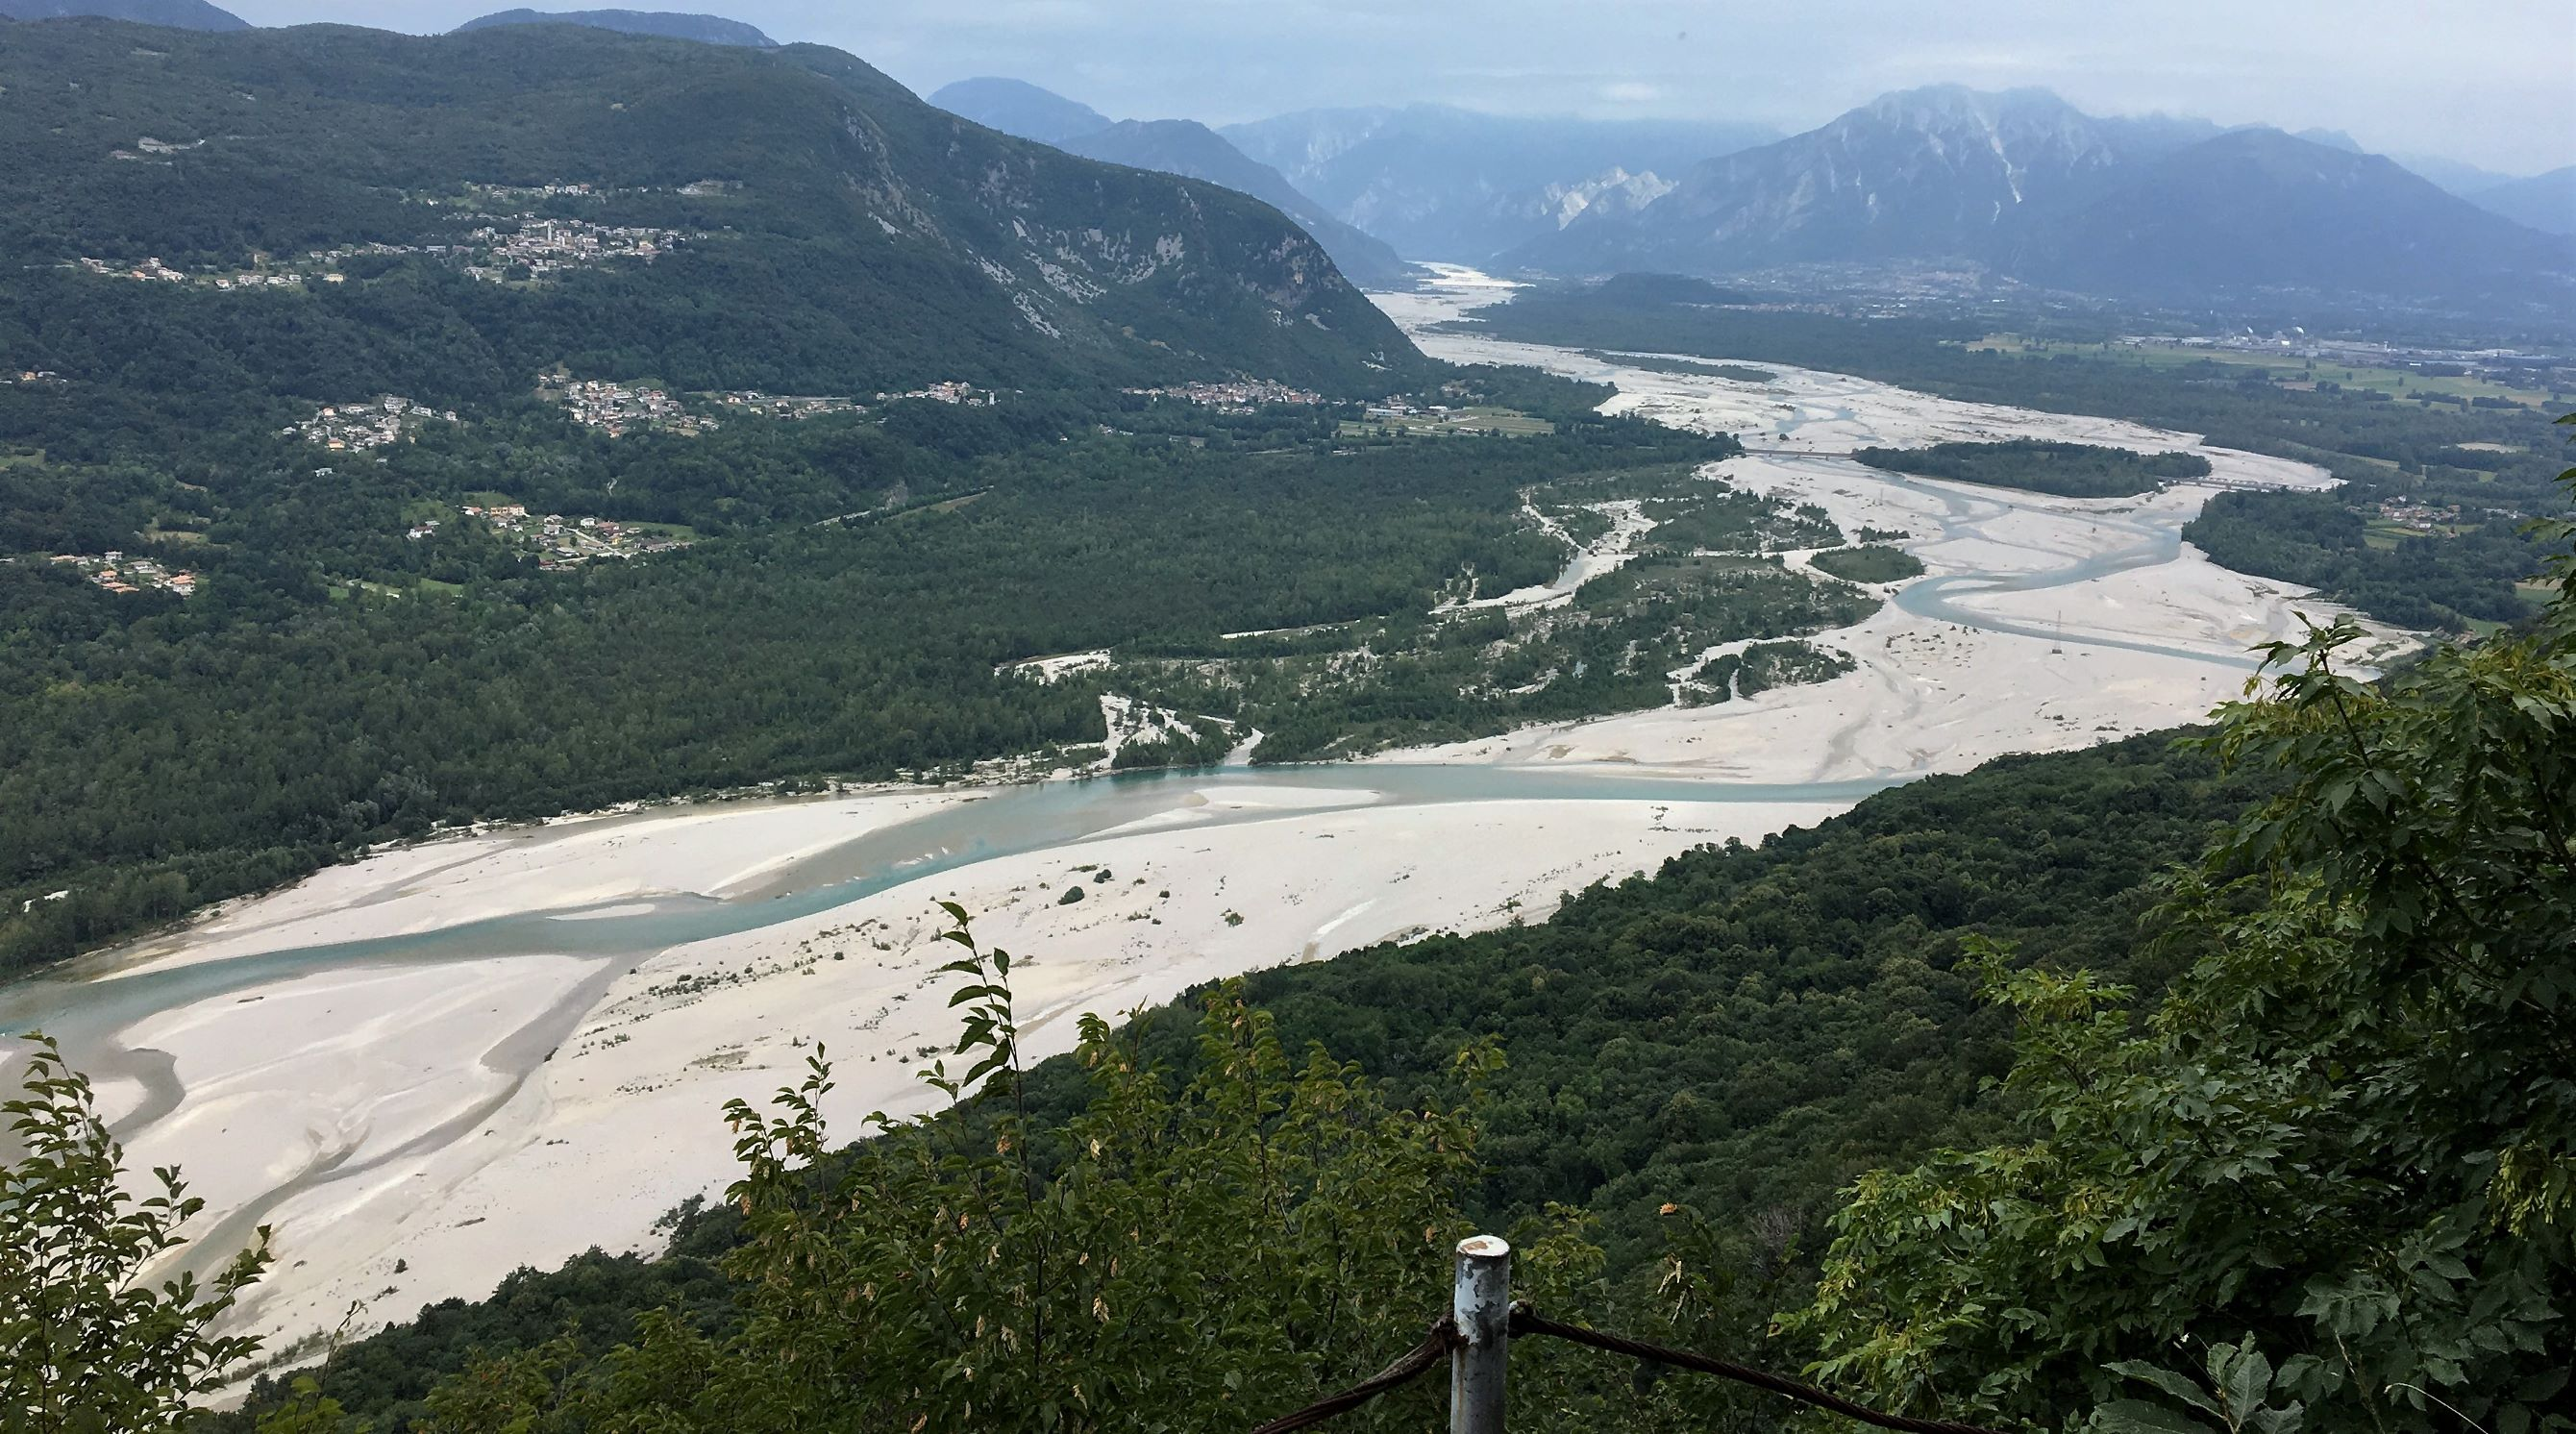
\includegraphics[width=\textwidth]{files/foto_flagogna.jpg}
	\caption[foto di un tratto del Tagliamento ripreso dal monte di Ragogna]{foto di un tratto del Tagliamento ripreso dal monte di Ragogna~(UD); l'acqua scorre da destra verso sinistra.
	}
	\label{fig:foto-ragogna}
\end{figure}



Questa prima figura mostra un fiume che scorre, libero, su un letto di ghiaia che forse pare essere decisamente più largo di quanto gli basterebbe. 
Dove sono gli argini? Il fiume può spostarsi? 
%
In mezzo alla figura si vedono numerose isole divise dal resto della vegetazione da canali abbandonati in ghiaia e sabbia. 
Come si formano? Rimangono inalterate al passare degli anni? 
%
Poco più in basso, dall'altra parte del canale, si intravedono degli arbusti proprio sulla ghiaia. 
Cresceranno fino a formare un'isola tanto vegetata quanto le vicine sue sorelle più a monte? O saranno spazzati via durante la prossima piena?

\medskip
Queste e altre cose si possono leggere da questa foto, così come da quella successiva. Tutte le domande hanno un carattere dinamico più o meno evidente: la loro risposta non la si può ottenere osservando una foto, che è statica, ma una sequenza di istanti successivi quale può essere un filmato.
Come racconta un professore, occorre sincronizzare i nostri orologi con quello del fiume; non solo, bisogna anche che indossiamo gli occhiali giusti per guardare i fenomeni alla scala in cui si possono vedere. Chi mai trarrebbe conclusioni effettive sulla vita di un albero se guardasse solo la sua foglia per pochi secondi, o se lo confrontasse su due immagini satellitari acquisite a distanza di diversi decenni?

\begin{figure}
	\centering
	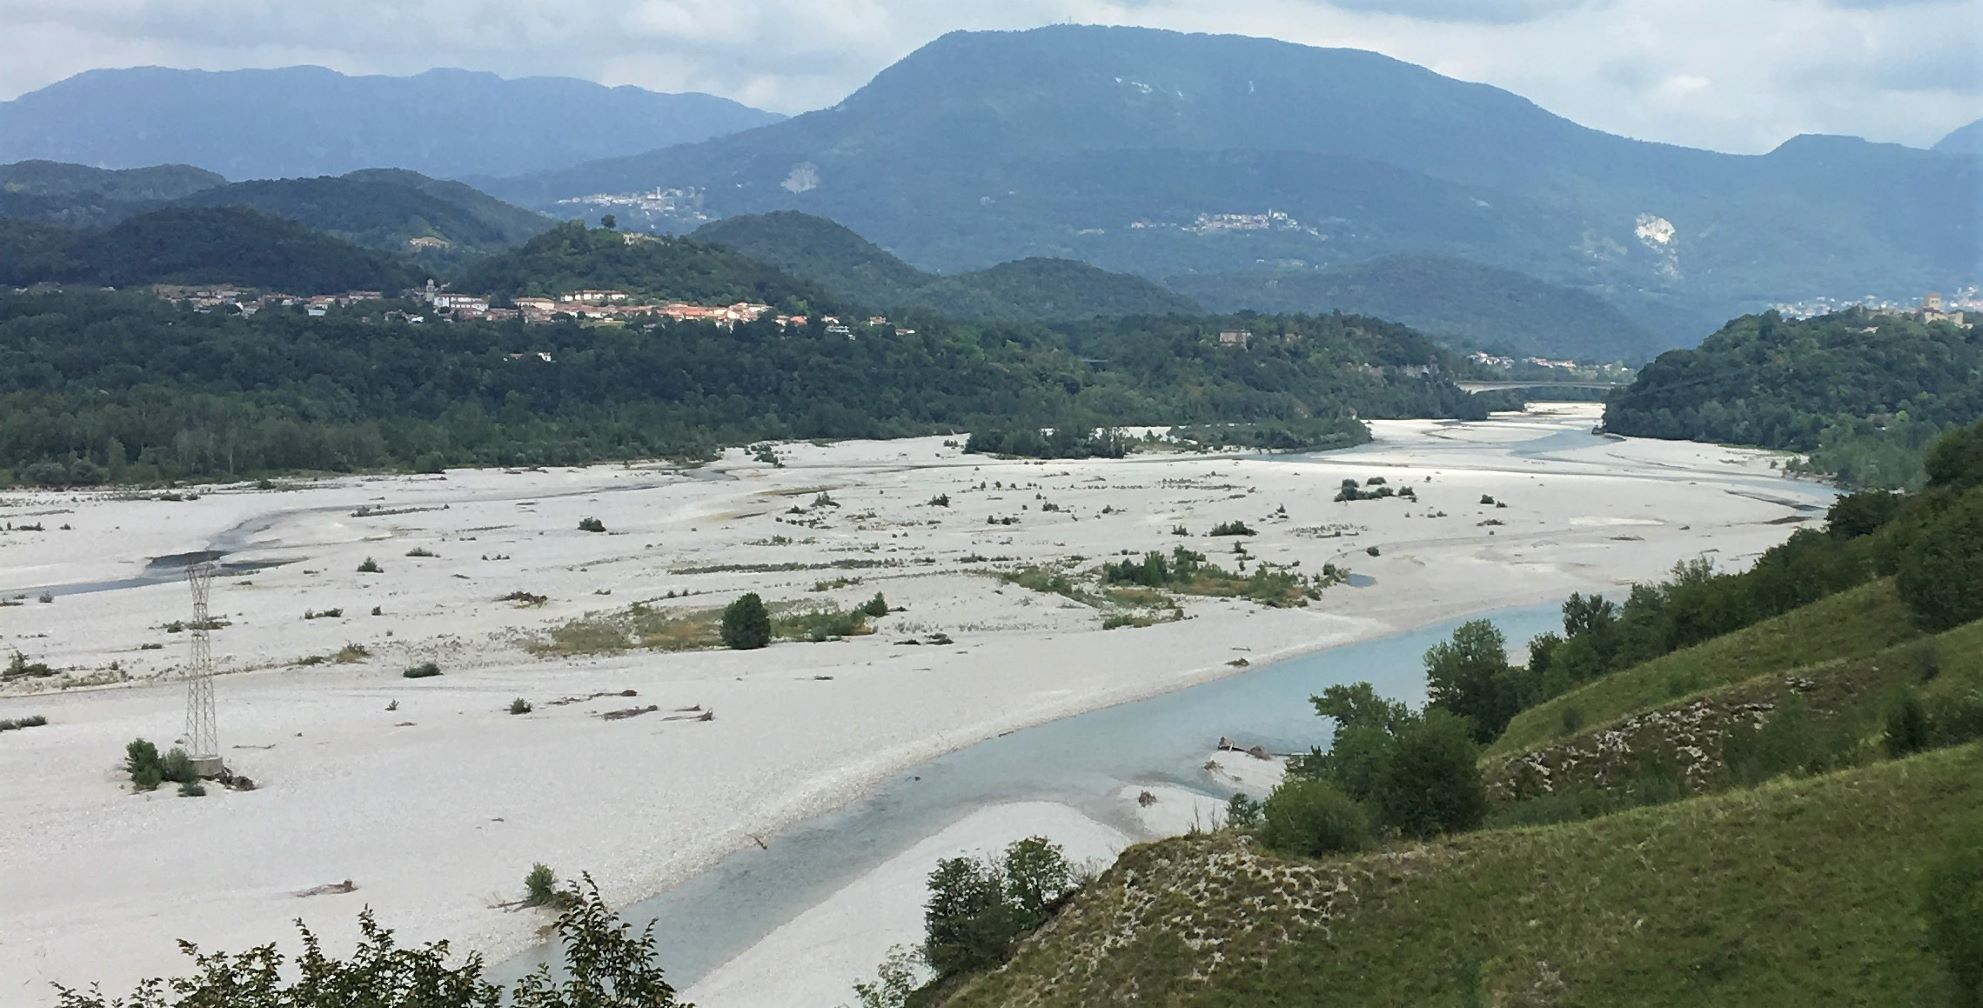
\includegraphics[width=\textwidth]{files/foto_terrazzo_valle_pinzano.jpg}
	\caption[foto di un tratto del Tagliamento ripreso dal terrazzo presso Aonedis~(UD)]{foto di un tratto del Tagliamento ripreso dal terrazzo presso Aonedis~(UD); l'acqua scorre da destra verso sinistra. 
	}
	\label{fig:foto-pinzano}
\end{figure}


Tra tutti i fiumi che ci sono nel nostro bel Paese, pochi di loro sono rimasti in condizioni “naturali”; l'alterazione ha apportato modifiche o ridotto l'entità dei processi che avevano luogo prima dell'intervento dell'uomo. 
Ad esempio, la costruzione di una diga a monte di un fiume può aver indotto nel corso degli anni un restringimento del suo alveo e ad un cambiamento della sua morfologia.
Ma in questo caso siamo fortunati: il Tagliamento può essere considerato un fiume alpino allo stato praticamente naturale.

Le domande che ho posto all'inizio nascono dalla curiosità che si può avere quando, dopo mesi di studio dei fenomeni che naturalmente avvengono nei fiumi, si incontra un fiume dove questi fenomeni possono accadere per davvero. Le domande trovano una risposta reale, comprovata da ciò che si vede quando si cammina sulla ghiaia, in mezzo alle isole, nei canali, e quando ci si tuffa nelle loro confluenze.

\medskip
La \cref{fig:confronto-imm-prefaz} mostra diversi processi che avvengono in questo fiume; questi, inutile ripeterlo, diventano apprezzabili solo dopo aver indossato gli occhiali e l'orologio giusti, cioè osservando da un'altezza di poche centinaia di metri da terra e confrontando immagini distanti pochi mesi. Ecco un'anteprima:
\begin{itemize}
	\item si vede subito che i canali migrano e si spostano durante gli anni; 
		difatti durante le piene più importanti tutto l'alveo si riempie di acqua e il fondo viene rimodellato;
	\item lo spostamento dei canali porta questi ad erodere lateralmente le isole, come si vede per l'isola in alto a sinistra in alveo; 
		il fiume quindi potrà trasportare non solo il materiale presente sul fondo, ma anche quello che erode dalle isole, sia ghiaia e sabbia che alberi;
	\item le isole possono espandersi da piccoli nuclei fino a unirsi, diventare più fitte e più resistenti all'erosione da parte dell'acqua, come si vede per la grande isola al centro della \cref{fig:confronto-imm-prefaz};
	\item l'erosione non risparmia le sponde, come si vede per la sponda a sinistra (in destra idrografica se si osserva il verso della corrente) la quale arretra di più di \SI{100}{\m} a causa delle piene che si susseguono nei tre anni di osservazione;
	\item l'erosione di isole e sponda produce moltissimo materiale legnoso (alberi sradicati) il quale si deposita poco più a valle della zona di erosione, come testimoniano i numerosi puntini scuri presenti sull'alveo asciutto; 
		se le condizioni sono adatte e se le piante sono in grado, è possibile che dai tronchi depositati crescano nuovi rami e radici; 
		questi tronchi diventano i nuclei di formazione di future isole;
	\item lo spostamento dei canali è limitato dalla presenza delle isole, che si configurano come ostacolo per la corrente anche durante le piene;
		difatti è difficile che il canale si possa spostare dove c'è l'isola in alto a destra, a meno che non riesca ad eroderla.
\end{itemize}

\begin{figure}
	\centering
	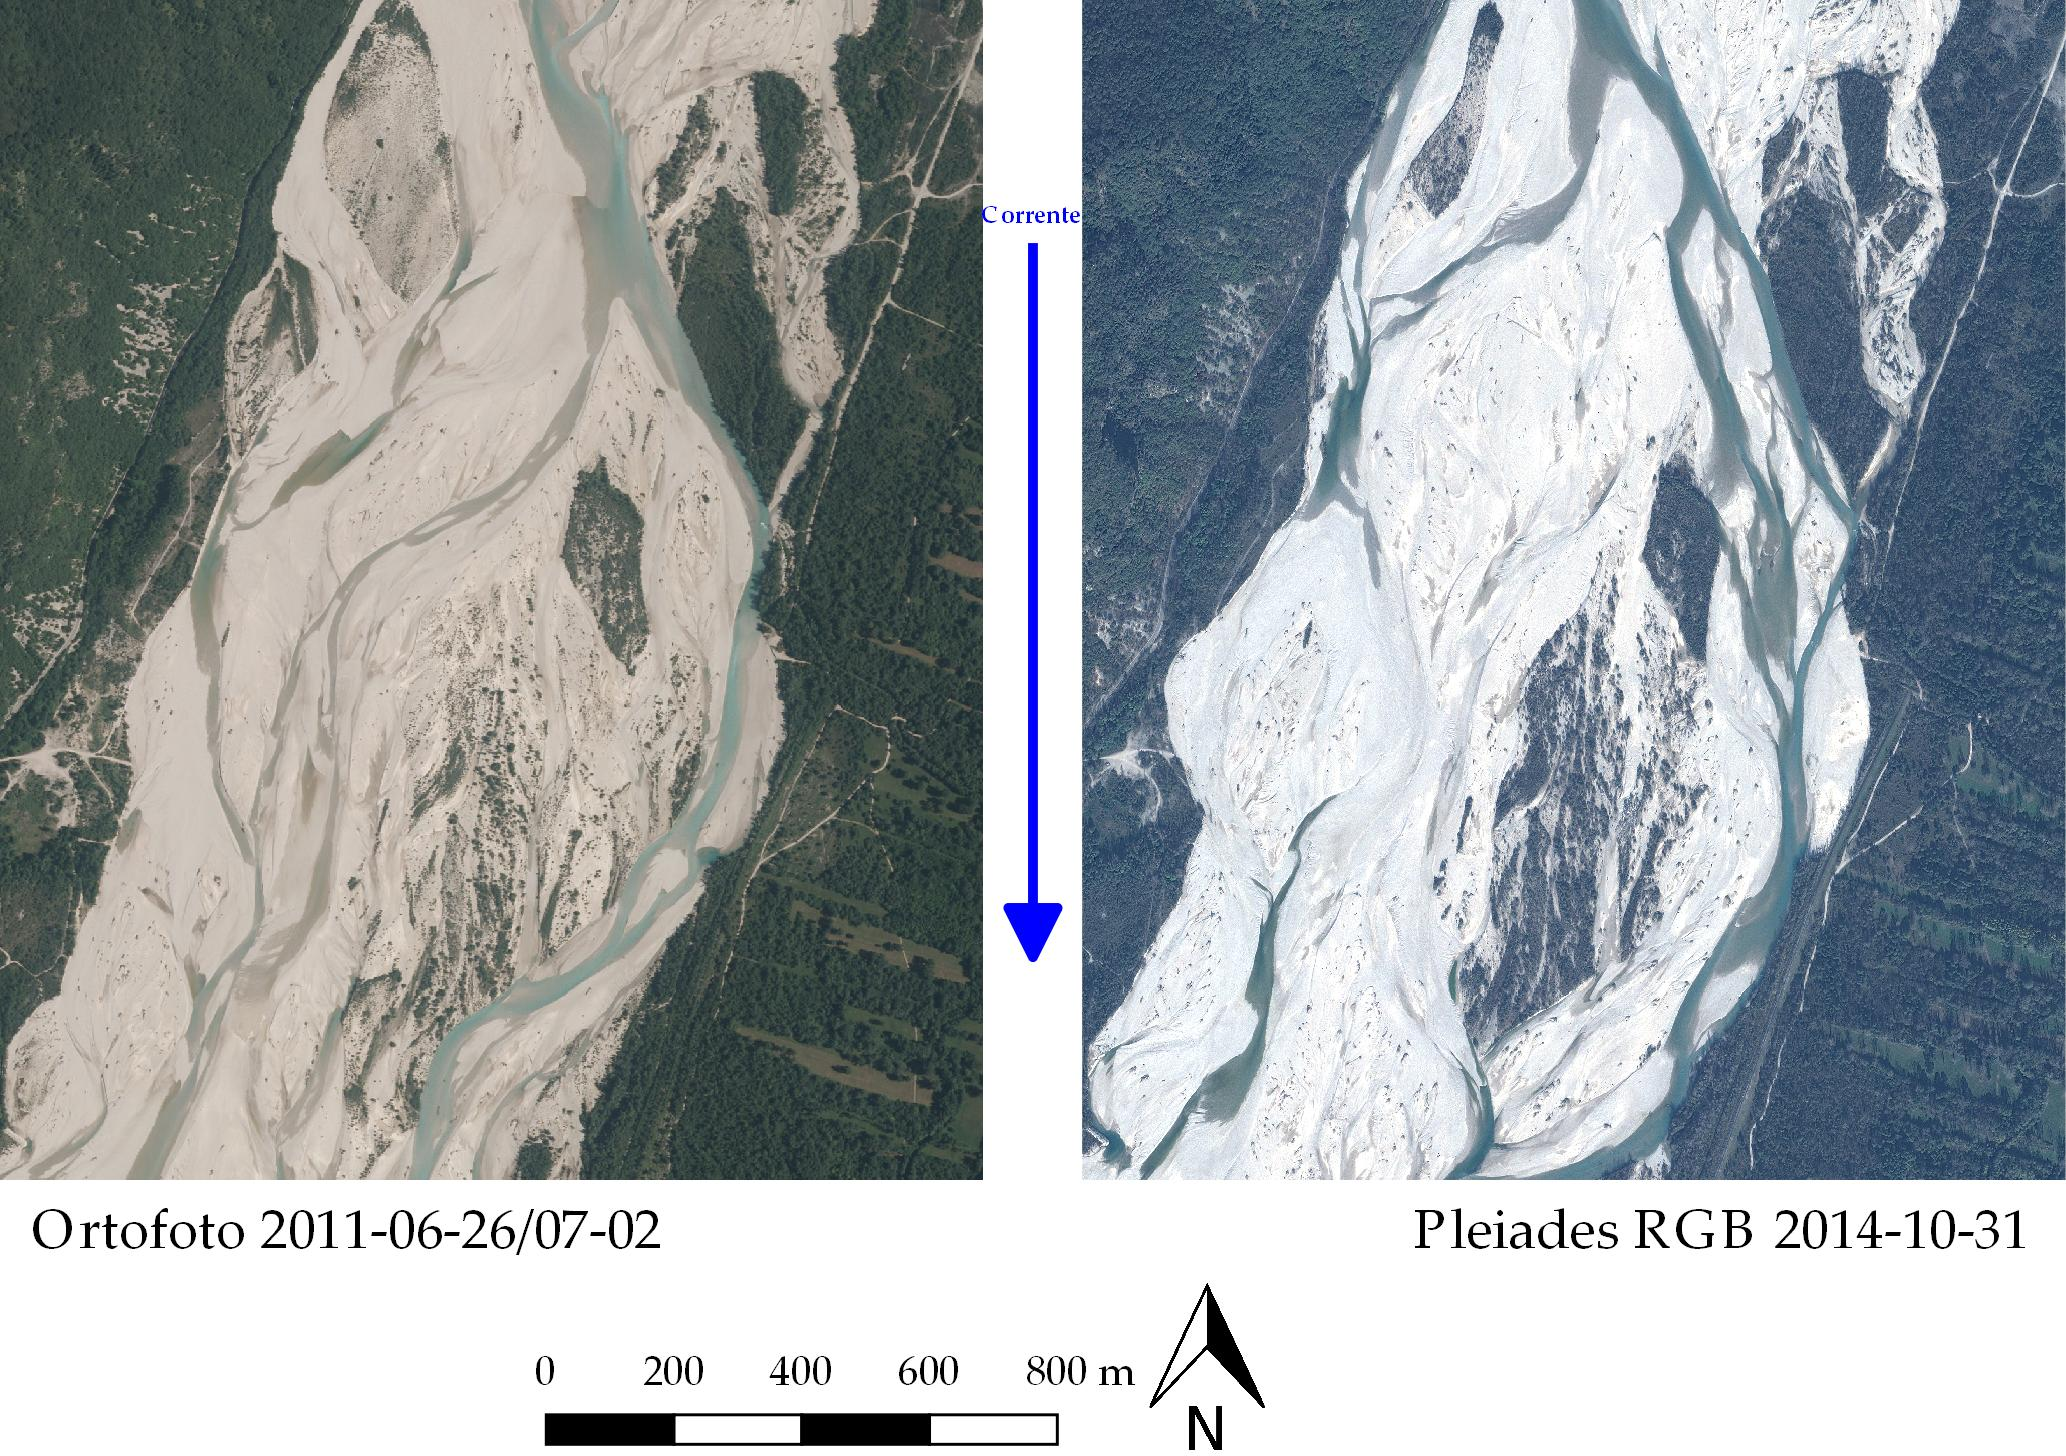
\includegraphics[width=\textwidth]{files/confronto_immagini_erosione_isole.jpeg}
	\caption[immagini di un tratto posto circa \SI{2}{\kilo\m} a monte del ponte di Cornino]{immagini di un tratto posto circa \SI{2}{\kilo\m} a monte del ponte di Cornino~(UD); l'ortofoto proviene dal Portale Cartografico Nazionale del Ministero dell'Ambiente.
	}
	\label{fig:confronto-imm-prefaz}
\end{figure}


Quante cose si possono osservare! In un fiume siffatto sono presenti numerosi altri fenomeni anche a scale diverse.
Ho raccontato quelli che mi interessano particolarmente e che sono oggetto di questa tesi: le dinamiche della vegetazione sulle isole e le dinamiche del legno depositato in alveo.

\medskip
A pensarci bene, non è sorprendente che in un sistema naturale la componente biologica influenzi fortemente quella fisica: i boschi consolidano i pendii e le foreste determinano la forma meandriforme di molti fiumi. Attraverso altri esempi ci si può convincere che le isole vegetate e i tronchi che rigettano in arbusti possano esercitare effetti su un fiume e viceversa. 
\\
E riflettendo ancora non è difficile osservare che queste interazioni solitamente possono indurre effetti positivi sia per l'ambiente che per l'essere umano: per portare qualche esempio, nel caso del Tagliamento si parla di biodiversità data da un mosaico in continuo cambiamento di ambienti diversi, di purificazione dell'acqua, del mantenimento di un microclima particolarmente adatto alla stagionatura del prosciutto di San Daniele (prodotto nell'omonimo paese poco distante) e di un luogo molto adatto per la ricreazione da parte delle persone (\cref{fig:bagnanti}).

Da questi fatti muovo i primi passi verso l'approfondimento dei processi che portano un fiume a modificarsi di continuo assieme all'ambiente in cui si colloca.


\begin{figure}[hb]
	\centering
	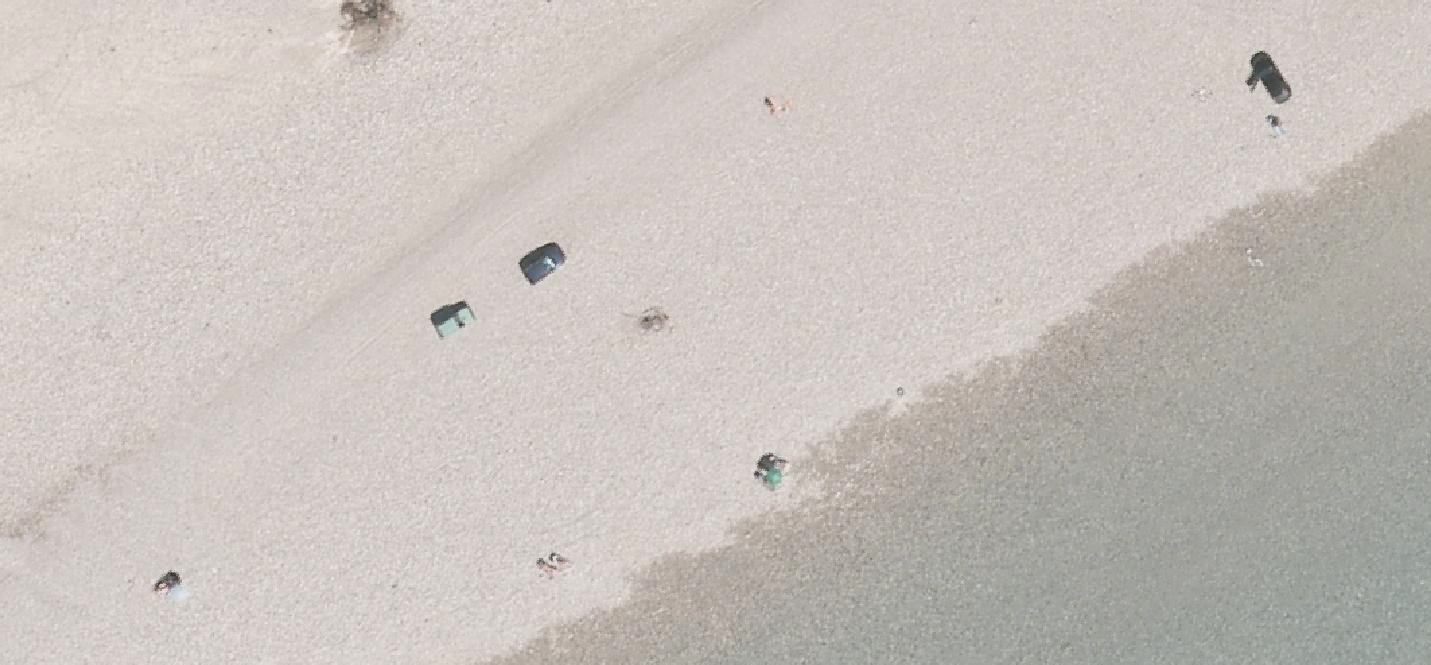
\includegraphics[width=\textwidth]{files/bagnanti.jpeg}
	\caption[bagnanti accanto ad un canale]{bagnanti accanto ad un canale ripresi con una immagine area del~2011, cortesemente fornita da Nicola Surian (Università degli studi di Padova).}
	\label{fig:bagnanti}
\end{figure}



%----------------------------------------------------------



%**********************************************************
%**********************************************************
\mainmatter
\chapter{Introduzione}
\section{L'area di studio: il Tagliamento}
\label{sec:descr-area-studio}
\paragraph{Inquadramento}
Nei fiumi a morfologia intrecciata dove l'impatto antropico non è intenso è possibile trovare isole nell'alveo dove il disturbo indotto dalle piene non è eccessivo;
queste si formano e accrescono nel periodo compreso tra eventi di piena di una certa entità, mentre vengono erose dagli eventi idrologici sufficientemente intensi \squarecites{Poff:1997}{Gurnell:2001-island-formation}.
La presenza delle isole ha un importante ruolo ecologico: la varietà spaziale e temporale di ambienti presenti (pozze d'acqua, sorgenti e canali separati da aridi sedimenti, zone con vegetazione bassa e rada alternate con isole fitte e mature che si modificano tra e in seguito alle piene) crea un mosaico in continuo cambiamento che sostiene una forte biodiversità \squarecites{Arscott:2002-habitat-dynamics}.
Inoltre, durante piene di piccola entità le piante influenzano l'accrescimento delle forme fluviali attraverso la ritenzione di sedimenti e materiale legnoso sia morto che vivo, inducendo così la successiva colonizzazione da parte di altre piante e la rimodellazione dei canali \squarecite{Gurnell:2006-omega}.


Il Fiume Tagliamento, situato nel Nord-Est italiano, è uno dei pochi fiumi alpini allo stato quasi naturale che presenta queste caratteristiche. 
Sono stati effettuati interventi di ingegneria fluviale, come arginature, derivazioni, pennelli, estrazione di ghiaia, sia in tratti posti a monte che in altri posti a valle; la loro entità è comunque tanto limitata da poter parlare di “contesto non gestito”.
\\
Difatti il Tagliamento presenta un regime idrologico non alterato, con piene frequenti ed imprevedibili dovute all'alta piovosità nel bacino \squarecites{Mosetti:1983}{Bertoldi:2009-2m} e alla limitata presenza di bacini di regolazione (solo il \SI{3}{\percent} dell'area drenante del bacino è intercettata da dighe \squarecite{Sitzia:2016-d50});
è stato suggerito che è possibile formulare previsioni accurate di un evento di piena solamente nelle 5 ore precedenti \squarecite{Arscott:2002-habitat-dynamics}. 
Inoltre, le sponde e l'alveo sono colonizzate da ampie porzioni di vegetazione riparia lungo quasi tutto il suo corso. 
Questi fatti indicano che le attività umane sul Tagliamento non sono tali da aver alterato o da alterare il regime del fiume.

Il bacino idrografico del Tagliamento, ampio circa~\SI{2900}{\kilo\m\tothe{2}}, si estende tra le province di Belluno, Udine, Pordenone e Venezia.
Il suo corso di circa~\SI{170}{\kilo\m} presenta morfologia intrecciata (\emph{braided}) con canali multipli separati da barre e isole.
Nelle parti montane è confinato dai versanti; 
nella parte planiziale è libero, con tratti larghi diverse centinaia di metri, se non più di \SI{1}{\kilo\m};
a qualche decina di chilometri dalla foce il fiume si restringe assumendo prima una forma transizionale monocursale con larghezza sui \SIrange[range-phrase={-}]{300}{200}{\m} nei pressi di Madrisio~(UD);
infine diventa meandriforme a Latisana~(UD) (larghezza intorno ai \SI{100}{\m}) fino alla foce, situata tra Bibione~(VE) e Lignano~(UD).
\\
Insieme alla variazione della morfologia del fiume si assiste ad un cambiamento nella granulometria: mentre la ghiaia predomina nella parte intrecciata ($d_{50} = \SI{4}{\centi\m}$ \squarecites{Bertoldi:2010-d50}{Sitzia:2016-d50}), a partire dal tratto meandriforme si trova solo sabbia sul fondo.
Questo mutamento di materiale trasportato riflette la riduzione della pendenza che si osserva dal tratto transizionale monocursale e che giustifica il passaggio da fiume “in ghiaia” a fiume “in sabbia”.
\\
Le precipitazioni sono mediamente di circa \SI{2000}{\mm} all'anno con forti variazioni locali; i minimi di precipitazione si registrano durante l'inverno, mentre i massimi in primavera e in autunno.
Si assiste anche ad eventi di breve durata e particolarmente intensi.
Il regime fluviale che ne risulta è di tipo \emph{flashy} pluvio-nivale con piene brevi ed intense così come piene di diversi giorni di durata.

Il tratto studiato è quello intrecciato multicanale compreso tra Tolmezzo~(UD) e Madrisio~(UD) (\cref{fig:overview,fig:overview-sat}). 
%
\begin{figure}
	\centering
	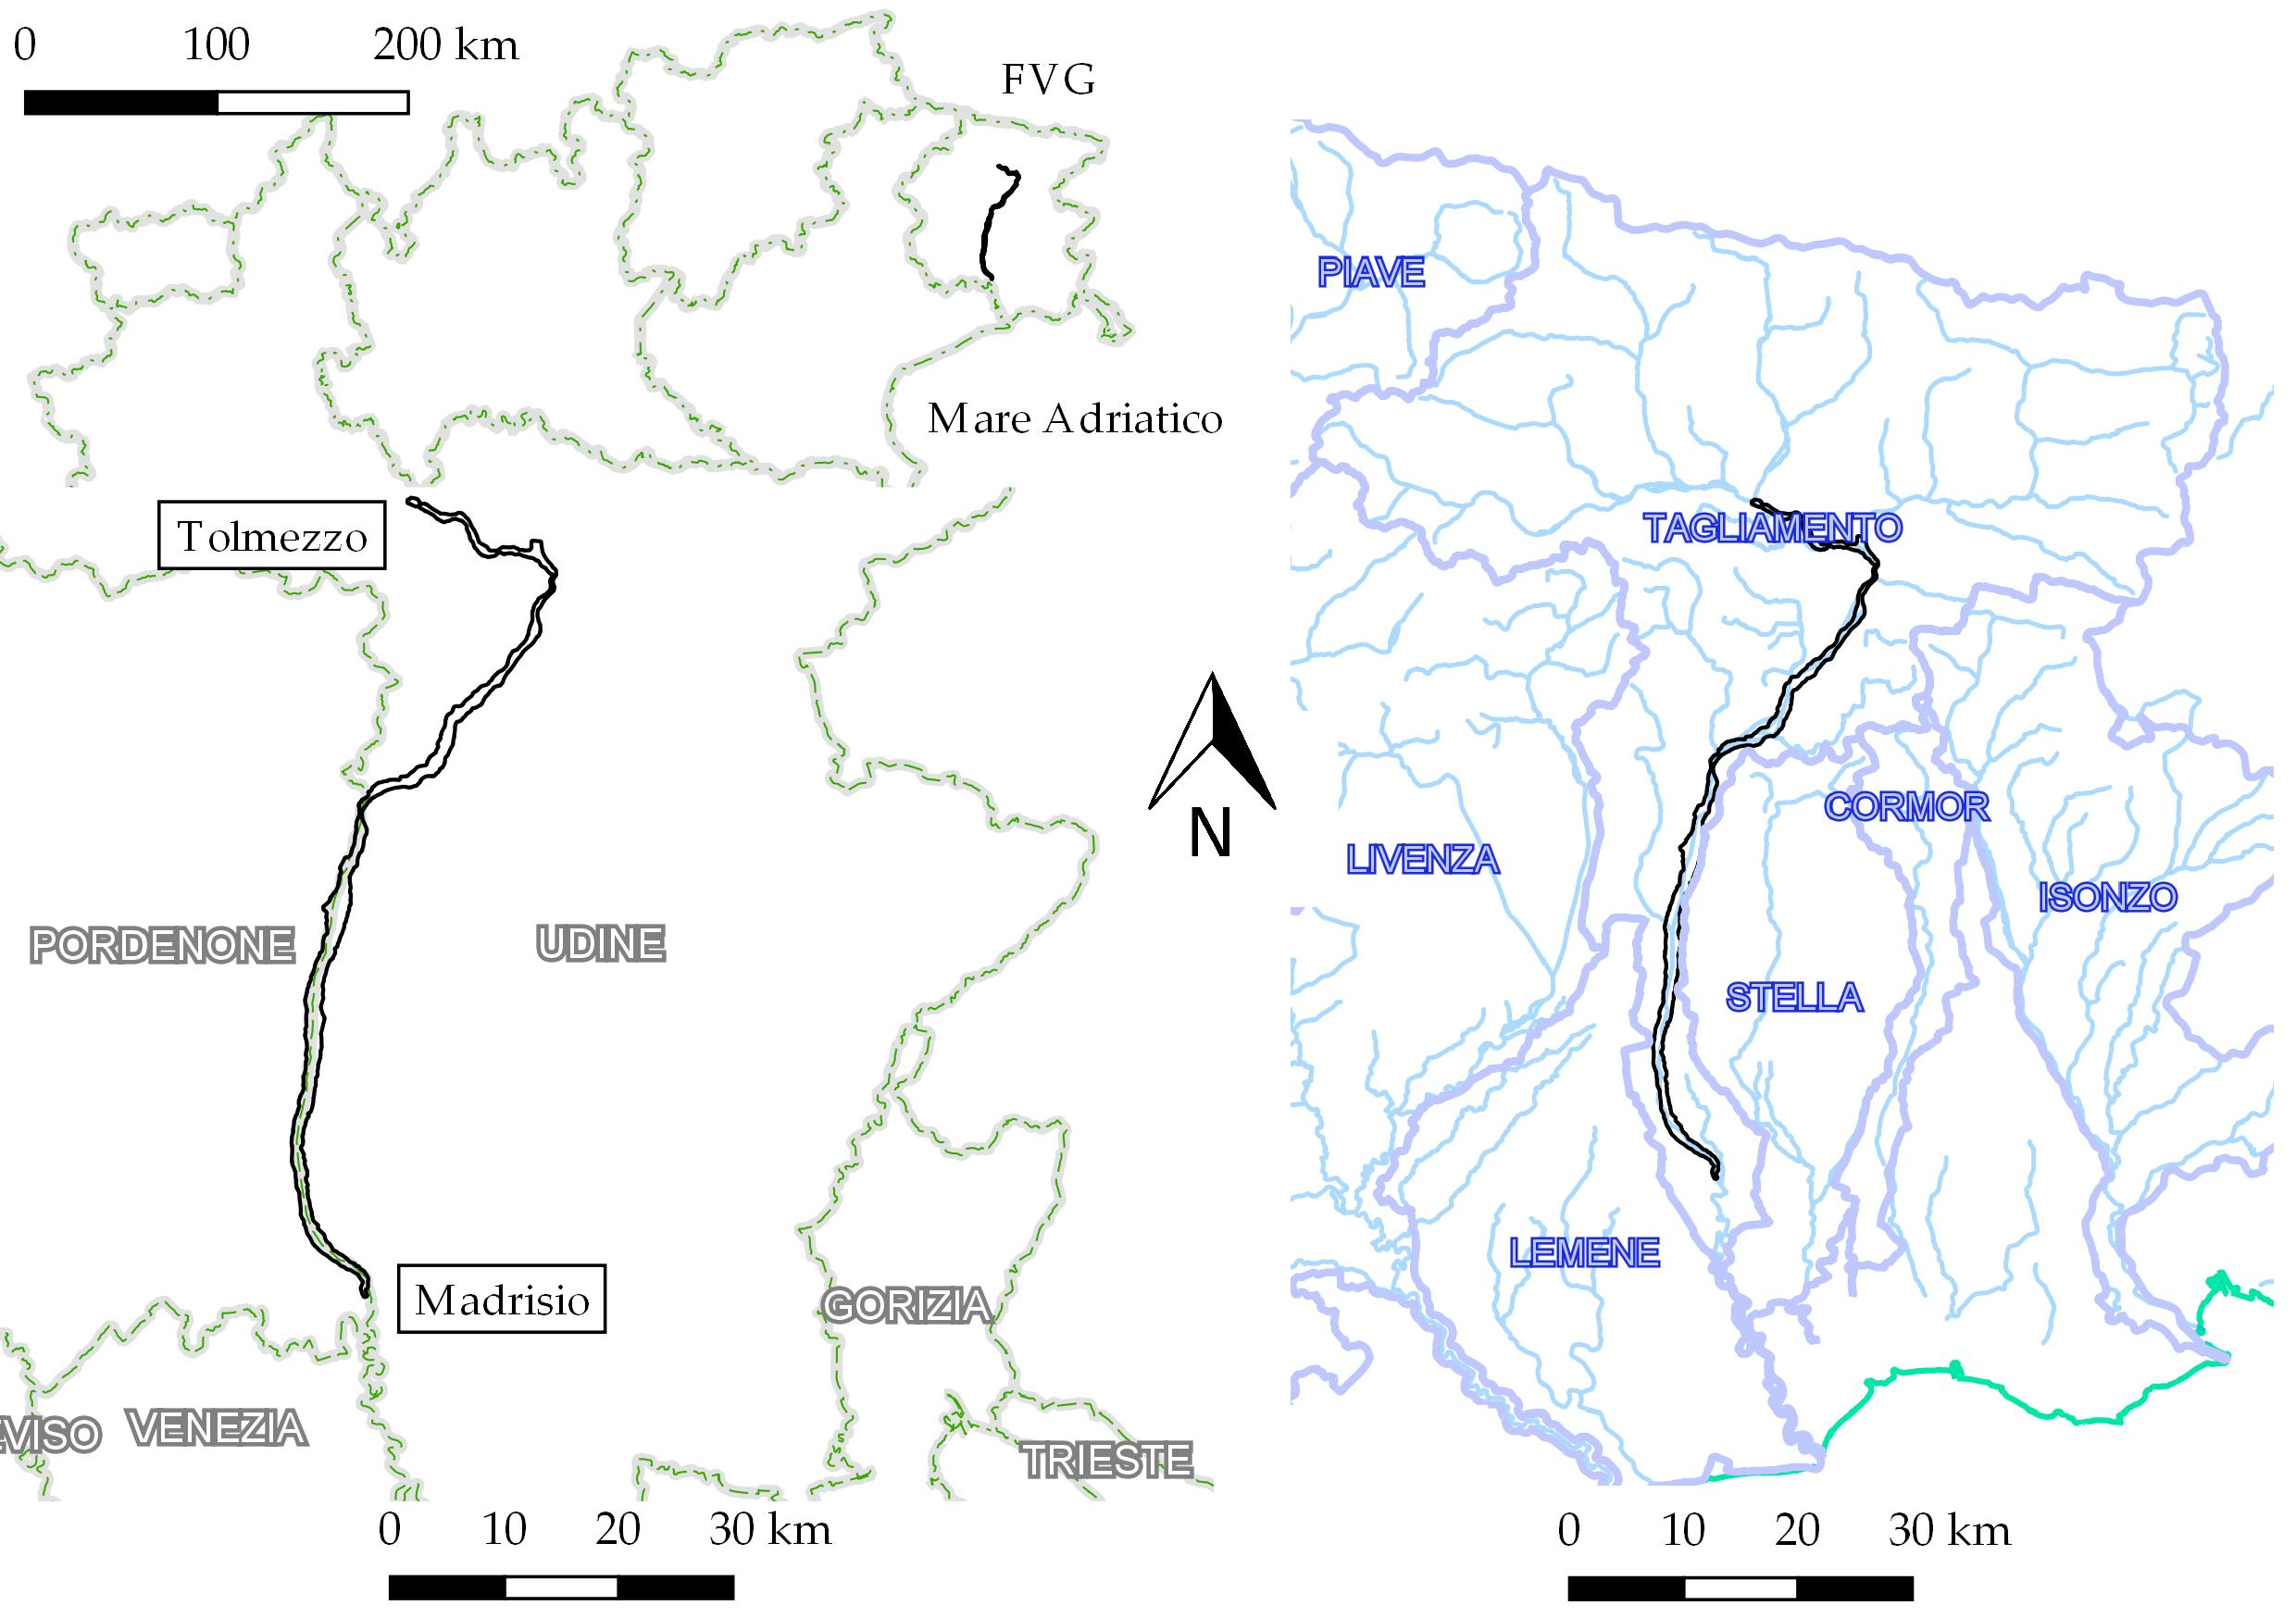
\includegraphics[width=\textwidth]{files/overview.jpeg}
	\caption[inquadramento dell'area di studio]
		{inquadramento dell'area di studio (poligono nero); a sinistra è mostrata l'Italia settentrionale (in alto) e un ingrandimento delle province e degli estremi dell'area di studio (in basso); a destra si vede il bacino idrografico del Tagliamento e di altri fiumi nelle vicinanze (in blu), il reticolo idrografico (in azzurro) e la linea di costa (in verde acqua). I tematismi provengono dal Portale Cartografico Nazionale del Ministero dell'Ambiente.}
	\label{fig:overview}
\end{figure}
%
\begin{figure}
	\centering
	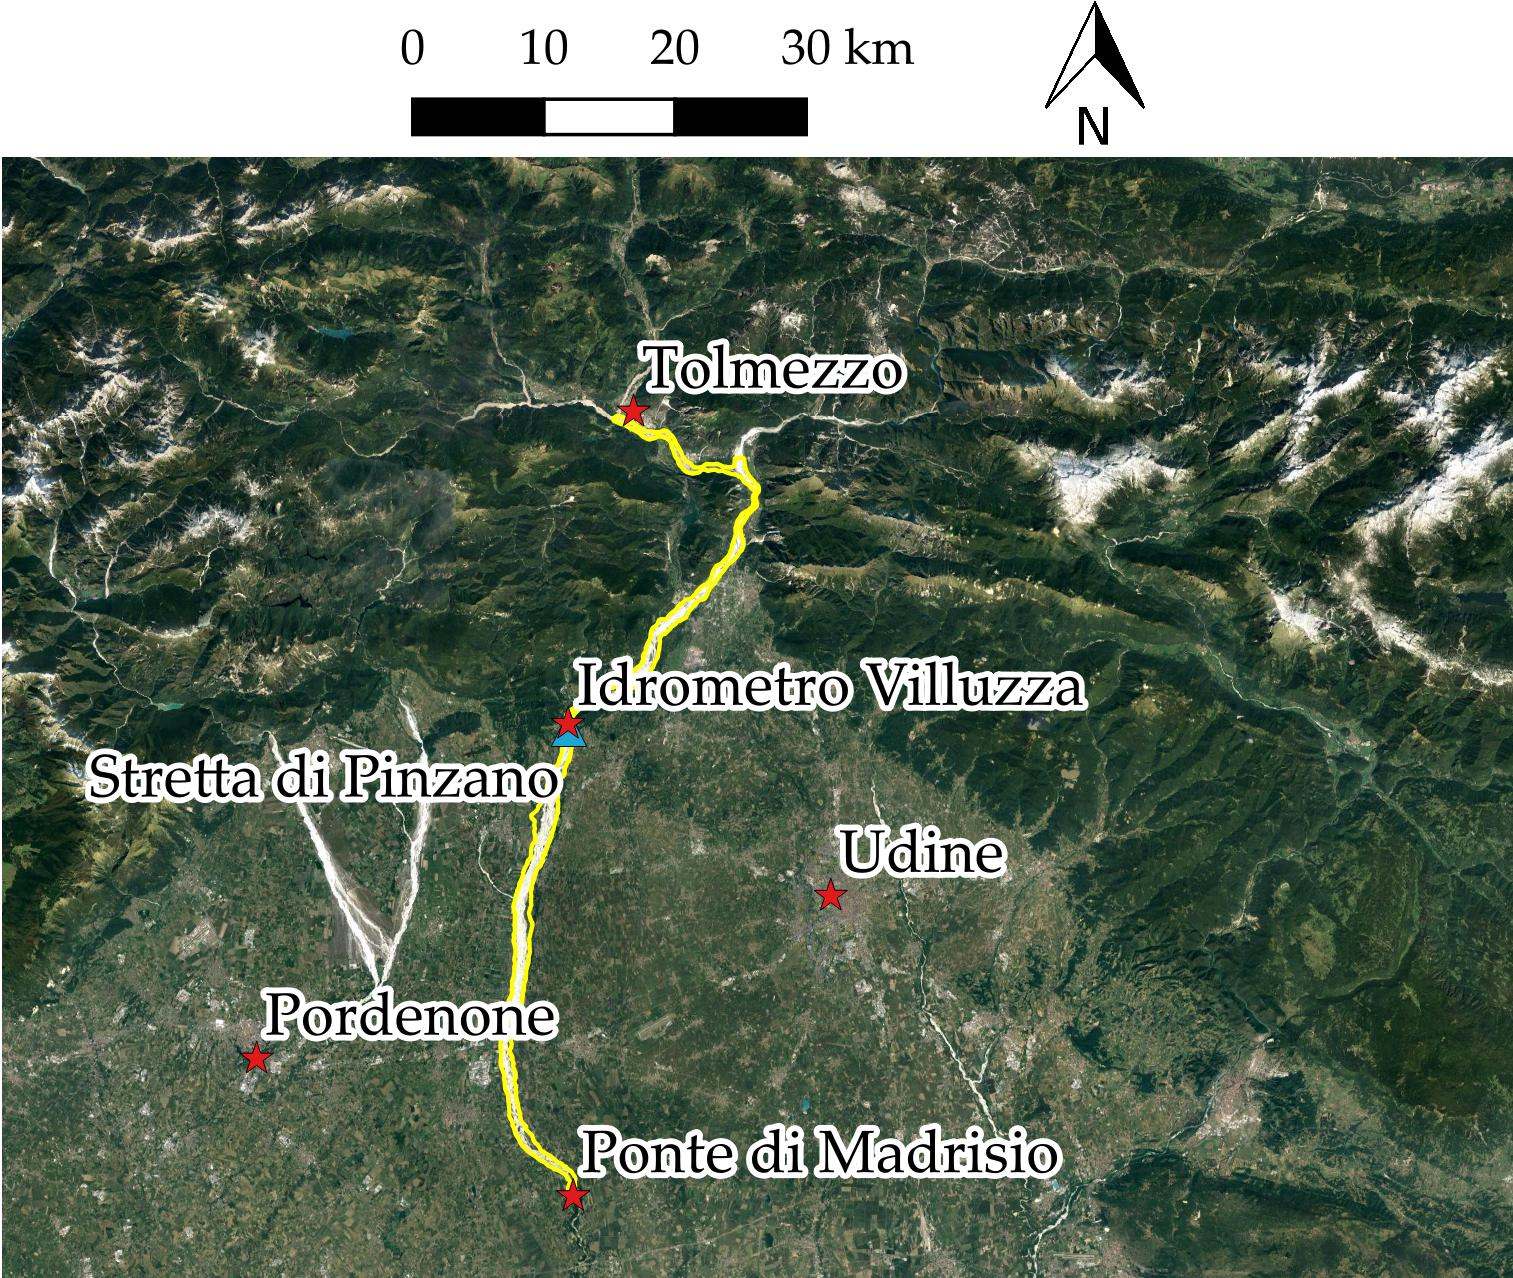
\includegraphics[width=\textwidth]{files/overview_tratto_sat.jpeg}
	\caption[inquadramento dell'area di studio]{inquadramento dell'area di studio (contornata in giallo) assieme ad alcune zone di interesse.
	\\
	Map data: Google, Digital Globe.}
	\label{fig:overview-sat}
\end{figure}
%
\\
L'area di studio è stata suddivisa manualmente in 23~tratti al fine di avere un maggior dettaglio spaziale delle dinamiche di vegetazione (\cref{fig:23-tratti}). 
Questi tratti sono stati selezionati in modo da possedere caratteristiche omogenee per portata e crescita della vegetazione; 
pertanto confluenze di immissari, bruschi restringimenti o allargamenti, inizio di pronunciato \emph{upwelling} o \emph{downwelling} ed evidenti cambiamenti di morfologia fluviale sono stati gli elementi per individuare i 23~tratti.
%
\begin{figure}
	\centering
	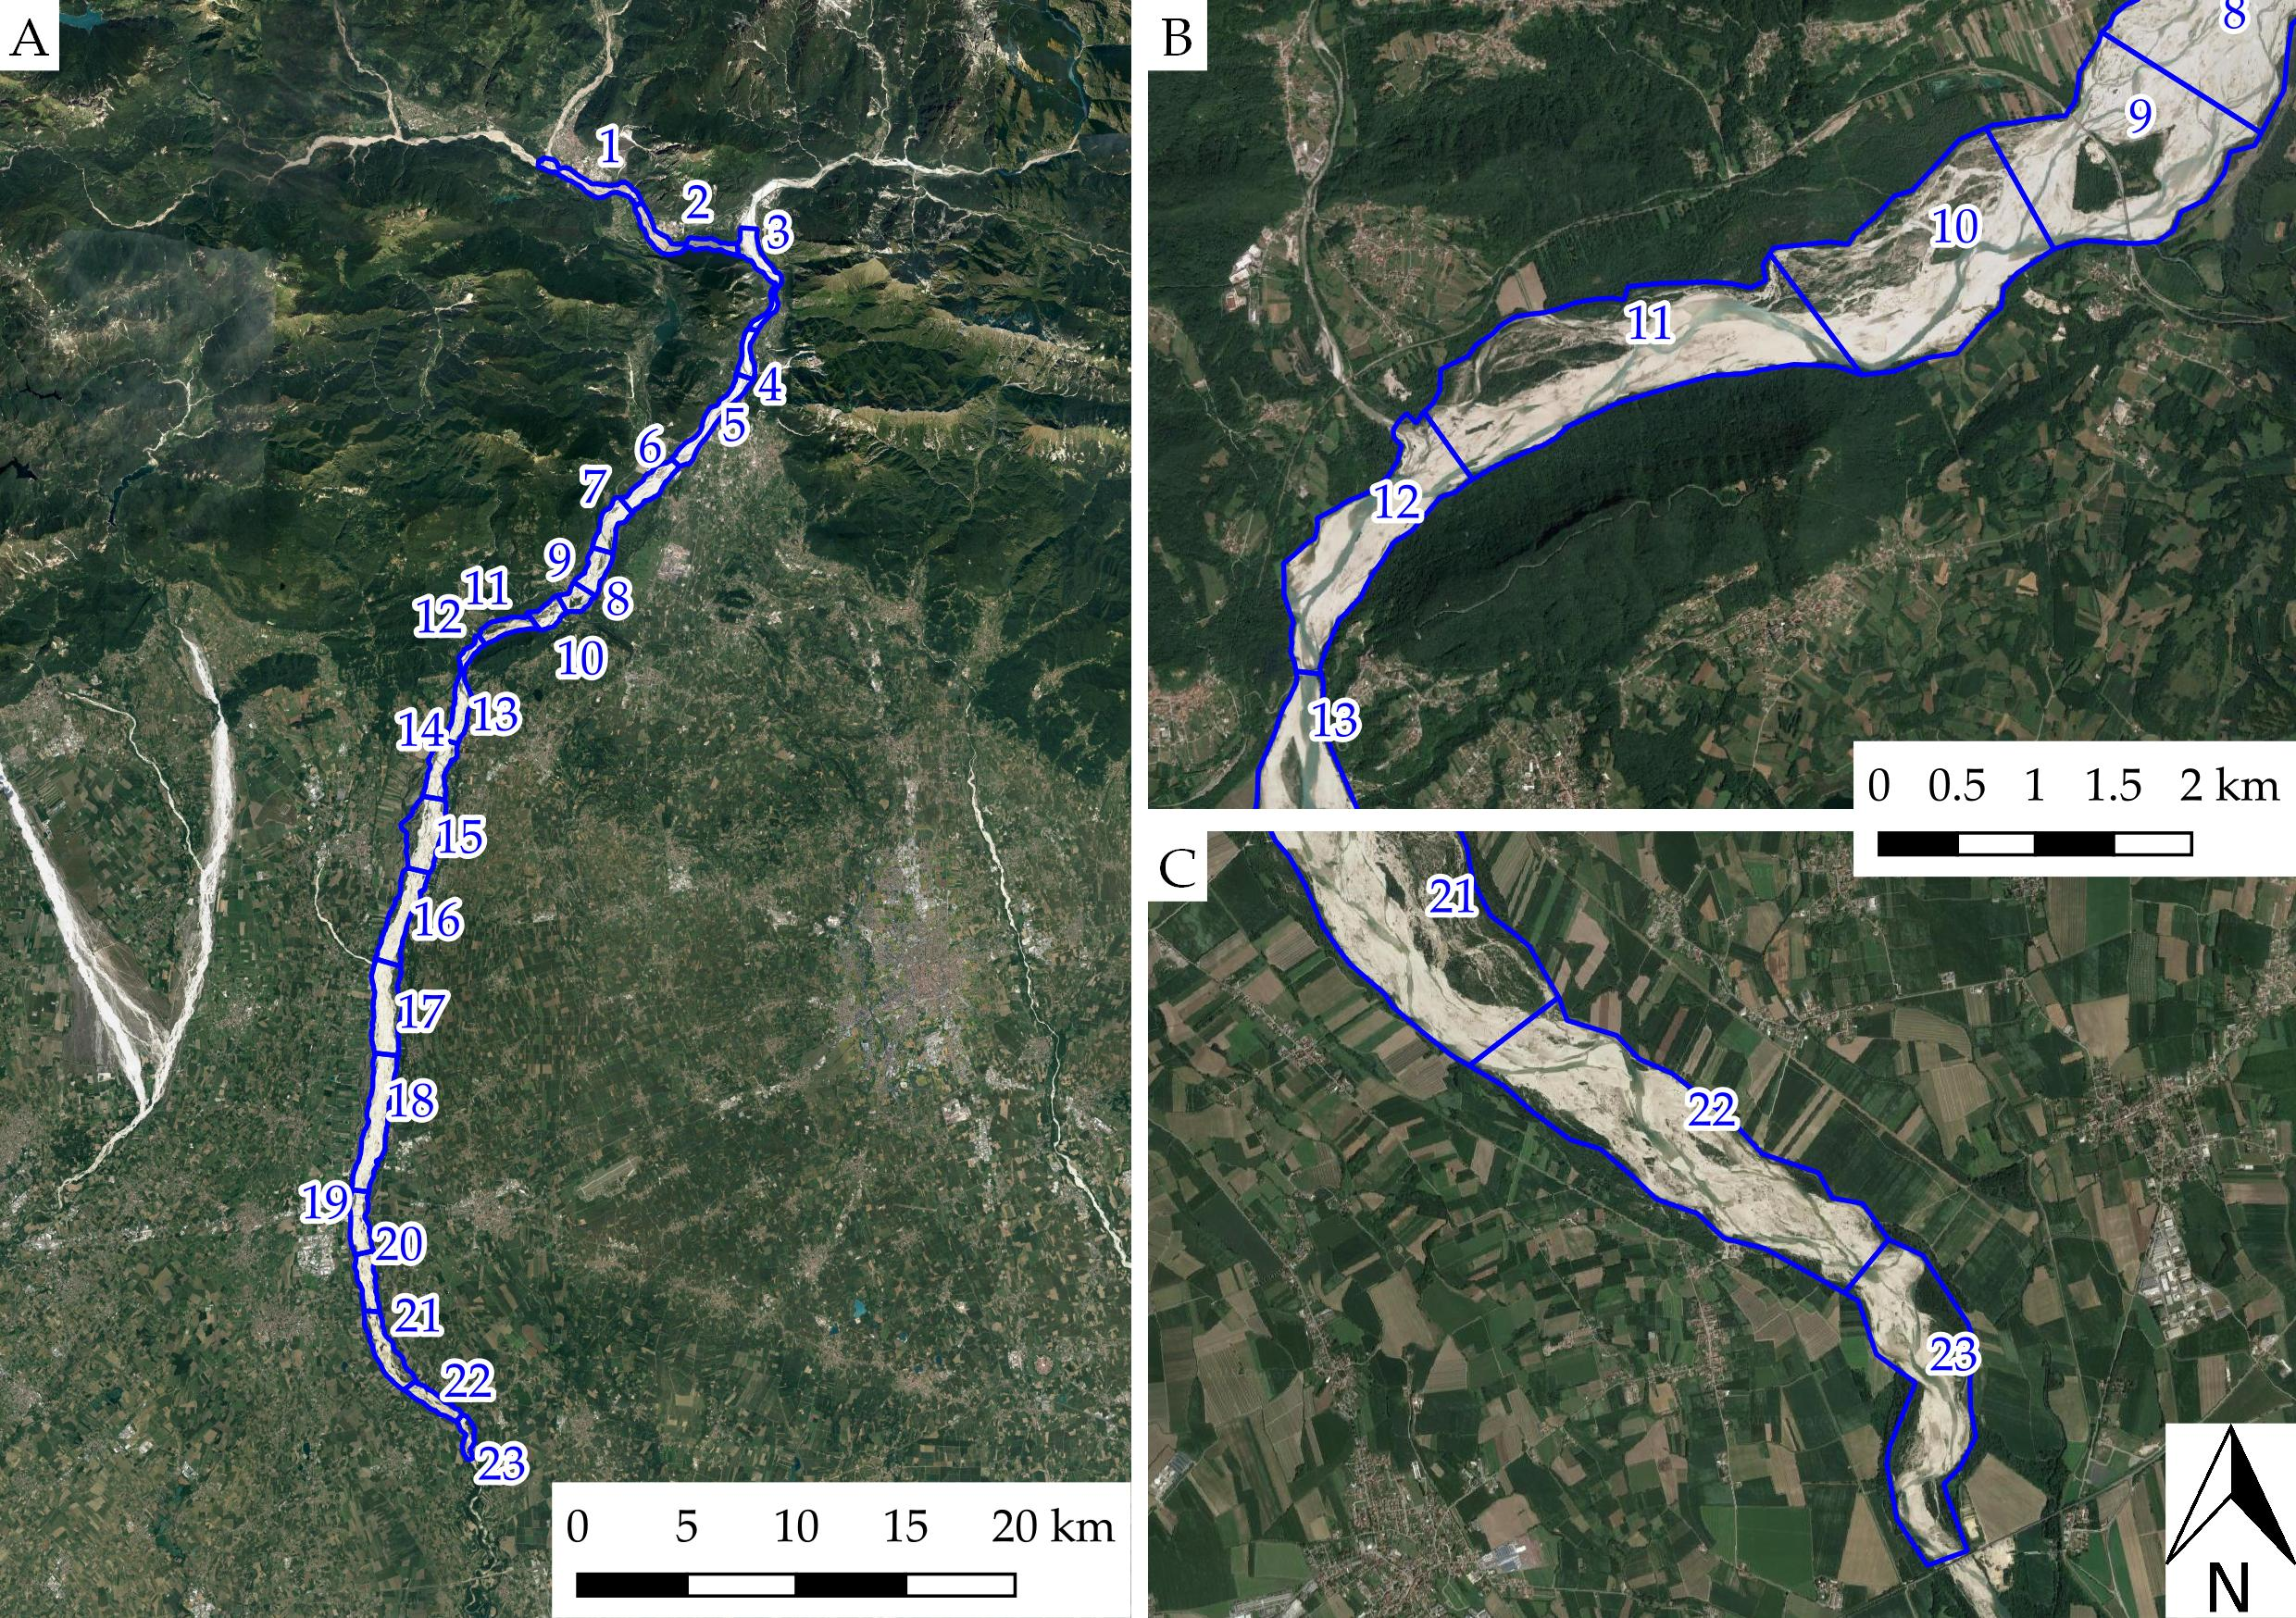
\includegraphics[width=\textwidth]{files/tutti_23_tratti.jpeg}
	\caption[immagine dei 23 tratti in cui è suddivisa l'area di studio]{immagine dei 23 tratti in cui è suddivisa l'area di studio (figura~A); la sezione di monte del tratto~1 corrisponde a Tolmezzo, la sezione di valle del tratto~23 corrisponde al ponte di Madrisio. A destra sono mostrati ingrandimenti dei tratti presso l'isola di Cornino (tratto~9) e la stretta di Pinzano (tra il tratto~12 e il~13) (figura~B) e nei tratti dove la morfologia diventa transizionale poco a monte di Madrisio (tratti~22 e~23) (figura~C).
	\\
	Map data: Google, Digital Globe.}
	\label{fig:23-tratti}
\end{figure}


\paragraph{Connessione con la falda}
Nel tratto di studio nei pressi del paese di Pinzano al Tagliamento~(PN) è presente una stretta causata dall'affioramento di strati rocciosi che riduce la larghezza da diverse centinaia di metri a circa \SI{130}{\m}.
Questo restringimento, congiuntamente all'innalzamento dello strato di roccia che si trova sotto il letto del fiume, induce variazioni longitudinali nel livello di falda nel materasso alluvionale.
L'acqua filtrante da monte risale in alveo sotto forma di sorgenti diffuse: si assiste al fenomeno dell'\emph{upwelling}.
A valle della stretta, dove l'alveo non è più confinato e il letto roccioso sprofonda nel sottosuolo, l'acqua torna ad infiltrarsi nel materasso ghiaioso (\emph{downwelling}) tanto da portare il fiume in condizioni di secca in certi tratti quando non ci sono piene.
\\
L'\emph{upwelling} e il \emph{downwelling} sono fenomeni rilevanti durante i periodi di magra: certi tratti a valle della stretta di Pinzano possono essere in condizioni di secca, privi completamente di acqua, la quale scorre tutta nel sottosuolo e riemerge presso la “Linea delle risorgive” \squarecite{Mosetti:1983}, quando la morfologia fluviale diventa transizionale pochi chilometri a monte del ponte di Madrisio.
\\
Durante le piene questi fenomeni sono invece irrilevanti: l'acqua che emerge o che si infiltra contribuisce minimamente alla portata fluente.
\\
Il moto di infiltrazione contribuisce al mantenimento di una forte biodiversità caratteristica dell'ambiente fluviale, oltre a permettere una costante purificazione dell'acqua fluente in periodi di magra.

\paragraph{Affluenti}
Nel tratto di studio vi sono diversi affluenti (\cref{fig:affluenti}); vengono qui elencati da monte (Tolmezzo) fino a valle (Madrisio):
%
\begin{itemize}
	\item poco a valle di Tolmezzo c'è il Fella in sinistra idrografica (\SI{706}{\kilo\m\tothe{2}});
	\item all'altezza del paese di Venzone~(UD), in sinistra idrografica, sfocia il torrente Venzonassa (\SI{39}{\kilo\m\tothe{2}});
	\item qualche chilometro a monte del paese di Cornino~(UD) in destra idrografica c'è il Leale (\SI{100}{\kilo\m\tothe{2}}), che ha sempre acqua fluente poiché riceve lo scarico della centrale idroelettrica che sfrutta il lago di Cavazzo; questo raccoglie le acque della parte montana del Tagliamento attraverso opere idrauliche;
	\item in corrispondenza dell'isola di Cornino in sinistra idrografica il Ledra (\SI{75}{\kilo\m\tothe{2}}) riporta nel corso del Tagliamento sia le acque che si sono infiltrate nella piana di Osoppo~(UD) \squarecite{Mosetti:1983} sia quelle intercettate dalla presa di Ospedaletto~(UD);
	\item immediatamente a monte della stretta di Pinzano in destra idrografica si getta l'Arzino (\SI{123}{\kilo\m\tothe{2}});
	\item infine, una decina di chilometri più a valle della stretta in destra idrografica si incontra il Cosa (\SI{160}{\kilo\m\tothe{2}}).
\end{itemize}
%
\begin{figure}
	\centering
	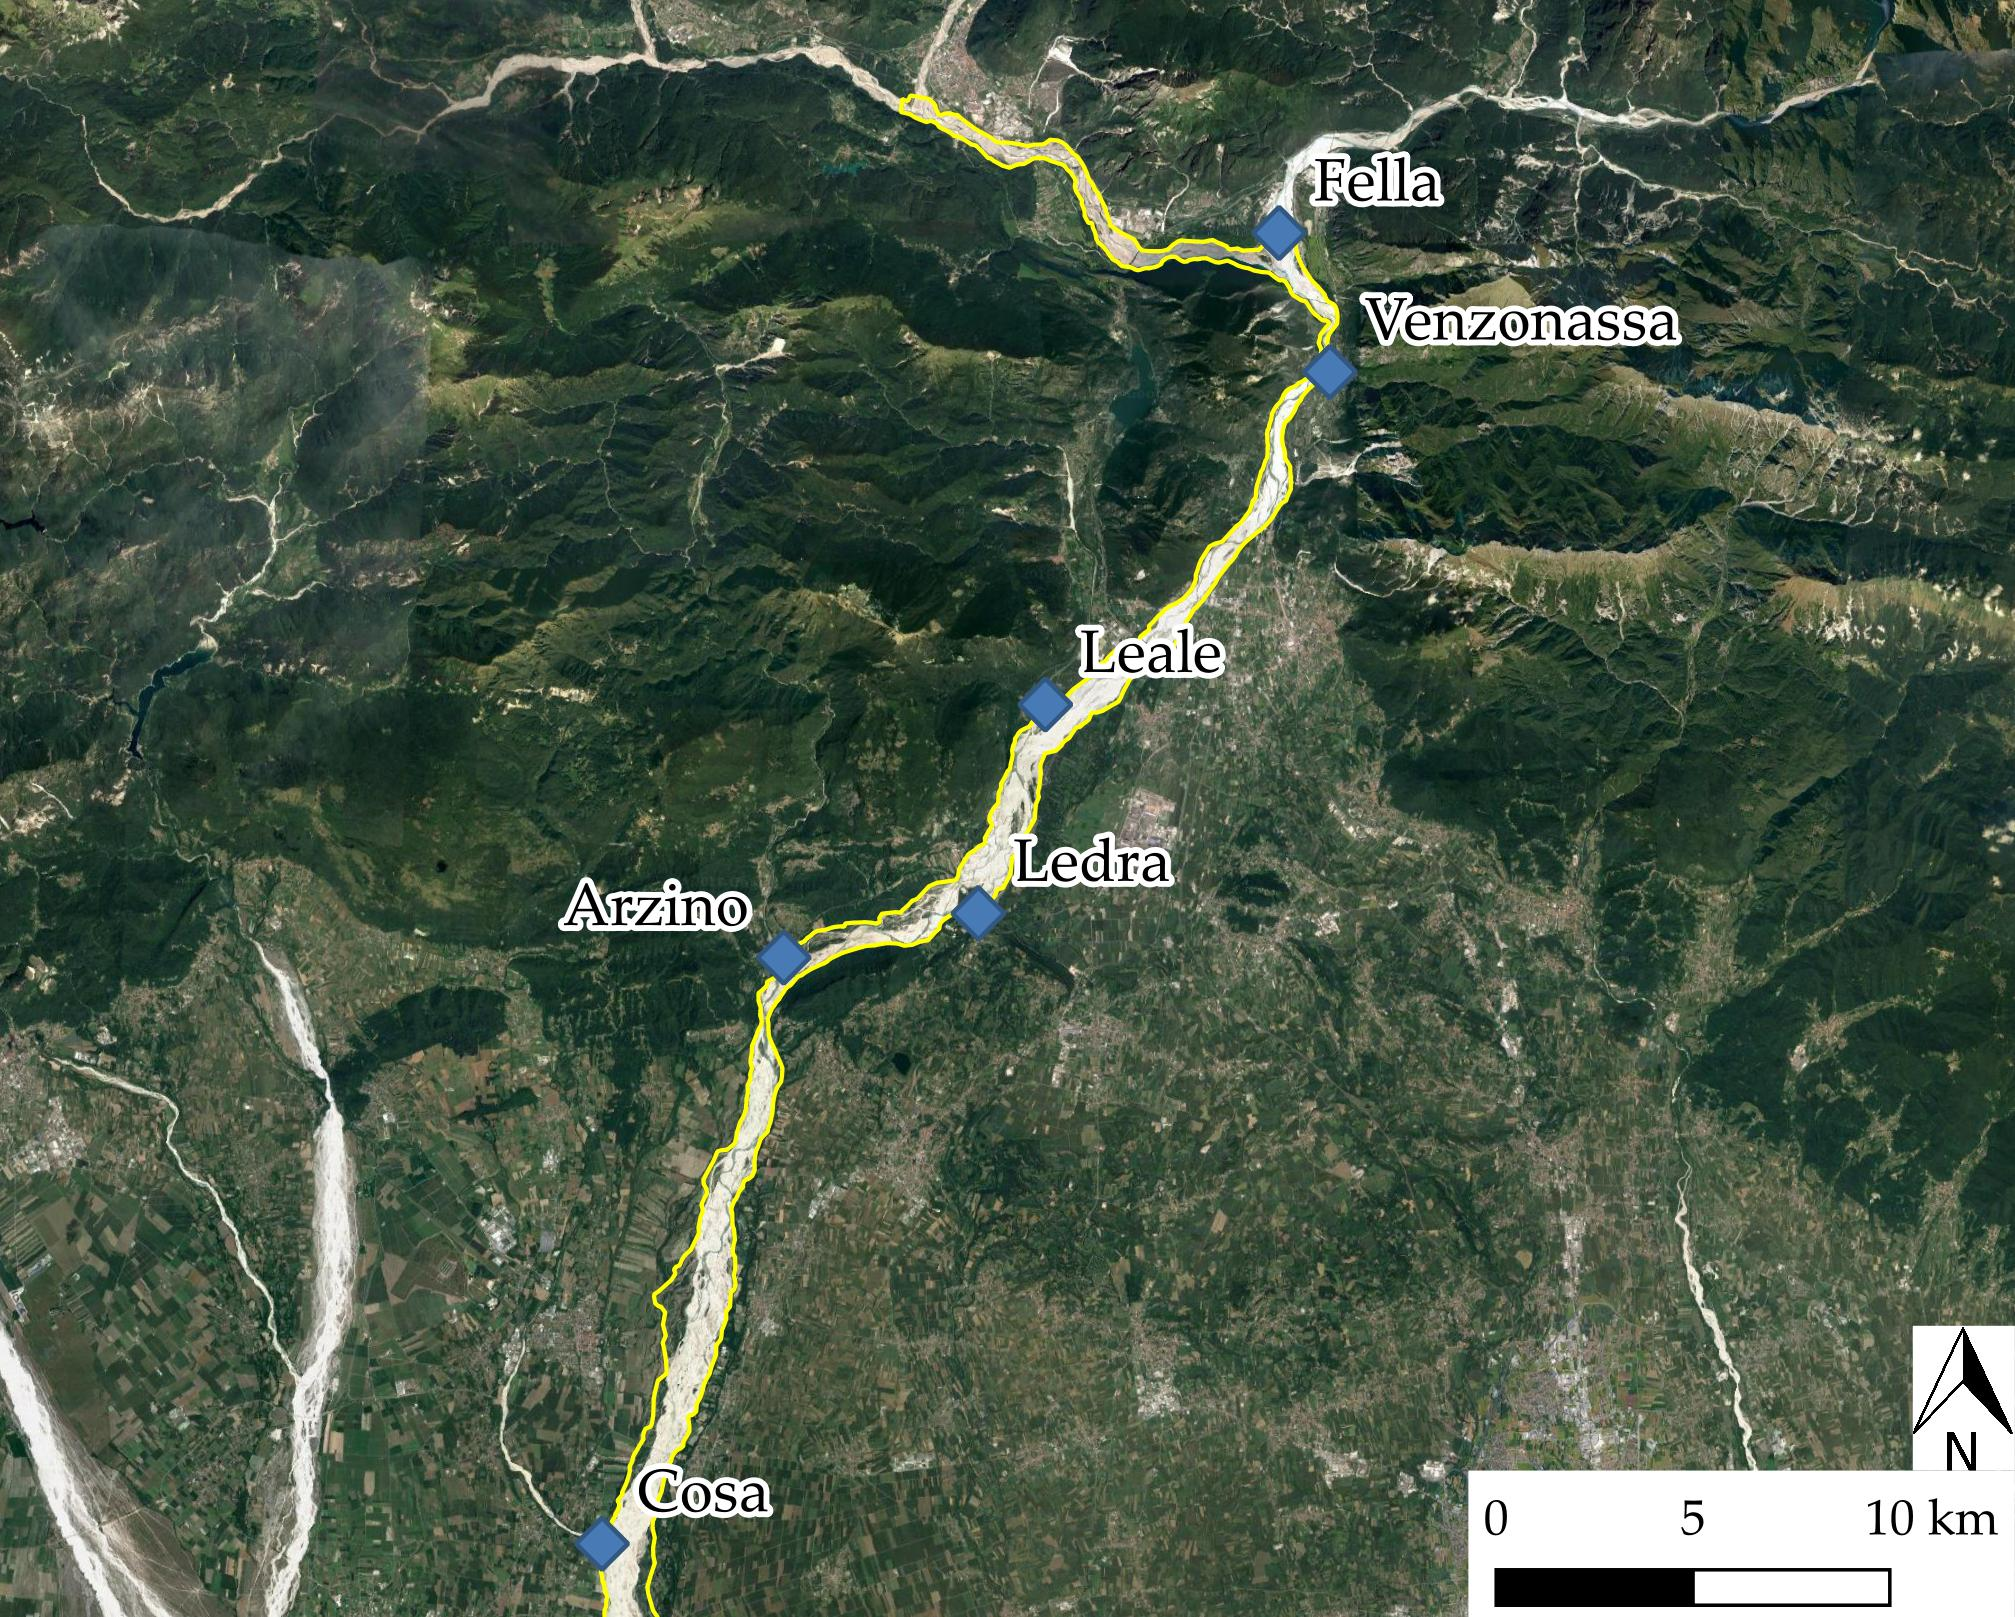
\includegraphics[width=\textwidth]{files/overview_affluenti.jpeg}
	\caption[principali affluenti nel tratto oggetto di studio]{principali affluenti nel tratto oggetto di studio (contornato in giallo); i rombi indicano i punti dove gli affluenti confluiscono nel Tagliamento.
	\\
	Map data: Google, Digital Globe.}
	\label{fig:affluenti}
\end{figure}
%
Il contributo di questi affluenti in termini di portata non è trascurabile; qualche decennio fa è stata evinta una relazione empirica tra l'area drenante di ogni bacino del Friuli Venezia Giulia \si{[\m\tothe{2}]} e la portata massima registrata in alcuni anni prima del 1950 \si{[\m\tothe{3}\per\s]} \squarecite{Mosetti:1983} che mostra l'evidente importanza degli affluenti:
%
\begin{equation}
	\label{eq:area-portata-mosetti}
	Q = 0.04598 \, A^{0.9546}	\quad	.
\end{equation}
%
Il limite di tale formula risiede nella determinazione delle portate utilizzate per la sua taratura; tuttavia la relazione fornisce la chiara indicazione che la portata in una sezione è all'incirca proporzionale all'area drenante sottesa.
\\
Si ritiene pertanto che conoscere il livello d'acqua in un punto del Tagliamento sia sufficientemente rappresentativo per descrivere qualitativamente l'entità di una piena in tutto il tratto di studio; per ottenere informazioni quantitative sulla portata fluente durante eventi di piena si assume che questa sia proporzionale all'area drenante in ogni sezione del fiume.

\paragraph{Dinamiche vegetazionali}
Nel fiume sono presenti numerose isole, composte prevalentemente da ontani bianchi \emph{Alnus incana} nei tratti montani (oltre l'area di studio), pioppi \emph{Populus nigra} e numerose specie di salice \emph{Salix spp.} nei tratti intermedi e vallivi.
Un'isola è un'area discreta e ben definita dell'alveo ricoperta da vegetazione e circondata da ghiaia o da canali (\cref{fig:esempio-isola}) \squarecites{Gurnell:2001-island-formation}{Bertoldi:2009-2m}.
%
\begin{figure}
	\centering
	\begin{subfigure}[b]{0.37\textwidth}
		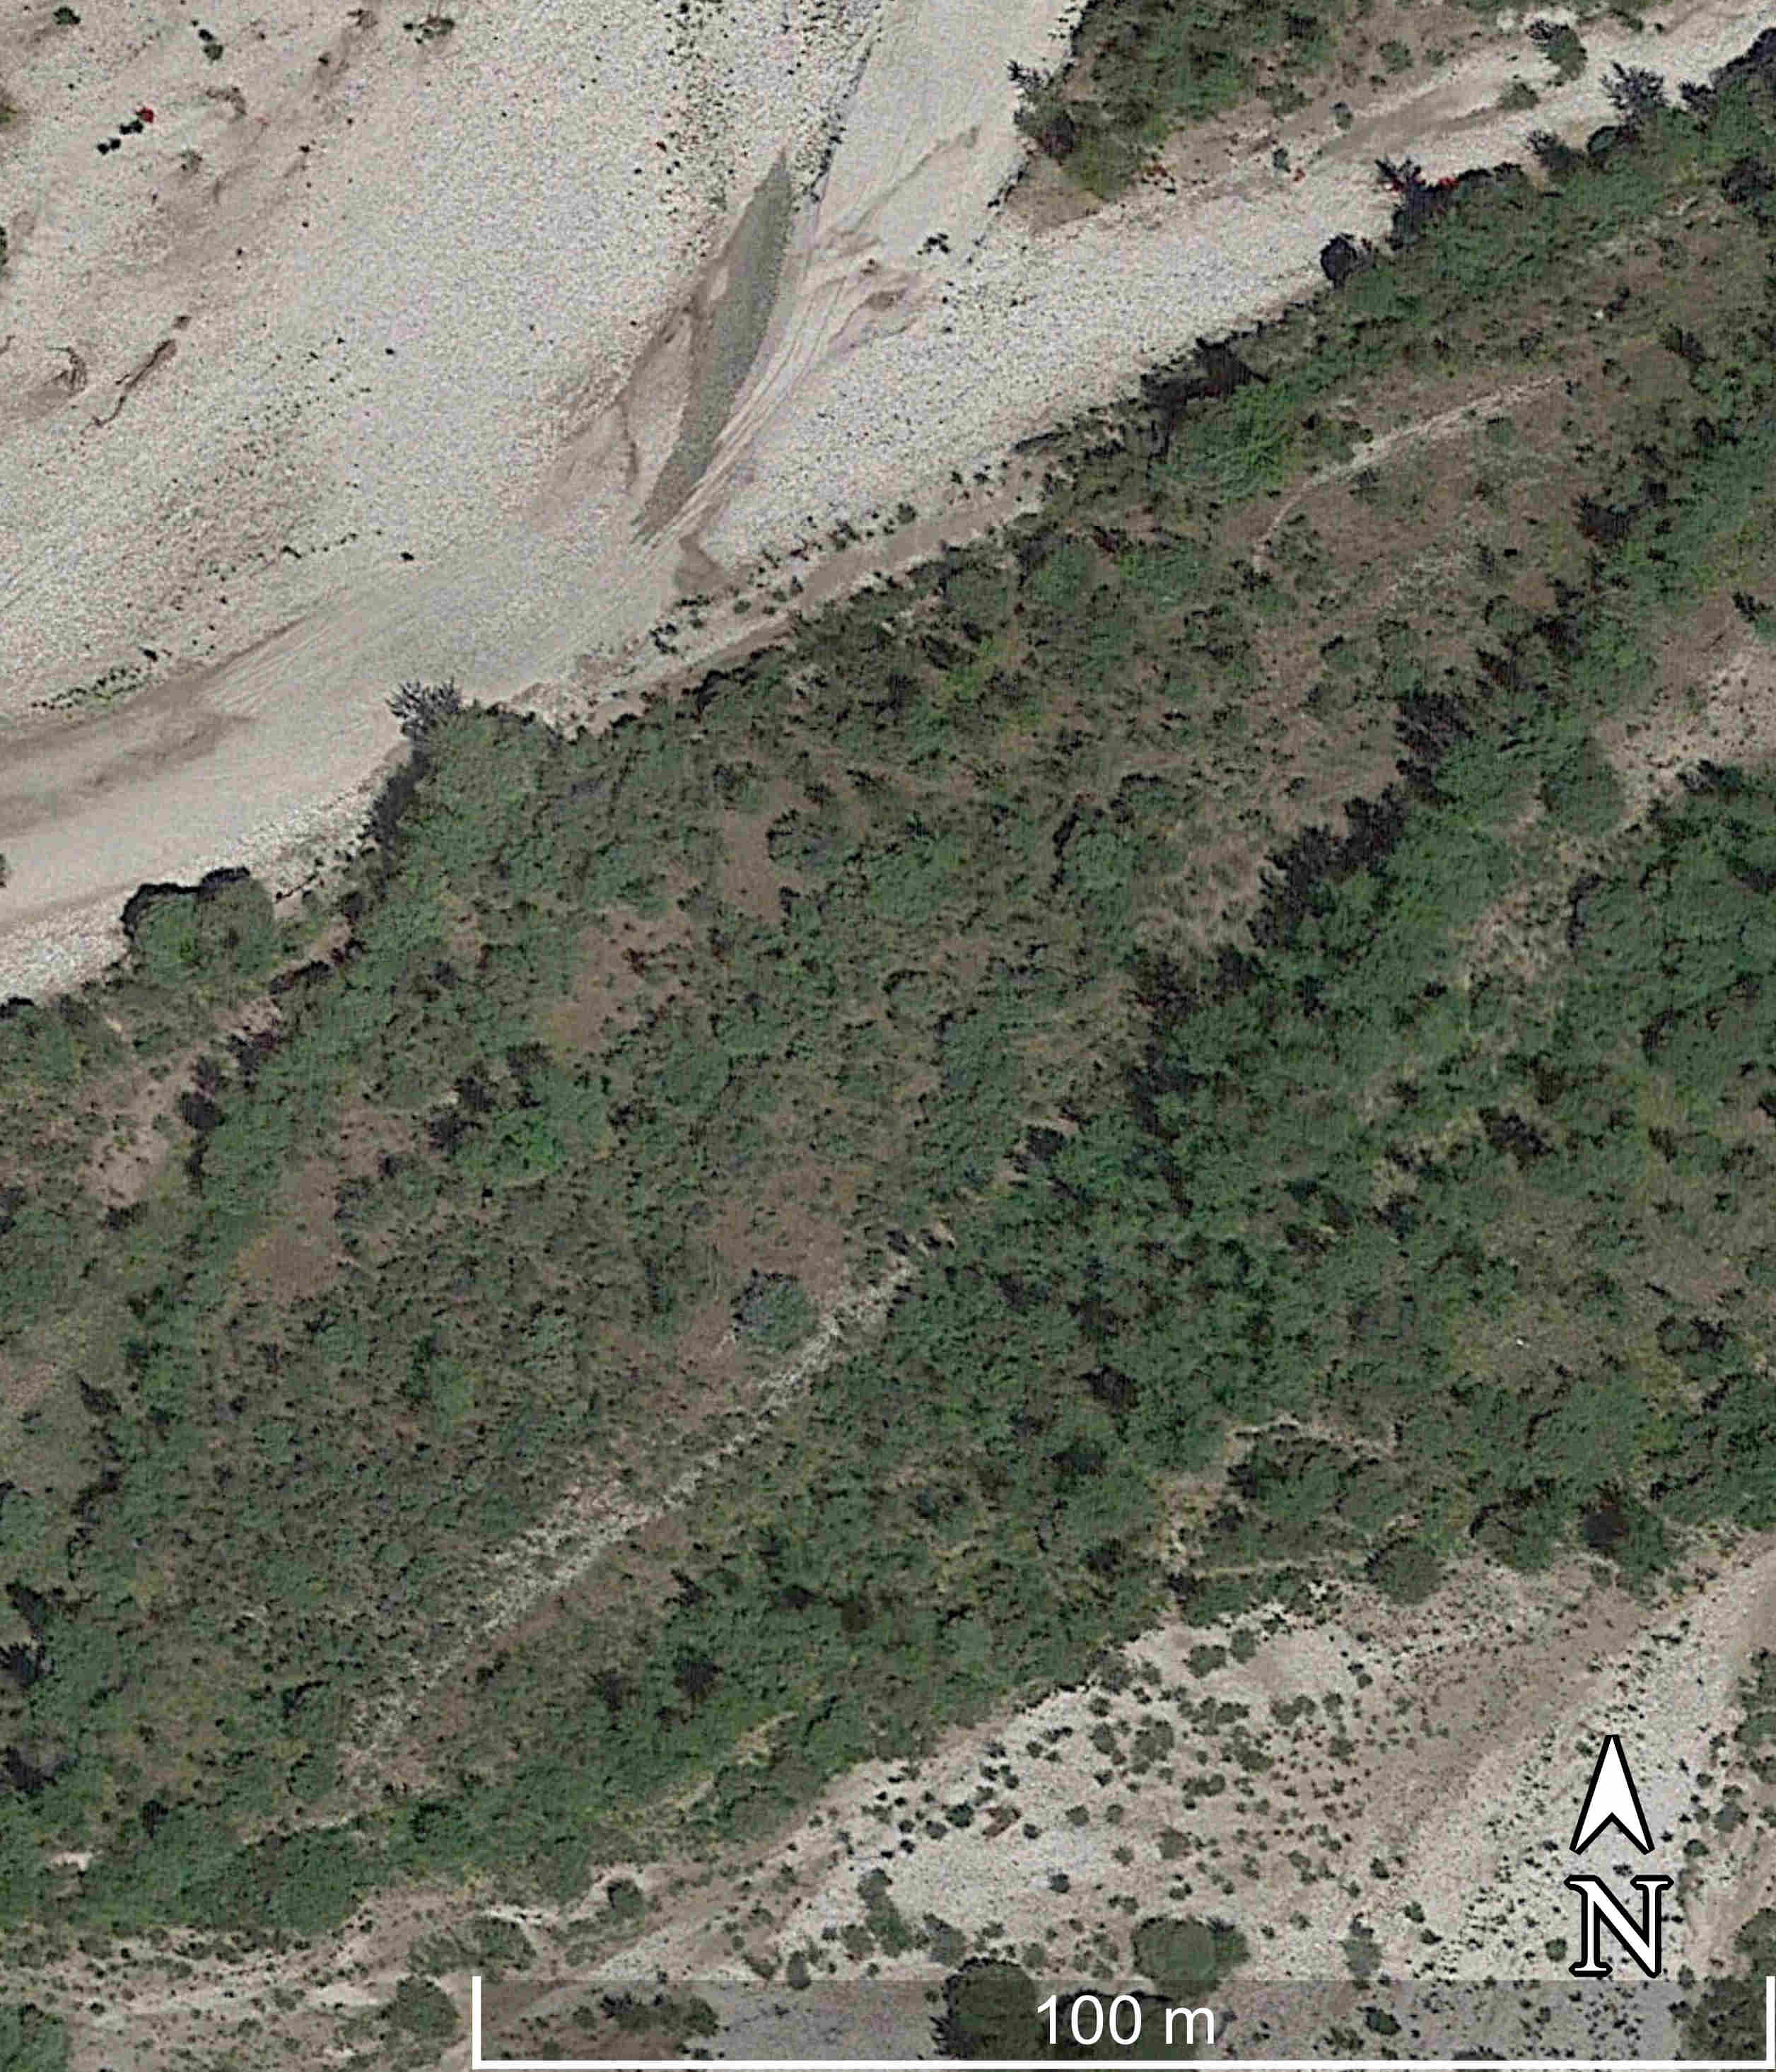
\includegraphics[width=\textwidth]{files/esempio_isola_sat_1.jpg}
	\end{subfigure}
	\quad
	\begin{subfigure}[b]{0.57\textwidth}
		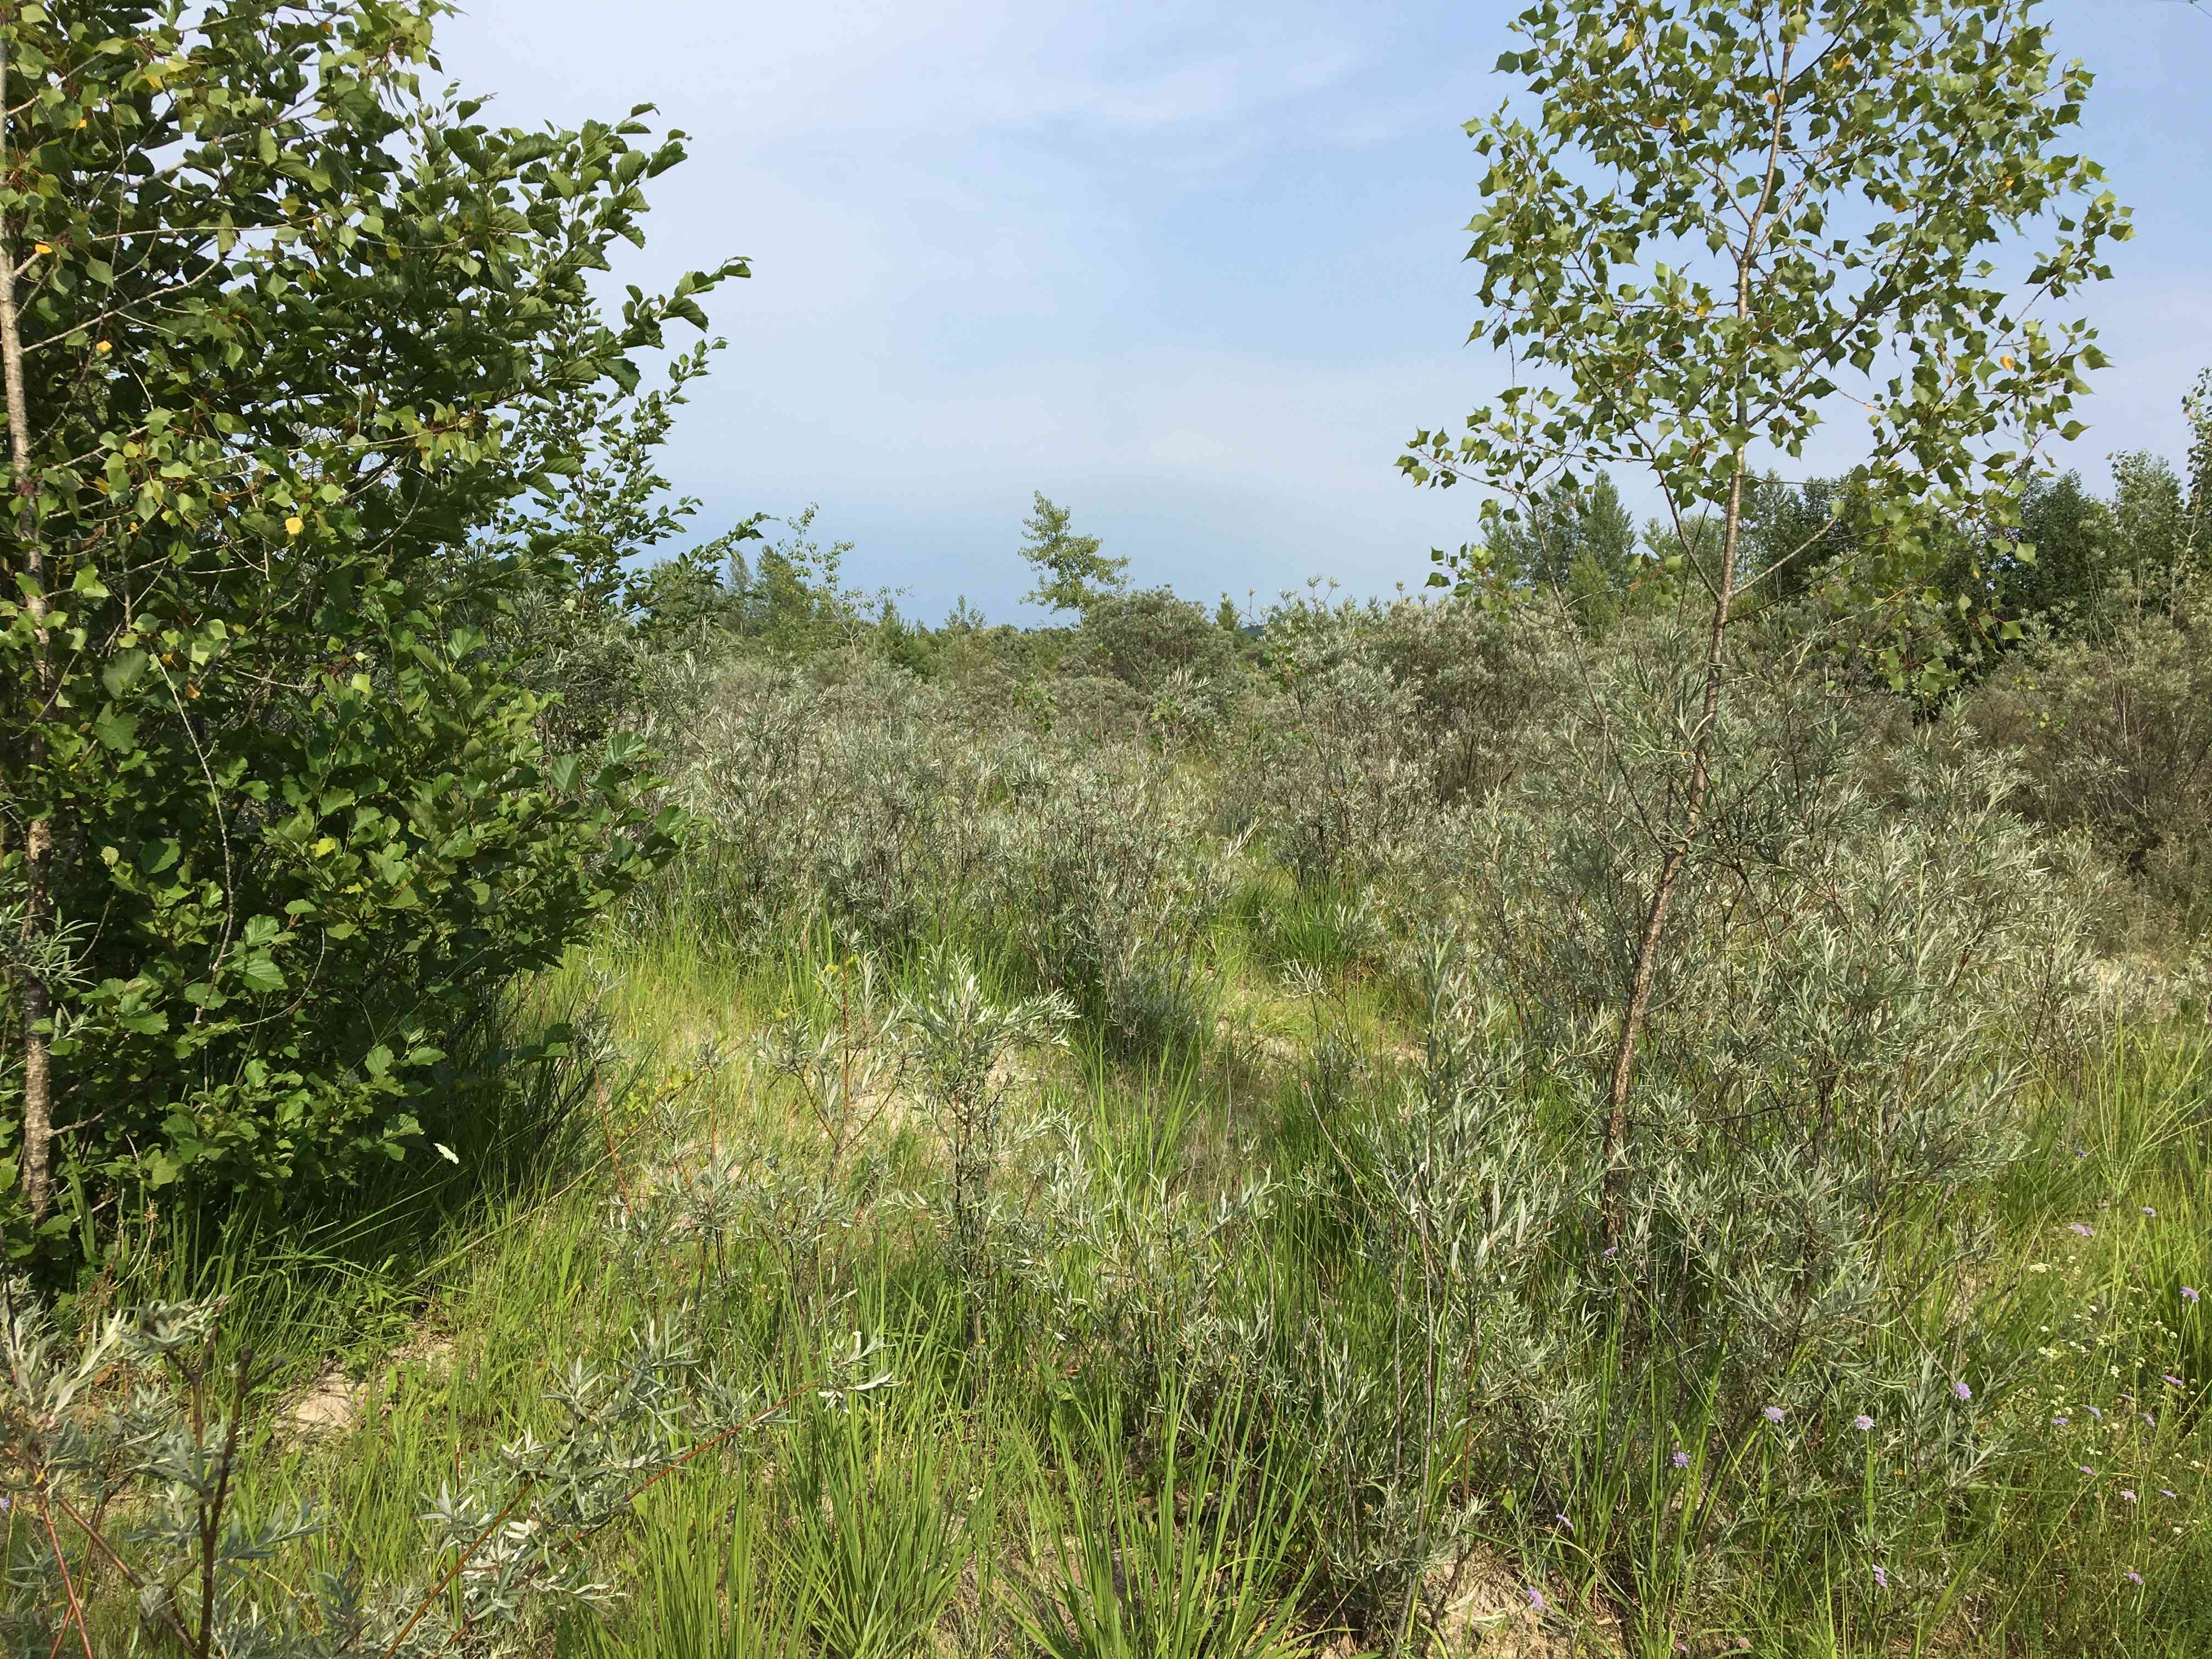
\includegraphics[width=\textwidth]{files/esempio_isola_1.jpg}
	\end{subfigure}
	\caption[immagine e foto di isole fluviali]{immagine da Google Earth e foto di isole fluviali; si noti la forte presenza di salici (\emph{Salix spp.}) e di pioppi (\emph{Populus nigra}); il luogo della foto è prossimo a quello dell'immagine.}
	\label{fig:esempio-isola}
\end{figure}
%
\\
Il meccanismo fondamentale di generazione di forme vegetate in alveo è la ricrescita vegetativa che caratterizza \emph{P. nigra} e \emph{Salix spp.}: i tronchi eradicati e trasportati dalle piene e in seguito depositati sulla nuda ghiaia rigettano rami e foglie (\cref{fig:esempio-accumulo});
se vi è la contemporaneità di adeguate condizioni ambientali (non eccessiva velocità di abbassamento della falda in un substrato di pezzatura adeguata) ed idrologiche (frequenti piene di piccola-media entità, chiamate \emph{flow pulses}) allora i tronchi vivi crescono, intrappolano sedimenti e creano un buon ambiente per la successiva colonizzazione da parte di nuove piante (isole pioniere);
le isole si aggradano (fino a \SI{2}{\m} \squarecite{Gurnell:2006-omega}) e accrescono caratterizzandosi con piante di diversa età (\emph{building island} e isole complesse) \squarecite{Gurnell:2001-island-formation}.
A loro volta la presenza delle isole influenza la posizione, grandezza, forma dei canali e le dinamiche del fondo.
%
\begin{figure}
	\centering
	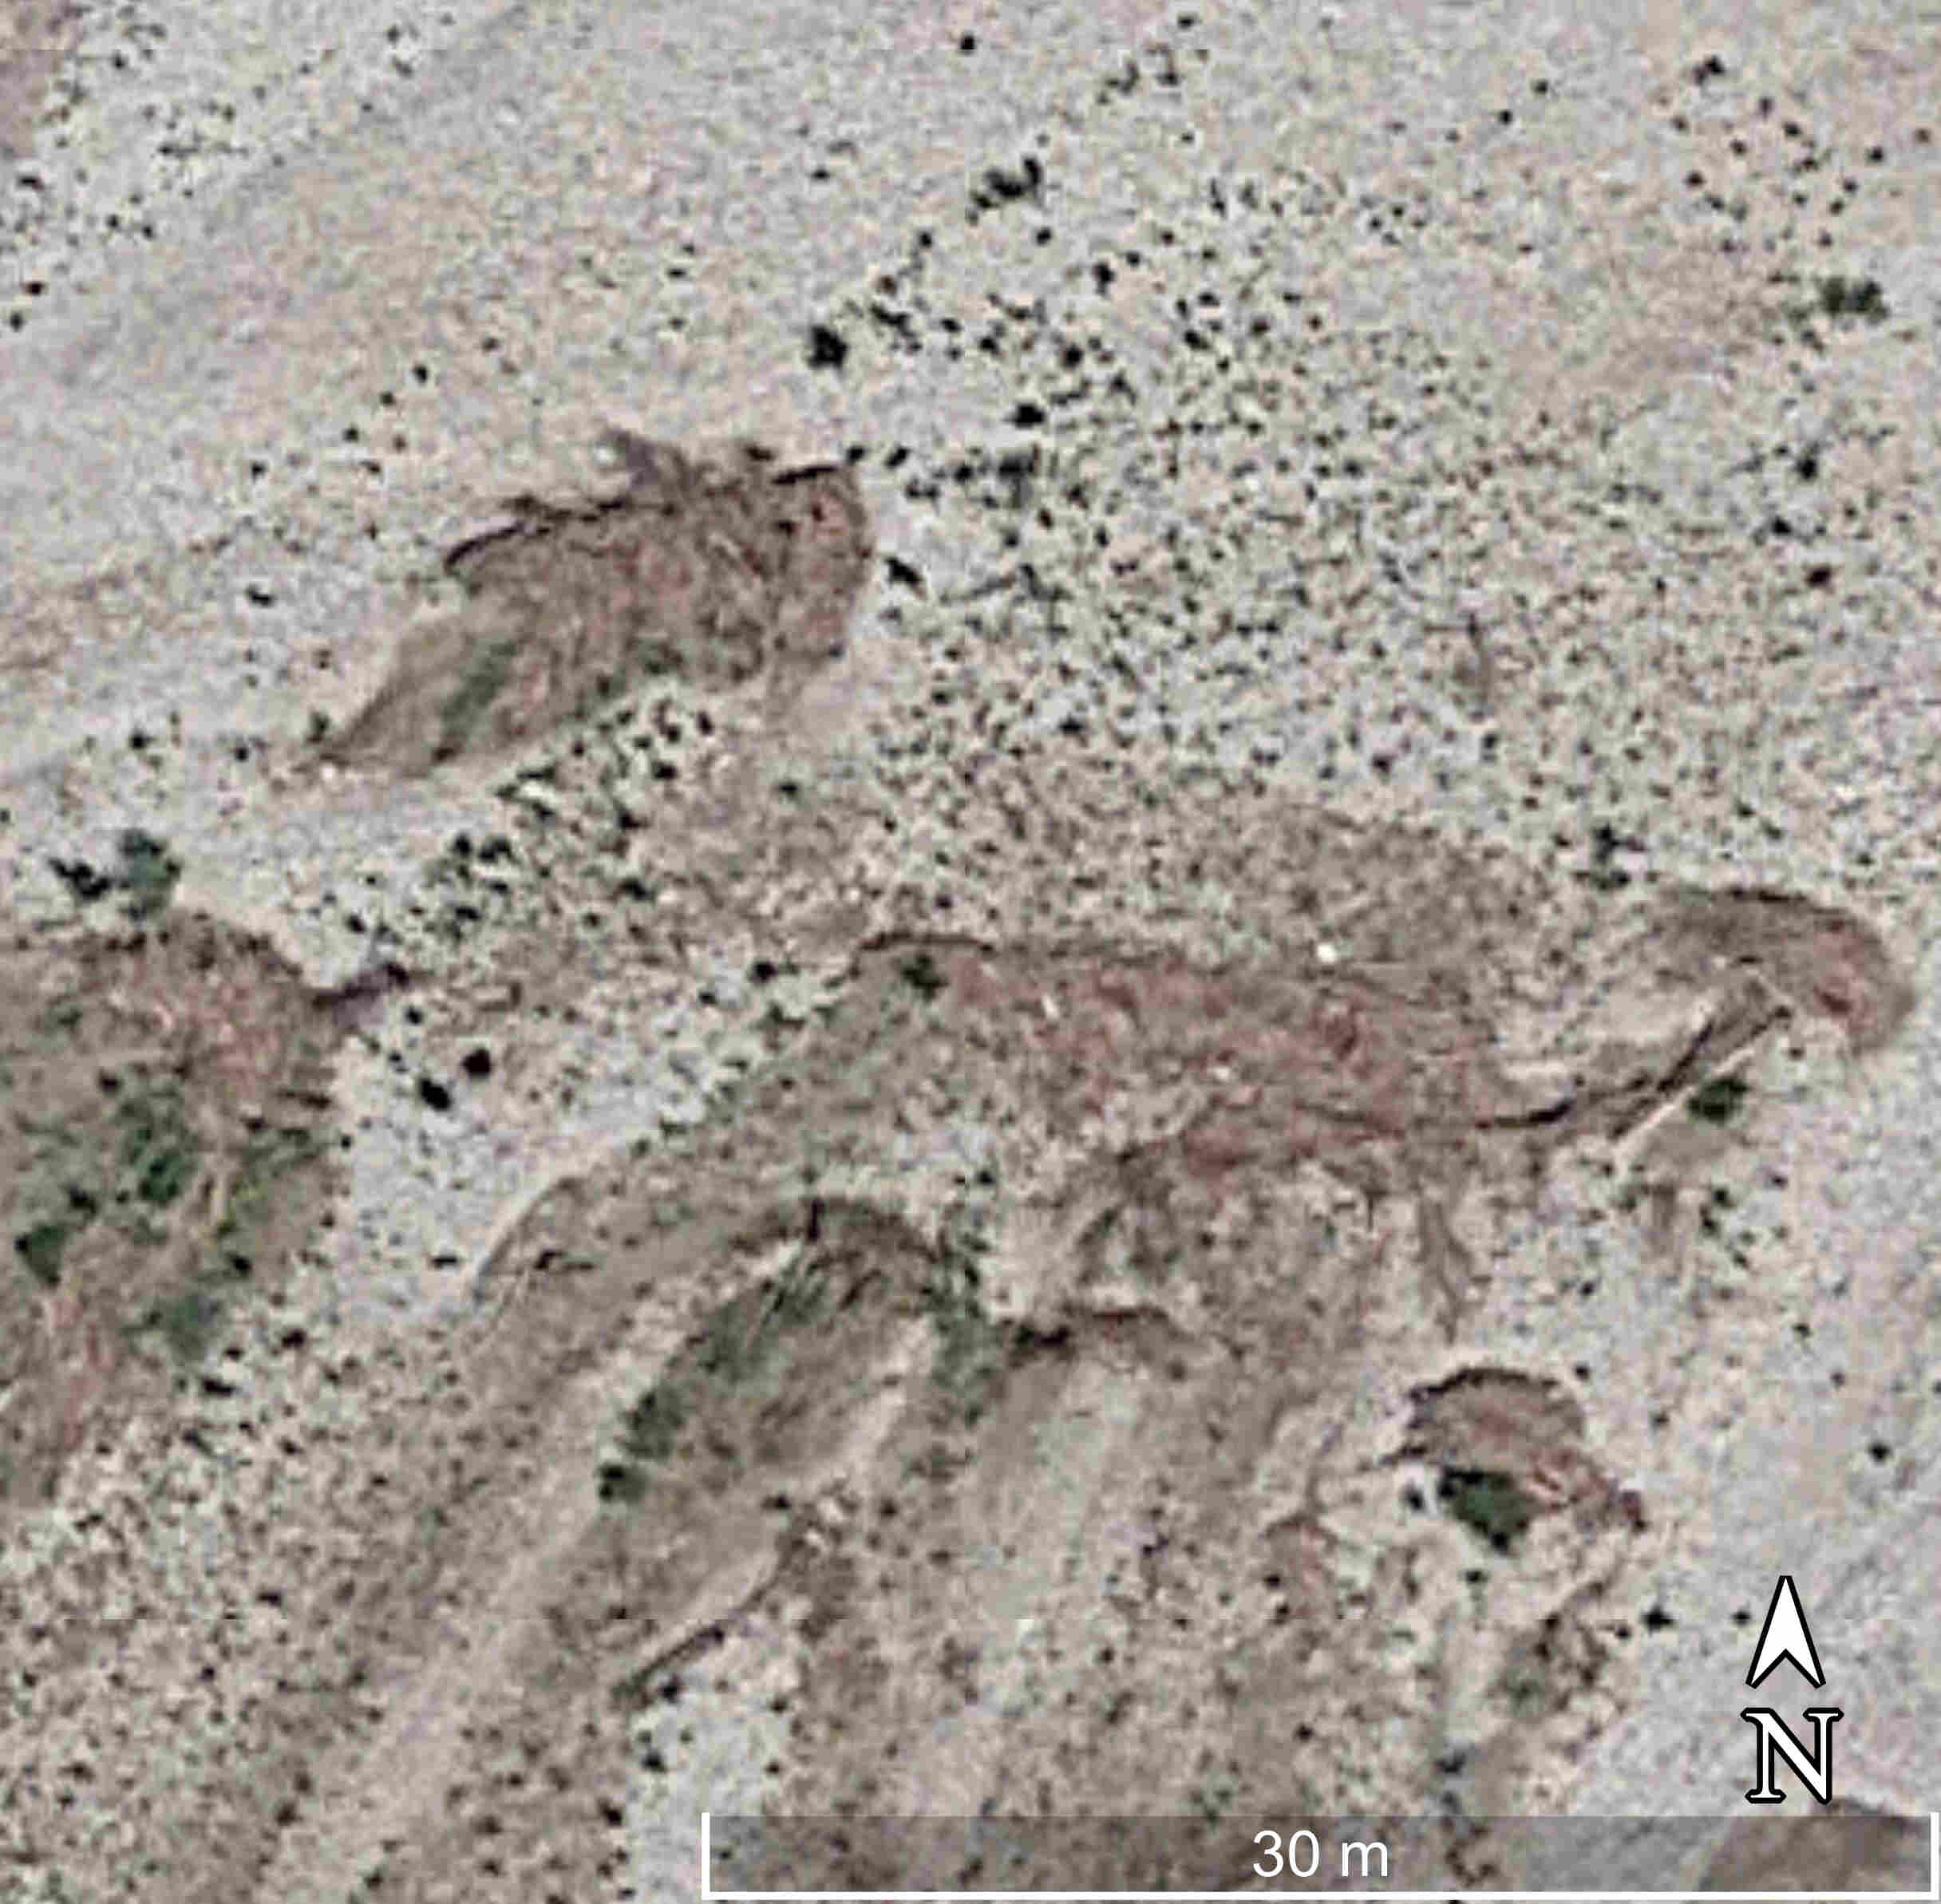
\includegraphics[width = .45\textwidth]{files/esempio_accumulo_sat_1.jpg}
	\quad
	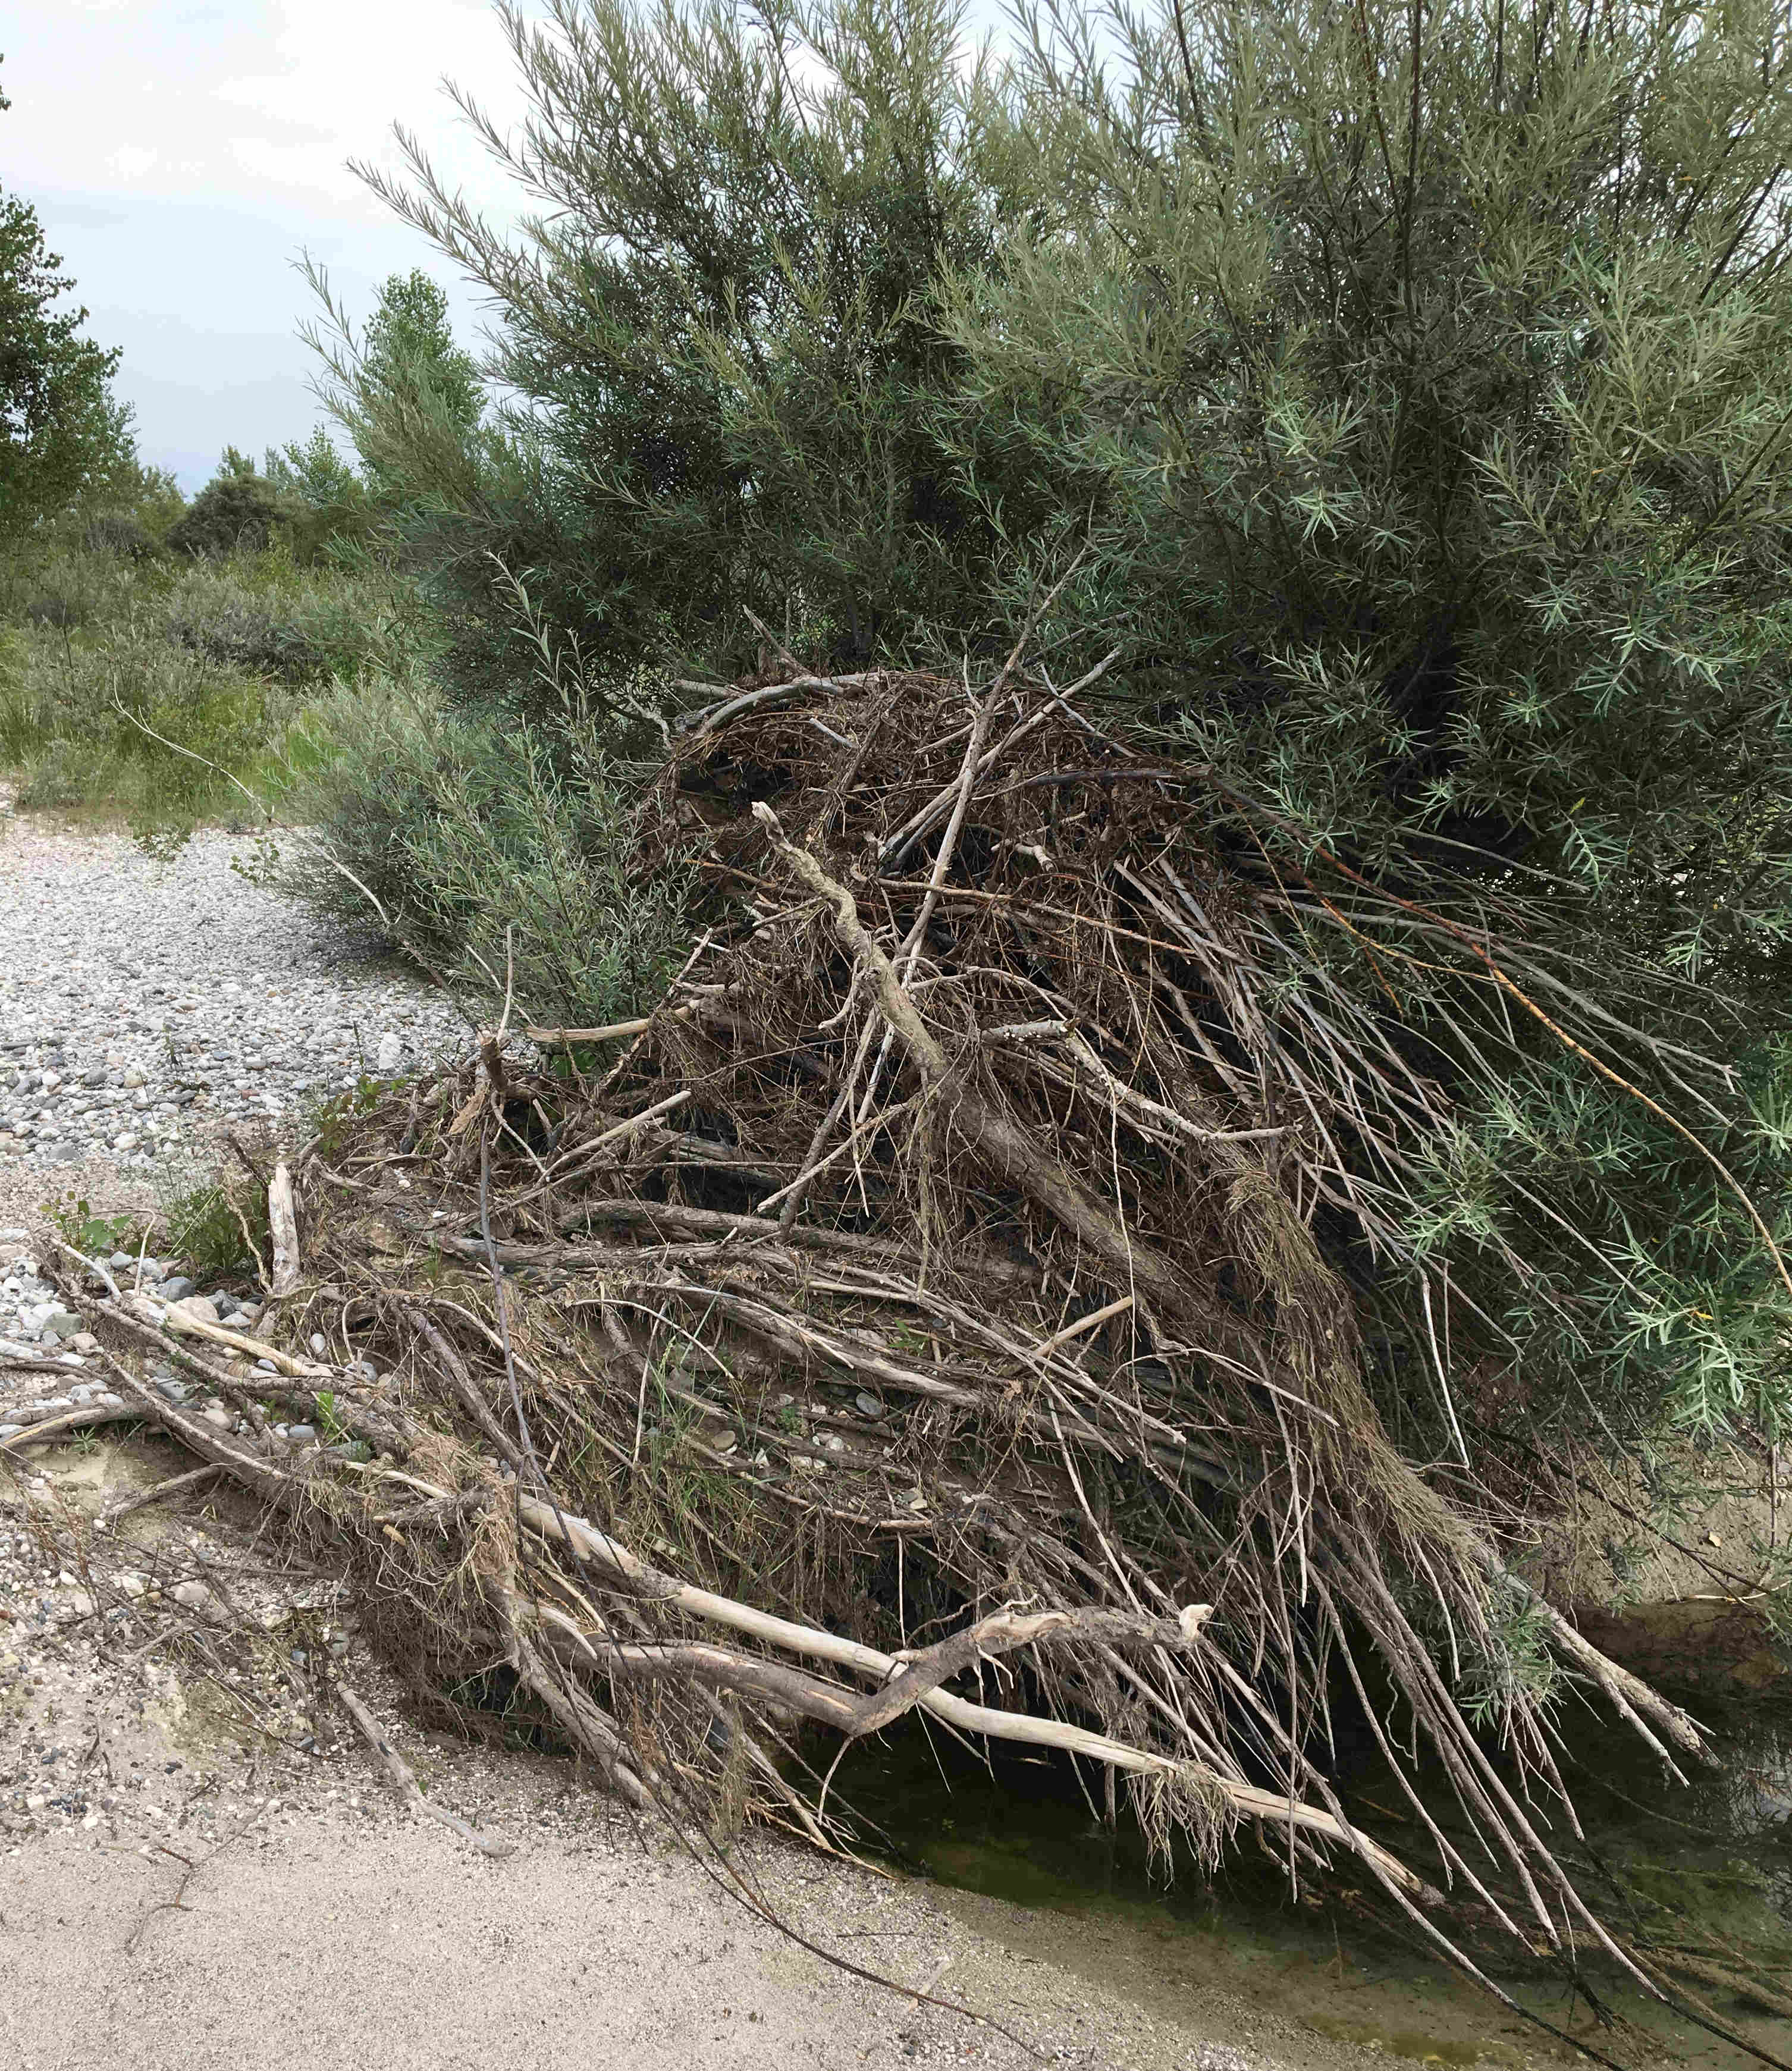
\includegraphics[width = .45\textwidth]{files/esempio_accumulo_1.jpg}
	\caption[immagine e foto di accumuli legnosi]{immagine da Google Earth e foto di accumuli legnosi in grado di rigettare nuovi rami e radici. Il luogo della foto non corrisponde a quello dell'immagine.}
	\label{fig:esempio-accumulo}
\end{figure}
%
\\
Si parla quindi di successione biogeomorfica nel corridoio fluviale attivo: l'ambiente fisico influenza la crescita delle piante coevolute con l'ambiente fluviale; queste a loro volta influenzano l'ambiente fisico e la sua evoluzione, tanto da essere state chiamate “ingegneri ecosistemici” \squarecites{Gurnell:2006-omega}{Gurnell:2014-plants-eng}.

Possono formarsi isole anche da piante nate da seme, anche se queste sono più esigenti in termini di condizioni ambientali ed idrologiche.
\\
Eventi di piena che riempiono l'alveo fino a lambire le sponde (\emph{bankfull}) od eventi più intensi possono dividere parti di vegetazione riparia dalla piana alluvionale, dando origine ad isole composte da piante mature coetanee, strutturalmente ben diverse dalle isole disetanee formate a partire da frammenti vegetativi.

Le isole sono distribuite disomogeneamente da monte verso valle: si può osservare che nei tratti con \emph{upwelling} il loro numero e la velocità di espansione crescono grazie all'acqua che risale dalla falda, mentre nei tratti con \emph{downwelling} la loro presenza diminuisce;
inoltre, nelle zone particolarmente più strette come nei tratti montani o presso la stretta di Pinzano l'intensità della corrente è tale da ridurre o inibire la crescita di vegetazione, come mostrato da un modello concettuale in letteratura \squarecite{Gurnell:2014-plants-eng}.
\\
Temporalmente, le uniche isole che non vengono erose sono quelle che si fondono nella piana alluvionale; anche isole insediatesi da anni in alveo, aggradatesi fino a porsi a quote simili a quelle della \emph{floodplain}, possono essere completamente spazzate durante eventi \emph{bankfull} o maggiori.
Difatti è stato mostrato che la maggior parte delle isole nel tratto compreso tra il ponte autostradale di Braulins e la stretta di Pinzano persistono meno di \SI{24}{\anni} \squarecite{Zanoni:2008}; risultati simili sono stati presentati per un tratto nei pressi di San Paolo~(PN), corrispondente ai tratti più a valle nella presente tesi \squarecite{Bertoldi:2009-2m}.

L'isola presente nel tratto~9 (\cref{fig:23-tratti}), nei pressi di Cornino, si fonda su un nucleo roccioso.
Questa isola non è soggetta alle dinamiche tipiche delle isole che crescono sulla ghiaia dell'alveo: nemmeno le piene più intense possono asportarla od eroderla parzialmente.


\section{Stato dell'arte ed obiettivi}
\label{sec:stato-arte-obiettivi}
L'obiettivo principale della presente tesi è lo studio delle dinamiche delle isole nel Tagliamento in risposta al regime idrologico (successione di magre, morbide, piene) e la comprensione dei fattori che controllano le traiettorie evolutive della vegetazione.
In via previsionale si cerca di rispondere all'esigenza di stimare in anticipo gli effetti che una piena può avere sulle isole, risultato che aiuterebbe anche a migliorare la gestione dei fiumi e della vegetazione presente in essi in altri contesti dove le portate sono regolate dall'uomo. 
\\
Lo studio è stato effettuato su un periodo di 18~anni, dal~2000 al~2018, analizzando dati telerilevati con tecniche diverse (immagini satellitari, foto aeree, rilievi aerei topografici LiDAR).
I dati così ottenuti sono stati messi in relazione al regime idrologico dello stesso periodo, caratterizzato dalle misure idrometriche di livello del pelo libero presso la stazione di Villuzza~(UD). 

Articoli precedentemente pubblicati hanno studiato l'ecologia e la morfodinamica del Tagliamento, le interrelazioni tra piante e fiume, la crescita della vegetazione riparia, la localizzazione delle isole in questo contesto naturale e molto altro.
\\
Alcuni lavori si sono basati su immagini aeree e indagini di campo \squarecites{Zanoni:2008}{Bertoldi:2010-d50}{Surian:2015}: da una parte questi permettono la raccolta di informazioni in grande dettaglio, ma con risoluzione spaziale modesta (i rilievi aerei hanno un costo non indifferente) e risoluzione temporale particolarmente limitata (da pochi anni a decenni tra ogni rilievo).
\\
L'utilizzo di immagini satellitari multitemporali a bassa risoluzione permette di avere una visione d'insieme dei fenomeni, così come di evidenziare differenze spaziali e temporali.
Infatti è già stato dimostrato che è possibile estrarre risultati significativi sulla vegetazione riparia e sulle sue dinamiche da immagini satellitari a bassa risoluzione \squarecites{Bertoldi:2011-ASTER}{Henshaw:2013-LandSat}.
Questi lavori tuttavia hanno utilizzato delle maschere fisse per delimitare l'area attiva, senza distinguere in ogni immagine le isole dalla \emph{floodplain}.
\\
Alcuni autori hanno inoltre formulato modelli concettuali sulle dinamiche vegetazionali nei fiumi, in particolare nel Tagliamento \squarecites{Gurnell:2001-island-formation}{Gurnell:2006-omega}{Gurnell:2014-plants-eng}.
\\
Generalmente, il tratto più frequentemente studiato è quello compreso tra il ponte autostradale di Braulins~(UD) e la stretta di Pinzano.

Con la presente tesi si vuole provare a rispondere alle seguenti domande, anche grazie ai risultati ottenuti in lavori precedenti.
%
\paragraph{Quante isole sono presenti e cosa ne regola la presenza?}
La larghezza media dell'alveo e la percentuale di isole rispetto all'alveo attivo sono state due grandezze studiate per caratterizzare spazialmente e temporalmente il Tagliamento:
%
\begin{itemize}
	\item il tracciamento della traiettoria evolutiva della larghezza ha permesso di vedere come il tratto a monte di Pinzano si sia ristretto negli ultimi due secoli di più del \SI{50}{\percent}, mentre a partire dalla fine del~1900 sembra che l'alveo abbia ripreso un processo di allargamento \squarecites{Zanoni:2008}{Surian:2015};
	gli autori suggeriscono che il restringimento possa essere dovuto alla concomitanza di lievi cambiamenti naturali nel regime delle portate e per l'estrazione di ghiaia dall'alveo per scopi civili negli anni '70 e '80 del secolo scorso, come è avvenuto per altri fiumi simili \squarecite{Sitzia:2016-d50};
	le cause dell'allargamento possono essere il veto all'estrazione della ghiaia congiuntamente ad un periodo caratterizzato da piene intense nei primi anni del 2000;
	%
	%
	\item la proporzione tra isole e alveo attivo è stata considerata da più autori \squarecites{Zanoni:2008}{Bertoldi:2011-ASTER}{Henshaw:2013-LandSat}{Surian:2015}; 
	mentre alcuni risultati sembrano mostrare un rapporto oscillante attorno ad un valore medio di \SI{8}{\percent} \squarecite{Zanoni:2008}, altri mostrano valori abbastanza diversi come ordine di grandezza \squarecite{Henshaw:2013-LandSat} (probabilmente dovuti all'utilizzo di immagini satellitari con celle di \SI{30}{\m}) o con un trend temporale opposto rispetto alla larghezza \squarecite{Surian:2015}.
\end{itemize}	
%
In un modello concettuale presentato pochi anni fa viene proposta la potenza della corrente come fattore che regola la presenza delle isole \squarecite{Gurnell:2006-omega}: se la corrente ha mediamente un'elevata energia per unità di larghezza, allora la crescita delle piante è inibita; se la potenza è inferiore ad una soglia individuata dagli autori, allora la formazione ed espansione delle isole è controllata da altri fattori ambientali, come la quota della falda e la granulometria del substrato dove crescono le piante.

Con i dati di questa tesi è possibile estendere al periodo presente i risultati e le osservazioni effettuate dagli altri autori sulla larghezza e sulla proporzione di isole rispetto all'alveo attivo, così come sfruttare la maggior risoluzione temporale delle immagini per osservare cambiamenti avvenuti in periodi più brevi.
\\
Inoltre, si cerca non solo di verificare l'esistenza di un valore limite della potenza della corrente oltre il quale non crescono più isole, ma di capire se e in che misura questo fattore può influenzare la massima proporzione di isole presenti in alveo.

\paragraph{In quali condizioni e in quale misura cambiano le isole?}
Le isole sono soggette a continue dinamiche di erosione in seguito alle piene e di accrescimento nei periodi tra un evento e quello successivo.
\\
Diversi autori hanno considerato la persistenza media delle isole nell'alveo, dell'ordine di una ventina d'anni; gli stessi hanno quantificato anche la percentuale di isole erose e le nuove aree vegetate \squarecites{Zanoni:2008}{Bertoldi:2009-2m}{Bertoldi:2011-ASTER}{Surian:2015}.
Tuttavia in alcuni lavori la risoluzione temporale è particolarmente bassa (un'immagine ogni decina di anni), in altri il periodo di studio limitato a pochi anni; in tutti il tratto studiato era quello menzionato all'inizio della sezione, lungo circa~\SI{20}{\kilo\m}.
Si può quindi cercare di migliorare ed ampliare questi risultati sia da un punto di vista spaziale che temporale.
\\
La riproduzione vegetativa a partire da tronchi vivi depositati in alveo è uno dei principali meccanismi di formazione delle isole nel Tagliamento \squarecite{Gurnell:2001-island-formation}. 
Grazie alle ortofoto e alle immagini satellitari ad alta risoluzione si può osservare quanto legno è presente in alveo; con i rilievi LiDAR  si può controllare se gli elementi legnosi che non vengono mobilitati dalle piene sono quelli posti a quote relative maggiori; infine, si può cercare quanti tronchi e accumuli legnosi crescono fino a formare nuove isole.

\paragraph{È utile analizzare l'età delle isole?}
Alcuni autori hanno mostrato come la vegetazione riparia delle isole possa avere una diversa struttura di età in base alle modalità di accrescimento e come le piante mature possano essere generalmente più resistenti all'erosione di piante allo stadio iniziale della successione biogeomorfica \squarecites{Gurnell:2001-island-formation}{Gurnell:2014-plants-eng}.
\\
Ad oggi, tuttavia, sembra che nessun autore abbia provato a caratterizzare l'età della vegetazione nelle isole per migliorare risultati riguardo le dinamiche delle isole.
\\
Con questa tesi si prova ad implementare la divisione della vegetazione nelle isole in classi di età e a verificare se e quanto i risultati ne vengono influenzati: sono le piante più giovani quelle che possono essere erose più facilmente?

\paragraph{Qual è la relazione tra regime delle piene e dinamiche delle isole?}
Precedentemente è già stata formulata una relazione tra isole erose e portata \squarecite{Surian:2015};
questa tuttavia è basata su una piccola quantità di dati e non tiene conto dell'invecchiamento della vegetazione tra piene successive, fattore interessante poiché si potrebbe osservare un'erosione differenziata tra isole appena formatesi e isole insediate in alveo da anni.
\\
Riguardo l'accrescimento, al momento attuale non sono noti all'autore lavori che mettano in relazione la crescita della vegetazione con il periodo che intercorre tra piene successive.

\section{Convenzioni}
Le seguenti convenzioni saranno utilizzate nella presente tesi:
\begin{description}
	\item[Capitoli] riprendono le domande formulate nella sezione~\ref{sec:stato-arte-obiettivi}; ogni sezione di risposta è suddivisa in metodi (quali tecniche sono state utilizzate e quali analisi sono state svolte), risultati (cosa è possibile osservare oggettivamente dai dati) e discussione (quale interpretazione è possibile dare ai risultati);
	\item[Mappe] riportate secondo WGS84/UTM~33N (EPSG:~32633);
	\item[Direzione della corrente] riportata con una freccia blu nelle immagini;
	\item[Formato delle date] AAAA-MM-GG;
	\item[Citazioni] sono nel formato Autore/i-Anno, racchiuse tra parentesi quadre;
	\item[Web link] sono riportati in note a piè pagina;
	\item[Termini in lingua straniera] sono in corsivo;
	\item[Glossario] presente nel materiale finale.
	%
\end{description}


%----------------------------------------------------------



\chapter{Materiali e strumenti}
Nel presente capitolo viene inizialmente introdotta l'entità fisica a fondamento di tutto il lavoro: la radiazione elettromegnetica;
in seguito vengono riportati i materiali da cui sono stati estratti i dati per le analisi e gli strumenti utilizzati nelle elaborazioni.


\section{La radiazione elettromagnetica}
Gli strumenti di acquisizione di immagini aeree e satellitari sono sensibili a determinate lunghezze d'onda della radiazione elettromagnetica (\cref{graph:el-mag-radiation}), cioè sono in grado di registrarne solo alcune porzioni (bande).
L'occhio umano può distinguere solo le bande del visibile, mentre i sensori artificiali possono acquisire altre bande della radiazione.
%
\begin{figure}
	\centering
	\tikzsetnextfilename{electromagnetic_radiation}
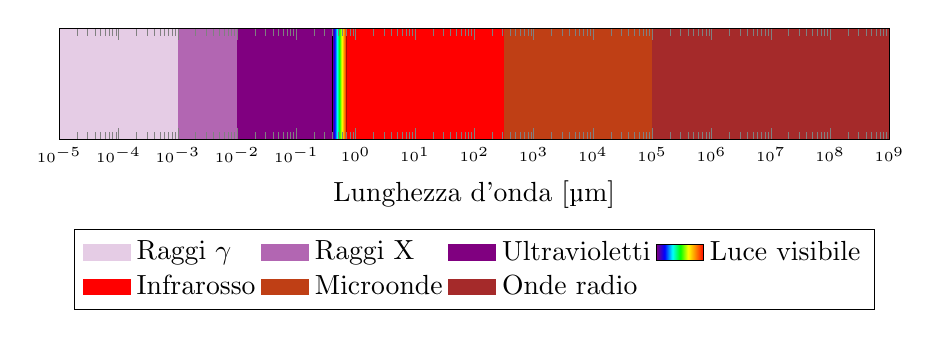
\begin{tikzpicture}[fill between/on layer={axis grid}]
	\begin{axis}[
		xlabel={Lunghezza d'onda},
		xticklabel style = {font=\tiny,yshift=0.2ex},
		xmin=10^-5,
		xmax=10^9,
		x unit=\si{\micro\meter},
		xmode=log,
		ymin=0,
		ymax=1,
		height=3cm,
		width=\textwidth,%12.2cm,
		yticklabels={},
		ytick=\empty,
		legend cell align=left,
		legend style={
			at={(0.5,-0.8)},%(0.85,-0.77)},
			anchor=north,
			legend columns=4,
			}
	]
	\addplot[draw=none, name path=start, forget plot] coordinates{(10^-5,0)(10^-5,1)};
	\addplot[draw=none, name path=gamma, forget plot] coordinates{(10^-3,0)(10^-3,1)};
	\addplot[draw=none, name path=xrays, forget plot] coordinates{(10^-2,0)(10^-2,1)};
	\addplot[draw=none, name path=uv, forget plot] coordinates{(0.4,0)(0.4,1)};
	\addplot[draw=none, name path=visible, forget plot] coordinates{(0.7,0)(0.7,1)};
	\addplot[draw=none, name path=ir, forget plot] coordinates{(10^2.5,0)(10^2.5,1)};
	\addplot[draw=none, name path=microwave, forget plot] coordinates{(10^5,0)(10^5,1)};
	\addplot[draw=none, name path=radiowave, forget plot] coordinates{(10^9,0)(10^9,1)};
	\addplot[violet!20, area legend] fill between[of=start and gamma];
	\addlegendentry{Raggi $\gamma$}
	\addplot[violet!60, area legend] fill between[of=gamma and xrays];
	\addlegendentry{Raggi X}
	\addplot[violet, area legend] fill between[of=xrays and uv];
	\addlegendentry{Ultravioletti}
	\addplot[shading=visiblelight, area legend] fill between[of=uv and visible];
	\addlegendentry{Luce visibile}
	\addplot[red, area legend] fill between[of=visible and ir];
	\addlegendentry{Infrarosso}
	\addplot[Bittersweet, area legend] fill between[of=ir and microwave];
	\addlegendentry{Microonde}
	\addplot[Brown, area legend] fill between[of=microwave and radiowave];
	\addlegendentry{Onde radio}
	\end{axis}
\end{tikzpicture}

	\caption[la radiazione elettromagnetica]{la radiazione elettromagnetica con le sue lunghezze d'onda.}
	\label{graph:el-mag-radiation}
\end{figure}
%
\\
Le immagini nel visibile sono solitamente suddivise nelle bande del Rosso, Verde e Blu (\emph{Red}, \emph{Green}, \emph{Blue}, R-G-B); ognuna indica la quantità di colore presente; la combinazione di queste quantità di colore restituisce l'immagine a colori.
\\
Per poter osservare immagini con bande diverse dal visibile si sostituisce una o più bande R-G-B con le bande in questione.
Ad esempio, è possibile sostituire la banda del Rosso con quella dell'Infrarosso (IR): la quantità di colore del Rosso sarà rimpiazzata dalla quantità di colore dell'Infrarosso.
Il risultato sarà un'immagine riconoscibile dall'occhio umano, ma in falsi colori (\cref{fig:confronto-bande-intro}).
%
\begin{figure}
	\centering
	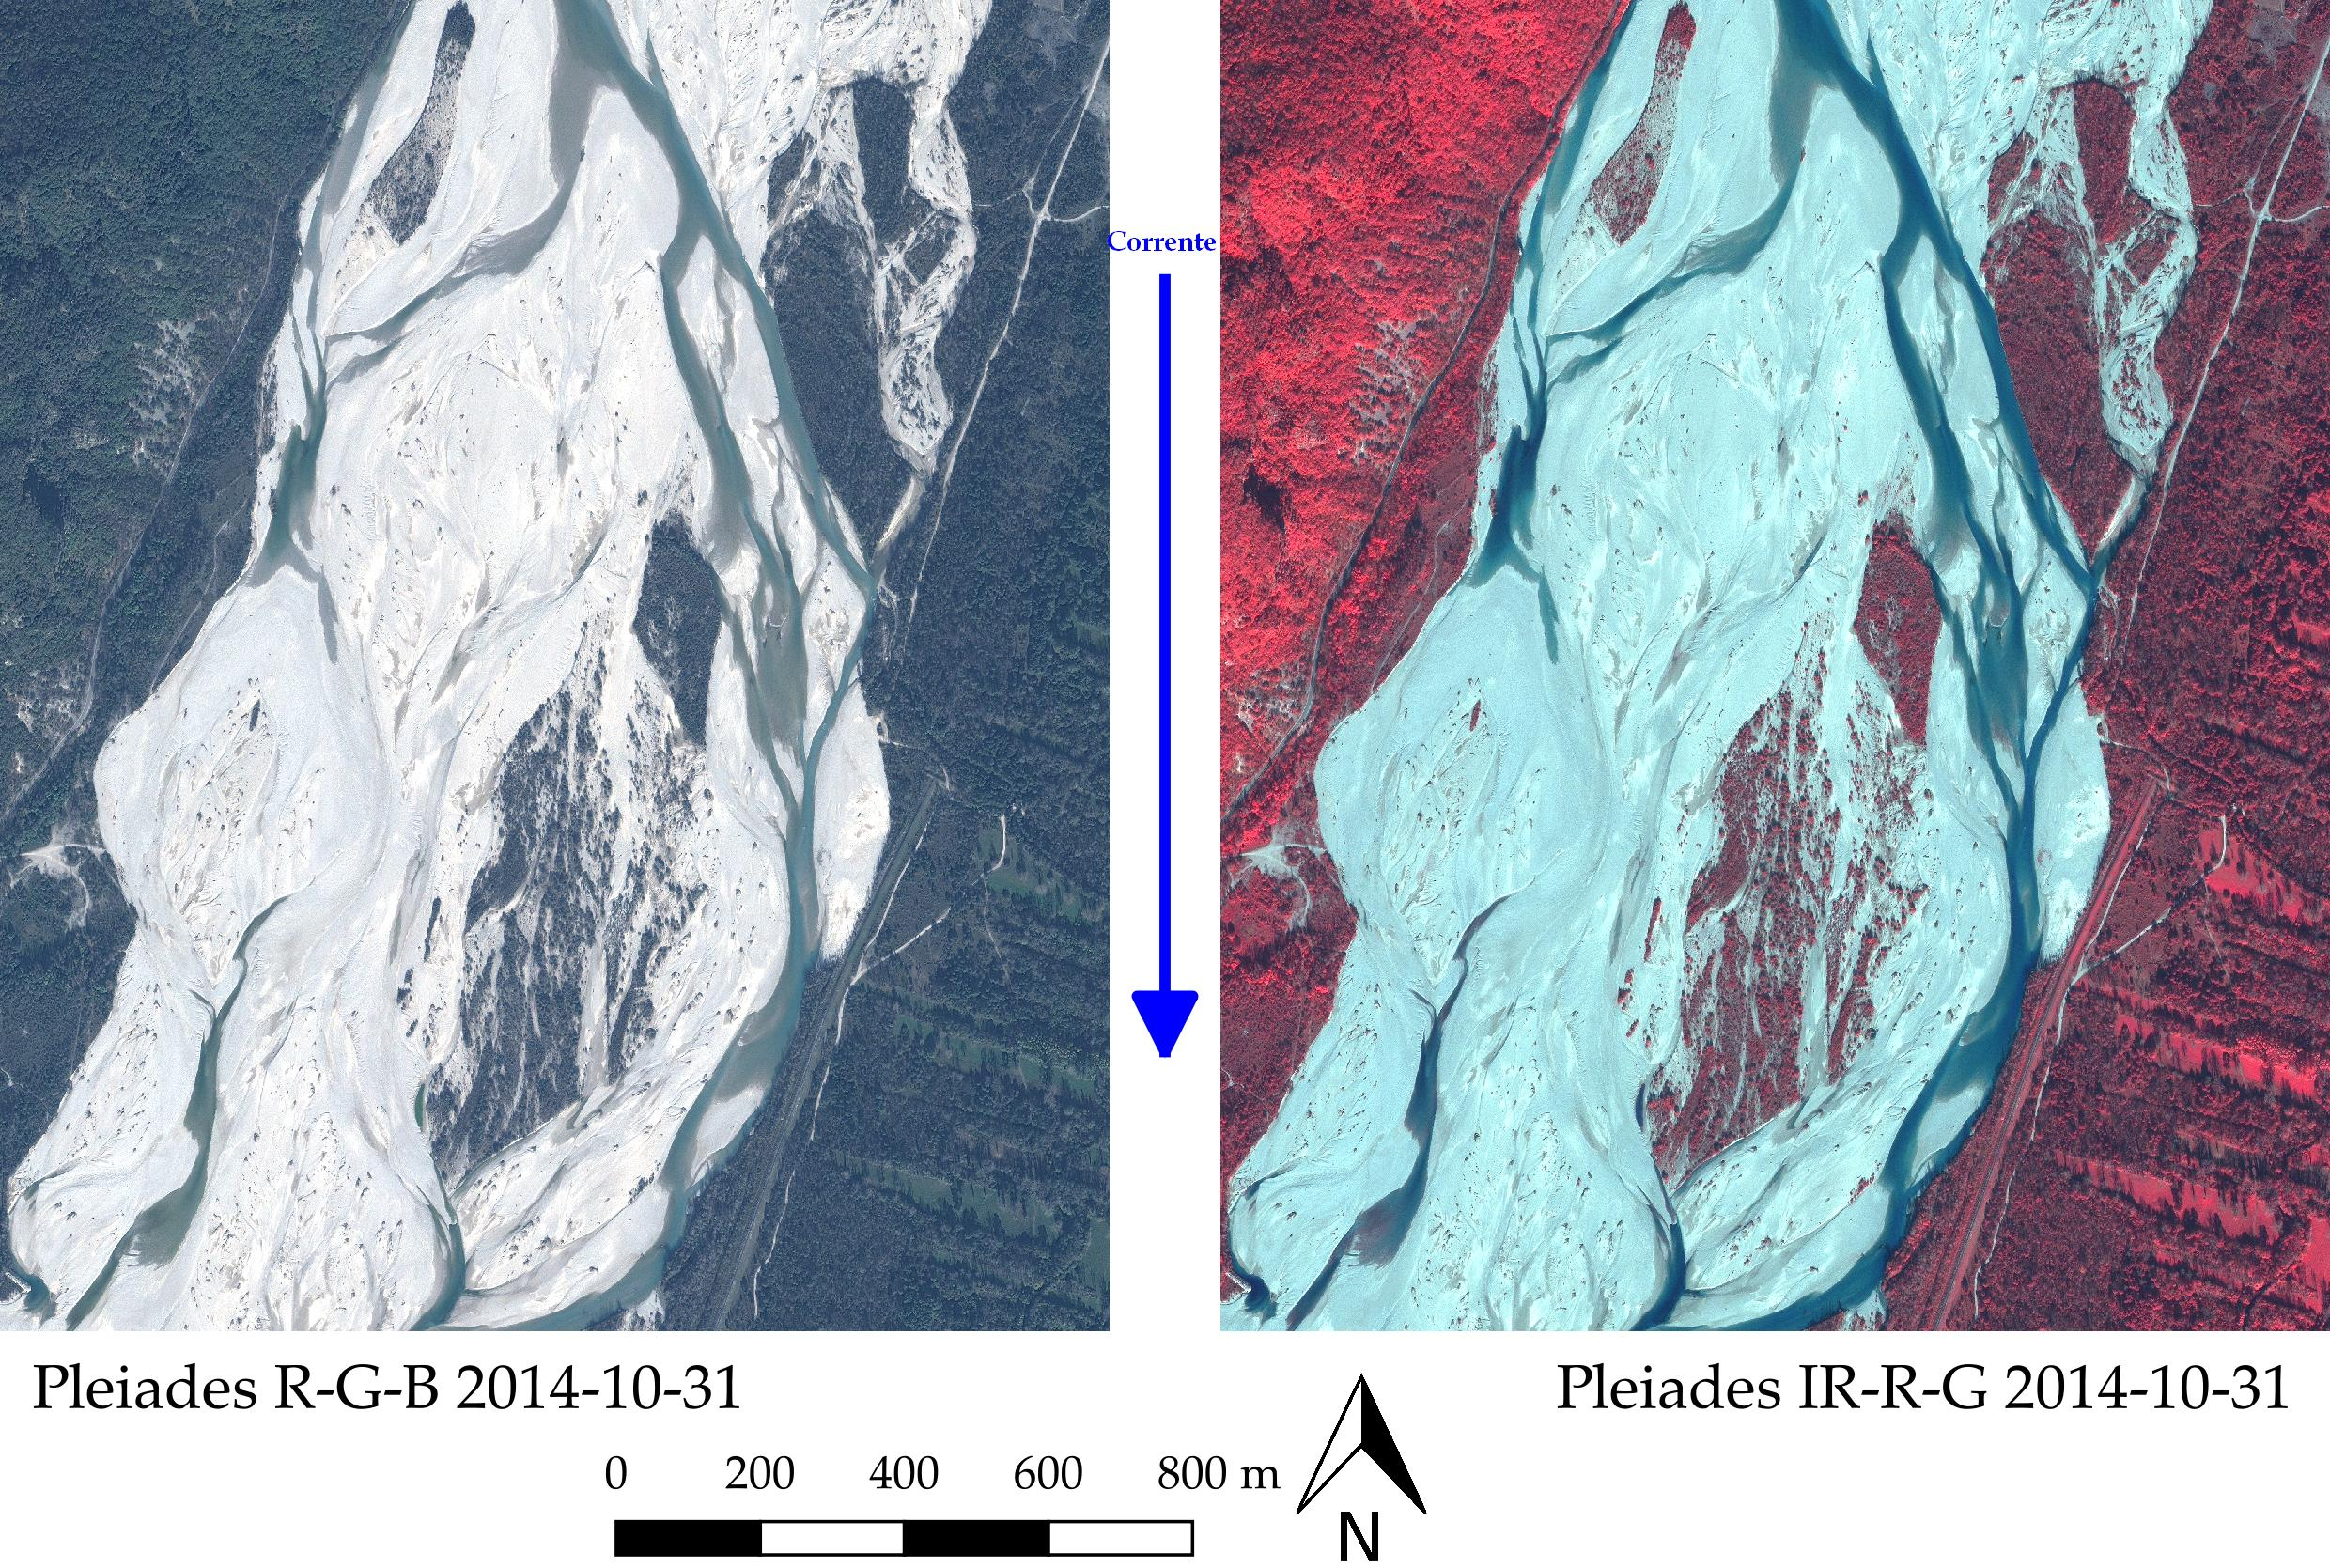
\includegraphics[width=\textwidth]{files/confronto_bande_intro.jpeg}
	\caption[confronto immagini R-G-B e IR-R-G]{confronto di un'immagine in veri colori (R-G-B, a sinistra) con una in falsi colori (IR-R-G, a destra); quest'ultima evidenza la presenza di vegetazione viva rispetto alla ghiaia in alveo e all'acqua nei canali.}
	\label{fig:confronto-bande-intro}
\end{figure}
%
\\
Questo procedimento serve per distinguere più facilmente alcuni elementi e oggetti presenti nelle immagini; per esempio la vegetazione viva riflette particolarmente la banda dell'Infrarosso più vicina al Rosso.



\section{Materiali}
\subsection{Immagini satellitari e rilievi aerei}
Nelle immagini satellitari multibande sia acquisite che di proprietà dell'Università degli Studi di Trento sono state considerate le bande del \emph{Near-InfraRed}~(NIR) e del \emph{Red}~(R), in quanto permettono di distinguere la vegetazione dalle altre coperture del suolo;
le immagini provengono dalle seguenti missioni:
%
\begin{itemize}
	\item satellite Terra, sensore \AST{} Livello~1T (ottenuti in data~21~luglio~2018 e~30~settembre~2018 \squarecite{data:ASTER});  
		\\
		NIR (Banda~3N)~\SIrange[range-phrase={-}]{0.78}{0.86}{\nano\m}, R (Banda~2)~\SIrange[range-phrase={-}]{0.63}{0.69}{\micro\m};
	\item costellazione \Pl{} (\href{https://pleiades.cnes.fr/en/PLEIADES/index.htm}{Centre National d'Etudes Spatiales}\footnote{\texttt{https://pleiades.cnes.fr/en/PLEIADES/index.htm}}), immagini acquistate dall'Università degli Studi di Trento; 
		\\
		NIR~\SIrange[range-phrase={-}]{0.74}{0.94}{\micro\m}, R~\SIrange[range-phrase={-}]{0.59}{0.71}{\micro\m};
	\item satellite \Se{}A-B, sensore~MSI Livello~1C (ottenuti in data 21~luglio 2018 e~21~novembre~2018 tramite il \href{http://scihub.copernicus.eu/}{Copernicus Open Access Hub}\footnote{\texttt{http://scihub.copernicus.eu/}});
		\\
		NIR (Banda~8)~\SIrange[range-phrase={-}]{0.763}{0.908}{\micro\m}, R (Banda~4)~\SIrange[range-phrase={-}]{0.645}{0.683}{\micro\m};
	\item satellite \WV{} (\href{satimagingcorp.s3.amazonaws.com/site/pdf/WV1\_{}WV2\_{}SpectralResponse.pdf}{DigitalGlobe}\footnote{\texttt{satimagingcorp.s3.amazonaws.com/site/pdf/WV1\_{}WV2\_{}SpectralResponse.pdf}}), immagini acquistate dall'Università degli Studi di Trento;
		\\
		NIR (Banda~MS1)~\SIrange[range-phrase={-}]{0.770}{0.895}{\micro\m}, R (Banda~MS2)~\SIrange[range-phrase={-}]{0.630}{0.690}{\micro\m}.
\end{itemize}
%
Le immagini sono state selezionate secondo i seguenti criteri:
%
\begin{itemize}
	\item minima copertura nuvolosa del tratto di studio;
	\item data compresa tra metà aprile e fine ottobre, che è il periodo vegetativo delle piante decidue (\emph{Salix spp.}, \emph{Populus nigra}) che caratterizzano le isole fluviali e la piana alluvionale;
	\item basso livello dell'acqua, per evitare che alcune isole siano sommerse e non visibili;
	\item estensione di almeno qualche decina di chilometri sul tratto di studio.
\end{itemize}
%
Tutte le immagini mostrano la radianza registrata al sensore, sono geometricamente corrette tramite modelli digitali del terreno e georeferenziate secondo la proiezione UTM~33N.

Le ortofoto dell'estate~2011 provengono dal \href{http://www.pcn.minambiente.it/mattm/}{Portale Cartografico Nazionale del Ministero dell'Ambiente e della tutela del territorio e del mare}\footnote{\texttt{http://www.pcn.minambiente.it/mattm/}};
le ortofoto del~2013 sono state ottenute da volo \href{http://www.cgrspa.com/}{CGR}\footnote{\texttt{http://www.cgrspa.com/}} su commissione; 
le ortofoto del~2017 sono state ottenute da \href{https://www.google.com/earth/}{Google Earth}\footnote{\texttt{https://www.google.com/earth/}} (Map data: Google, Digital Globe, European Space Imaging).

Nei mesi di Maggio~2005, Agosto~2010 ed Ottobre~2013 (congiuntamente all'ortofoto) è stato effettuato un rilievo aereo LiDAR, grazie al quale sono a disposizione un DEM (\emph{Digital Elevation Model}) e un CHM (\emph{Canopy Height Model}) per ogni anno: il primo consiste di una mappa con le quote del suolo; il secondo è una mappa di altezza della vegetazione.
Per questi rilievi si ringraziano rispettivamente il UK Natural Environment Research Council, Nicola Surian dell'Università di Padova (progetto CARIPARO) e Yasuhiro Takemon dell'Università di Kyoto.

Il DEM del~2009 proviene dal \href{http://irdat.regione.fvg.it/CTRN/ricerca-cartografia/}{Portale Cartografico della regione autonoma Friuli Venezia Giulia}\footnote{\texttt{http://irdat.regione.fvg.it/CTRN/ricerca-cartografia/}}.

È bene evidenziare che le mappe non hanno tutte la medesima estensione e una piccola parte non comprende tutto il tratto oggetto di studio.
Ciò limita minimamente le analisi che è possibile fare.
\\
Avendo a disposizione 25 immagini per un periodo di studio di quasi \SI{19}{\anni},  si ritiene che la risoluzione temporale sia sufficiente per interpretare i processi che hanno luogo nel Tagliamento: la distanza temporale media tra le mappe è di \SI{274}{\giorni} (circa \SI{0.75}{\anni}), quella minima di \SI{25}{\giorni} e quella massima di \SI{480}{\giorni}.
\\
La risoluzione spaziale varia da~\SIrange[range-phrase={ a }]{15}{0.5}{\m}, adeguata per poter distinguere correttamente le caratteristiche del fiume (limite dell'alveo attivo, isole, canali nella \emph{floodplain}, canali attivi, \ldots).
\\
La \cref{tab:date-orto-sat} mostra le date, la dimensione delle celle delle immagini utilizzate nell'analisi e i tratti validi per ogni immagine.
%%%
\begin{table}[p]
	\centering
	\begin{tabular}{c c S[table-format=2.2] S[range-phrase={$\div$}, list-separator={, }, list-final-separator={, }]}
		\toprule
		Data		&	Tipo		&	\multicolumn{1}{c}{Dim. delle celle \si{[\m]}}	&	\multicolumn{1}{c}{Tratti validi}\\
		\midrule	
		2000-09-17		&	\AST{}		&	15	&	\numrange{1}{21}	\\
		2001-06-07		&	\AST{}		&	15	&	\multicolumn{1}{c}{\numrange[range-phrase={$\div$}]{3}{8}, \numrange[range-phrase={$\div$}]{21}{23}}	\\
		2002-05-18		&	\AST{}		&	15	&	\multicolumn{1}{c}{\numrange[range-phrase={$\div$}]{1}{2}, \numrange[range-phrase={$\div$}]{6}{14}}	\\
		2002-06-12		&	\AST{}		&	15	&	\numrange{14}{23}	\\
		2003-06-22		&	\AST{}		&	15	&	\multicolumn{1}{c}{\numrange[range-phrase={$\div$}]{1}{10}, \numrange[range-phrase={$\div$}]{13}{23}}	\\
		2004-10-14		&	\AST{}		&	15	&	\numrange{2}{23}	\\
		2005-05			&	Rilievo aereo LiDAR	&	2	&	\numrange{6}{14}	\\
		2005-08-30		&	\AST{}		&	15	&	\numrange{1}{23}	\\
		2006-07-16		&	\AST{}		&	15	&	\multicolumn{1}{c}{\numrange[range-phrase={$\div$}]{1}{20}, \numrange[range-phrase={$\div$}]{22}{23}}	\\
		2007-09-21		&	\AST{}		&	15	&	\numrange{1}{23}	\\
		2008-07-05		&	\AST{}		&	15	&	\numrange{1}{23}	\\
		2009			&	DEM			&	20	&	\numrange{1}{23}	\\
		2009-07-08		&	\AST{}		&	15	&	\numrange{3}{23}	\\
		2010-08			&	Rilievo aereo LiDAR	&	1	&	\numlist{7;8;11}	\\
		2010-09-29		&	\AST{}		&	15	&	\numrange{1}{23}	\\
		2011-06-26/07-02	&	Ortofoto	&	1	&	\numrange{6}{12}	\\
		2011-10-02		&	\AST{}		&	15	&	\numrange{1}{23}	\\
		2012-08-01		&	\AST{}		&	15	&	\numrange{1}{23}	\\
		2013-09-05		&	\AST{}		&	15	&	\numrange{1}{23}	\\
		2013-10-22		&	Ortofoto	&	0.2	&	\numlist{7;8;11;12}	\\
		2013-10-22		&	Rilievo aereo LiDAR	&	1	&	\numlist{7;8;11;12}	\\
		2014-09-08		&	\AST{}		&	15	&	\numrange{1}{23}	\\
		2014-10-31		&	\Pl{}	&	0.5	&	\numrange{6}{14}	\\
		2015-08-13		&	\Pl{}	&	0.5	&	\numrange{6}{14}	\\
		2015-09-12		&	\Se{}	&	10	&	\numrange{1}{23}	\\
		2015-10-22		&	\Se{}	&	10	&	\numrange{1}{23}	\\
		2016-09-13		&	\Se{}	&	10	&	\numrange{1}{23}	\\
		2017-04-21		&	\Se{}	&	10	&	\numrange{1}{23}	\\
		2017-06-13		&	\Se{}	&	10	&	\numrange{1}{23}	\\
		2017-06-26/08-02	&	G-Earth	&	0.45	&	\numrange{6}{15}	\\
		2018-06-15		&	\WV{}	&	0.5	&	\numrange{7}{14}	\\
		2018-09-16		&	\Se{}	&	10	&	\numrange{1}{23}	\\
		\bottomrule
	\end{tabular}
	\caption[dettagli delle immagini e rilievi aerei utilizzati]{data e dimensione delle celle delle immagini satellitari, delle ortofoto, del DEM e dei rilievi aerei LiDAR utilizzati.}
	\label{tab:date-orto-sat}
\end{table}


\subsection{Dati idrometrici}
I dati idrometrici orari o semi-orari dal 2000-01-01 al 2018-12-21 presso l'idrometro di Villuzza~(UD) (\SI{46.181}{\degree}N, \SI{12.958}{\degree}E, quota~\SI{240}{\m}~s.l.m.m., corrispondente al ponte di Pinzano) sono stati forniti dalla \href{http://www.protezionecivile.fvg.it/it/rete-idrometeorologica}{rete idrometeorologica della Protezione Civile della Regione Autonoma Friuli Venezia Giulia}\footnote{\texttt{http://www.protezionecivile.fvg.it/it/rete-idrometeorologica}}.
Questi dati riportano l'altezza del pelo libero dell'acqua rispetto ad un livello di riferimento locale dell'idrometro.
La dinamica della morfologia del fondo del fiume non permette di ottenere una scala di deflusso (delle portate) generalmente valida; ciò comunque non costituisce un limite poiché questi dati forniscono adeguate e sufficienti informazioni sulle piene di intensità medio-elevata.
Il grafico in \cref{graph:livelli-matrix} mostra i livelli idrometrici mediati giornalmente; da questi si vede bene come le piene siano generalmente imprevedibili, come abbiano luogo generalmente nei periodi primaverili e autunnali e come si possano alternare anni caratterizzati da pochi eventi con anni che presentano molte piene importanti; si rammenta come proprio questa naturale variabilità del regime delle piene regoli l'abbondanza e la distribuzione delle specie che vivono in ambiente ripario \squarecite{Poff:1997}.
%
\begin{figure}
	\centering
	\tikzsetnextfilename{livelli_matrix}
\begin{tikzpicture}
	\begin{axis}[
		width = \textwidth,
		height = \textwidth,
		enlargelimits = 0,
		ytick distance = 1,
		xtick = {1,31,59,90,120,151,181,212,243,273,304,334,365},
		xticklabels = {{Gennaio}, {Febbraio}, {Marzo},  {Aprile}, {Maggio}, {Giugno}, {Luglio}, {Agosto}, {Settembre}, {Ottobre}, {Novembre}, {Dicembre}},
		xticklabel style = {
			rotate = 90,
		},		
		x tick label as interval,		
		colormap/jet,
		colorbar horizontal,
		colorbar style = {
			xlabel = {Media giornaliera del livello idrometrico},
			x unit = m,
		},	
		]
		\addplot[
			matrix plot*,
			mesh/cols = 365,
			shader = flat corner,
			] % ai dati è stato eliminato il 29 febbraio...! Qualcuno se ne accorgerà mai...?
        	table [x = data, y = anno, point meta = \thisrow{media-gg}] {graphics/data/Dati_Villuzza_matrix.csv};
    \end{axis}
\end{tikzpicture}
	\caption[livelli idrometrici medi giornalieri]{livelli idrometrici medi giornalieri; risulta evidente l'imprevedibilità degli eventi di piena, sebbene questi siano concentrati durante la primavera e l'autunno.}
	\label{graph:livelli-matrix}
\end{figure}

I grafici in \cref{graph:livelli-orto-sat} mostrano rispettivamente i livelli idrometrici e le date di cui si dispongono ortofoto e immagini satellitari (\AST{}, \Pl{}, \Se{}, Google~Earth, \WV{}). 
Nel secondo grafico sono riportati solamente i livelli maggiori di~\SI{1.5}{\m} per mostrare sia le piene di media intensità che quelle più elevate.
Dalla soglia di \SI{2}{\m} si assiste ad una completa connessione di pozze, canali e sorgenti tramite l'inondazione delle barre in ghiaia più alte, iniziando quindi ad esercitare effetti di disturbo sulla vegetazione \squarecite{Bertoldi:2009-2m}.
%
\begin{figure}
	\centering
	\begin{tikzpicture}
	%\begin{groupplot}
	\begin{axis}[
		%name = orto-sat,
		axis y line* = right,
		axis x line* = top,
		%height = .3\textwidth,
		width = \textwidth,
		date coordinates in = x,
		%symbolic y coords = {ASTER,PLEIADES,SENTINEL2,G-EARTH},
		xticklabel = {\year-\month-\day},
		xtick = data,
		ytick = data,
		xticklabel style = {
			rotate = 90,
			anchor = near xticklabel
		},
		enlarge x limits = 0.05,
		enlarge y limits = 0.01,
		ylabel = {Fonte},
		ymax = 3.6,
		ymin = -0.1,
		grid = none,
		only marks,
		]
		\addplot table [x=data, y=numero] {graphics/data/data-orto-sat.txt};
	\end{axis}
	%
	\begin{axis}[
		%name = stages,
		%at = {($(orto-sat.south)-(0,2cm)$)},
		%anchor = north,
		axis y line* = left,
		width = \textwidth,
		date coordinates in = x,
		xticklabel = {\year-\month-\day},
		xticklabel style = {
			rotate = 45,
			anchor = near xticklabel
		},
		enlarge x limits = 0.05,
		enlarge y limits = 0.01,
		ymax = 3.6,
		ymin = -0.1,
		ylabel = {Livello idrometrico},
		grid = major,
		no markers,
		]
		\addplot table [x=data, y=media-gg] {graphics/data/Dati_Villuzza.csv};
	\end{axis}
\end{tikzpicture}
	\tikzsetnextfilename{livelli_2m+imm}
\begin{tikzpicture}
	\begin{axis}[
		width = \textwidth,
		height = 0.5\textwidth,
		date coordinates in = x,
		date ZERO = 2000-01-01,
		xticklabel = {$\year$},
		xticklabel style = {
			rotate = 80,
			anchor = near xticklabel
		},
		xtick distance = 732,
		enlarge x limits = 0.05,
		enlarge y limits = 0.01,
		ymax = 3.7,
		ymin = 1.95,
		ylabel = {Livello idrometrico \si{[\m]}},
		grid = major,
		]
		\addplot+ 
			[red, mark=x, semithick, style=solid, mark=x]
			coordinates {(2000-09-17, 2)(2000-09-17, 3.7)};
		\addplot+ 
			[red, semithick, style=solid, mark=x]
			coordinates {(2001-06-07, 2)(2001-06-07, 3.7)};
		\addplot+
        	[red, semithick, style=solid, mark=x]
        	coordinates {(2002-05-18, 2)(2002-05-18, 3.7)};
		\addplot+
        	[red, semithick, style=solid, mark=x]
        	coordinates {(2002-06-12, 2)(2002-06-12, 3.7)};
		\addplot+
        	[red, semithick, style=solid, mark=x]
        	coordinates {(2003-06-22, 2)(2003-06-22, 3.7)};
		\addplot+
        	[red, semithick, style=solid, mark=x]
        	coordinates {(2004-10-14, 2)(2004-10-14, 3.7)};
		\addplot+
        	[green, semithick, style=solid, mark=x]
        	coordinates {(2005-05-01, 2)(2005-05-01, 3.7)};
		\addplot+
        	[red, semithick, style=solid, mark=x]
        	coordinates {(2005-08-30, 2)(2005-08-30, 3.7)};
		\addplot+
        	[red, semithick, style=solid, mark=x]
        	coordinates {(2006-07-16, 2)(2006-07-16, 3.7)};
		\addplot+
        	[red, semithick, style=solid, mark=x]
        	coordinates {(2007-09-21, 2)(2007-09-21, 3.7)};
		\addplot+
        	[red, semithick, style=solid, mark=x]
        	coordinates {(2008-07-05, 2)(2008-07-05, 3.7)};
		\addplot+
        	[red, semithick, style=solid, mark=x]
        	coordinates {(2009-07-08, 2)(2009-07-08, 3.7)};
		\addplot+
        	[green, semithick, style=solid, mark=x]
        	coordinates {(2010-08-01, 2)(2010-08-01, 3.7)};
		\addplot+
        	[red, semithick, style=solid, mark=x]
        	coordinates {(2010-09-29, 2)(2010-09-29, 3.7)};
		\addplot+
        	[green, semithick, style=solid, mark=x]
        	coordinates {(2011-07-01, 2)(2011-07-01, 3.7)};
		\addplot+
        	[red, semithick, style=solid, mark=x]
        	coordinates {(2012-08-01, 2)(2012-08-01, 3.7)};
		\addplot+
        	[red, semithick, style=solid, mark=x]
        	coordinates {(2013-09-05, 2)(2013-09-05, 3.7)};
		\addplot+
        	[green, semithick, style=solid, mark=x]
        	coordinates {(2013-10-22, 2)(2013-10-22, 3.7)};
		\addplot+
        	[red, semithick, style=solid, mark=x]
        	coordinates {(2014-09-08, 2)(2014-09-08, 3.7)};
		\addplot+
        	[black, semithick, style=solid, mark=x]
        	coordinates {(2014-10-31, 2)(2014-10-31, 3.7)};
       	\addplot+
        	[black, semithick, style=solid, mark=x]
        	coordinates {(2015-08-13, 2)(2015-08-13, 3.7)};
		\addplot+
        	[cyan, semithick, style=solid, mark=x]
        	coordinates {(2015-09-12, 2)(2015-09-12, 3.7)};
		\addplot+
        	[cyan, semithick, style=solid, mark=x]
        	coordinates {(2015-10-22, 2)(2015-10-22, 3.7)};
		\addplot+
        	[cyan, semithick, style=solid, mark=x]
        	coordinates {(2016-09-13, 2)(2016-09-13, 3.7)};
		\addplot+
        	[cyan, semithick, style=solid, mark=x]
        	coordinates {(2017-04-21, 2)(2017-04-21, 3.7)};
		\addplot+
        	[cyan, semithick, style=solid, mark=x]
        	coordinates {(2017-06-13, 2)(2017-06-13, 3.7)};
		\addplot+
        	[green, semithick, style=solid, mark=x]
        	coordinates {(2017-07-07, 2)(2017-07-07, 3.7)};
       	\addplot+
        	[violet, semithick, style=solid, mark=x]
        	coordinates {(2018-06-15, 2)(2018-06-15, 3.7)};
		\addplot+
        	[cyan, semithick, style=solid, mark=x]
        	coordinates {(2018-09-16, 2)(2018-09-16, 3.7)};
		\addplot+
        	[blue, solid, no markers]
        	table [x=data, y=media-gg] {graphics/data/Dati_Villuzza.csv};
	\end{axis}
\end{tikzpicture}
	\caption[livelli idrometrici e foto aeree - satellitari]{in alto il livello idrometrico (in blu) presso l'idrometro di Villuzza, registrato con frequenza oraria o semi-oraria. 
	In basso un ingrandimento per i livelli medi giornalieri superiori a~\SI{1.5}{\m}, che sono indice di piene con effetti non trascurabili.
	I simboli indicano le immagini satellitari e le ortofoto considerate (\AST{} in rosso, ortofoto, rilievi aerei LiDAR e G-Earth in verde, \Pl{} in nero, \Se{} in azzurro, \WV{} in viola).}
	\label{graph:livelli-orto-sat}
\end{figure}



\section{Strumenti}
Per eseguire le analisi sulle immagini aeree e satellitari sono stati utilizzati i GIS GRASS \squarecite{soft:GRASS} e QGIS \squarecite{soft:QGIS}. 
\\
Per l'estrazione delle immagini satellitari \AST{} dagli archivi \texttt{.hdf} è stato usato SCP, plugin di QGIS \squarecite{soft:SCP}. 
\\
Per il download delle ortofoto dell'estate~2017 si è utilizzato \href{https://github.com/sourcepole/qgis-openlayers-plugin}{OpenLayers}\footnote{\texttt{https://github.com/sourcepole/qgis-openlayers-plugin}}, plugin di QGIS.
\\
Per le analisi dei dati sono stati realizzati script in Python~2.7.5 utilizzando la libreria PyGRASS\footnote{\texttt{https://grass.osgeo.org/programming7/}} \squarecite{Zambelli:2013-pygrass} e in Python~3.7.1\footnote{\texttt{https://www.python.org}}.

%----------------------------------------------------------



\chapter{Analisi della vegetazione nelle isole}
\section{Quantità di vegetazione in alveo}
Si è quantificato l'areale delle isole presenti in alveo avendo accortezza di distinguerlo chiaramente dall'areale della \emph{floodplain}, il quale è soggetto a dinamiche diverse rispetto alle isole.

\subsection{Metodi: classificare l'alveo}
Per classificare il terreno occupato dall'alveo è stato seguito l'approccio di altri autori in analisi simili eseguite su immagini \AST{} e LandSat~TM \squarecites{Bertoldi:2011-ASTER}{Henshaw:2013-LandSat}.
%
\begin{description}
	\item[Maschera computazionale] 
	Dapprima è stata individuata manualmente una maschera di calcolo che comprendesse l'alveo attivo e la parte di piana alluvionale che è stata erosa quando coinvolta nelle piene; 
	tale maschera si estende da Tolmezzo al ponte di Madrisio
	(\cref{fig:esempio-maschera}). 
	Applicandola, il dominio computazionale è stato ridotto a comprendere l'inviluppo degli alvei attivi che si sono succeduti dall'immagine del~2000 a quella del~2018.
	%
	\begin{figure}[t]
		\centering
		\begin{subfigure}[b]{0.4\textwidth}
			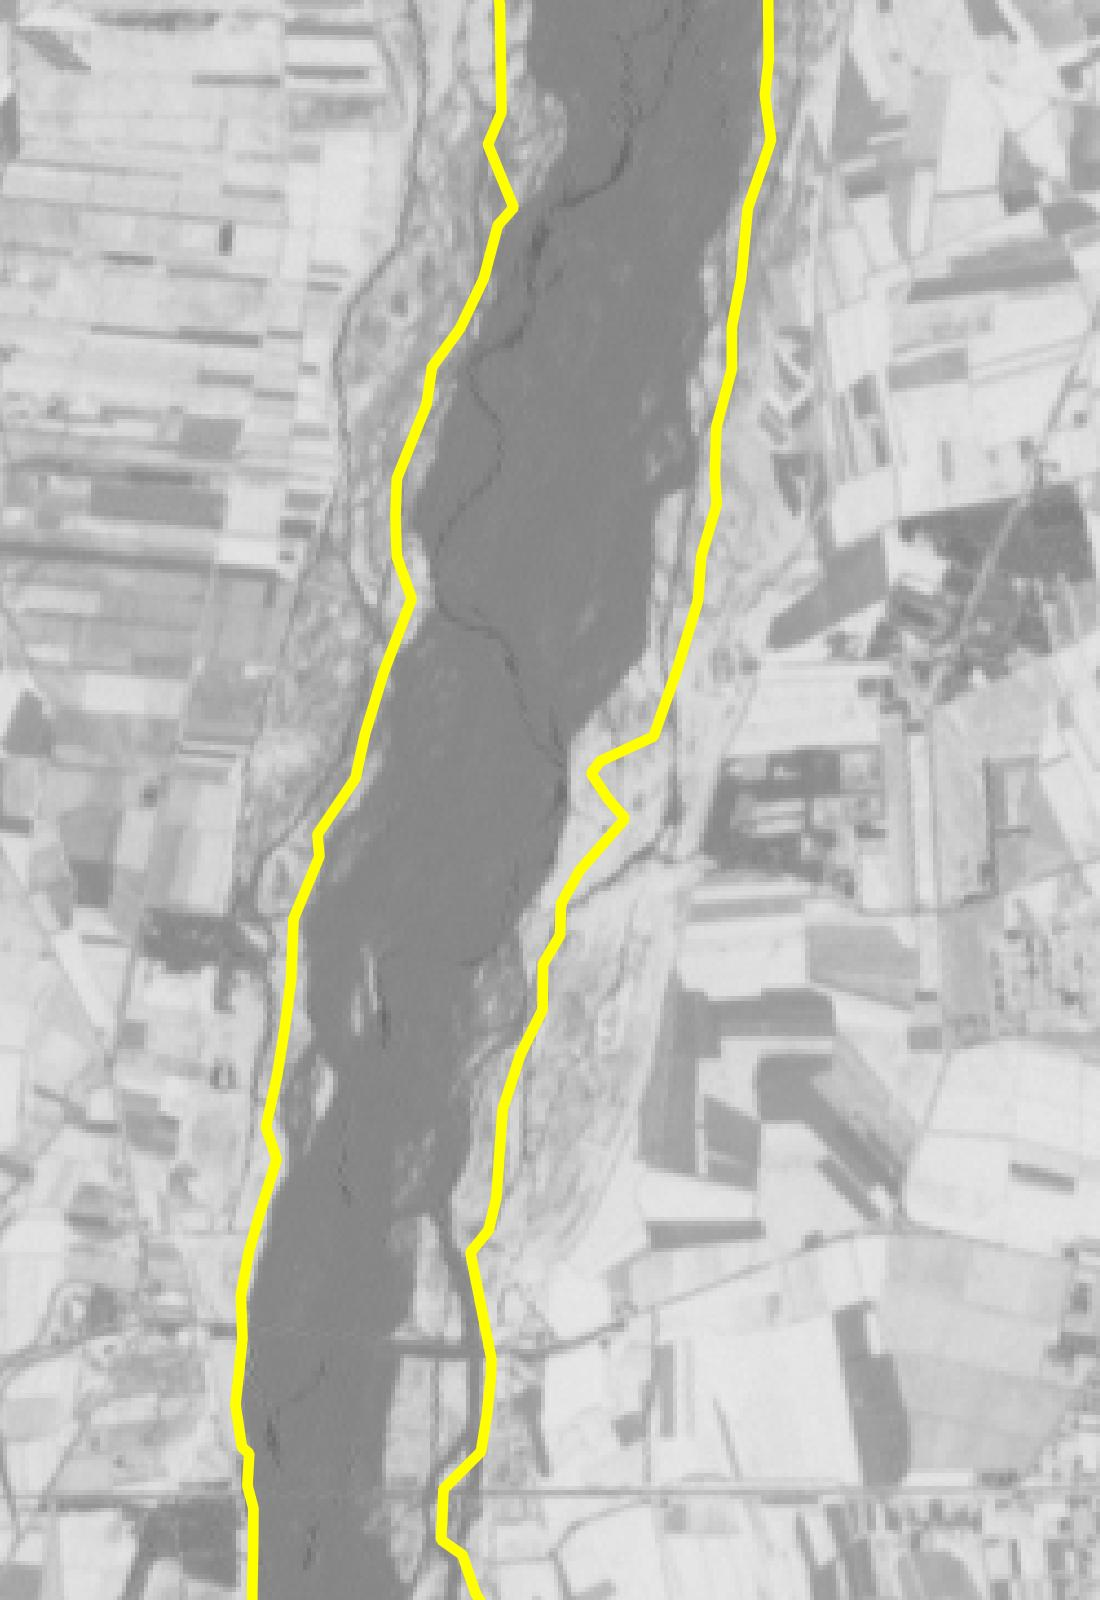
\includegraphics[width=\textwidth]{files/esempio_mask_2002_06_12.jpeg}
			\caption{\AST{} 2002-06-12.}
		\end{subfigure}
		\qquad
		\begin{subfigure}[b]{0.4\textwidth}
			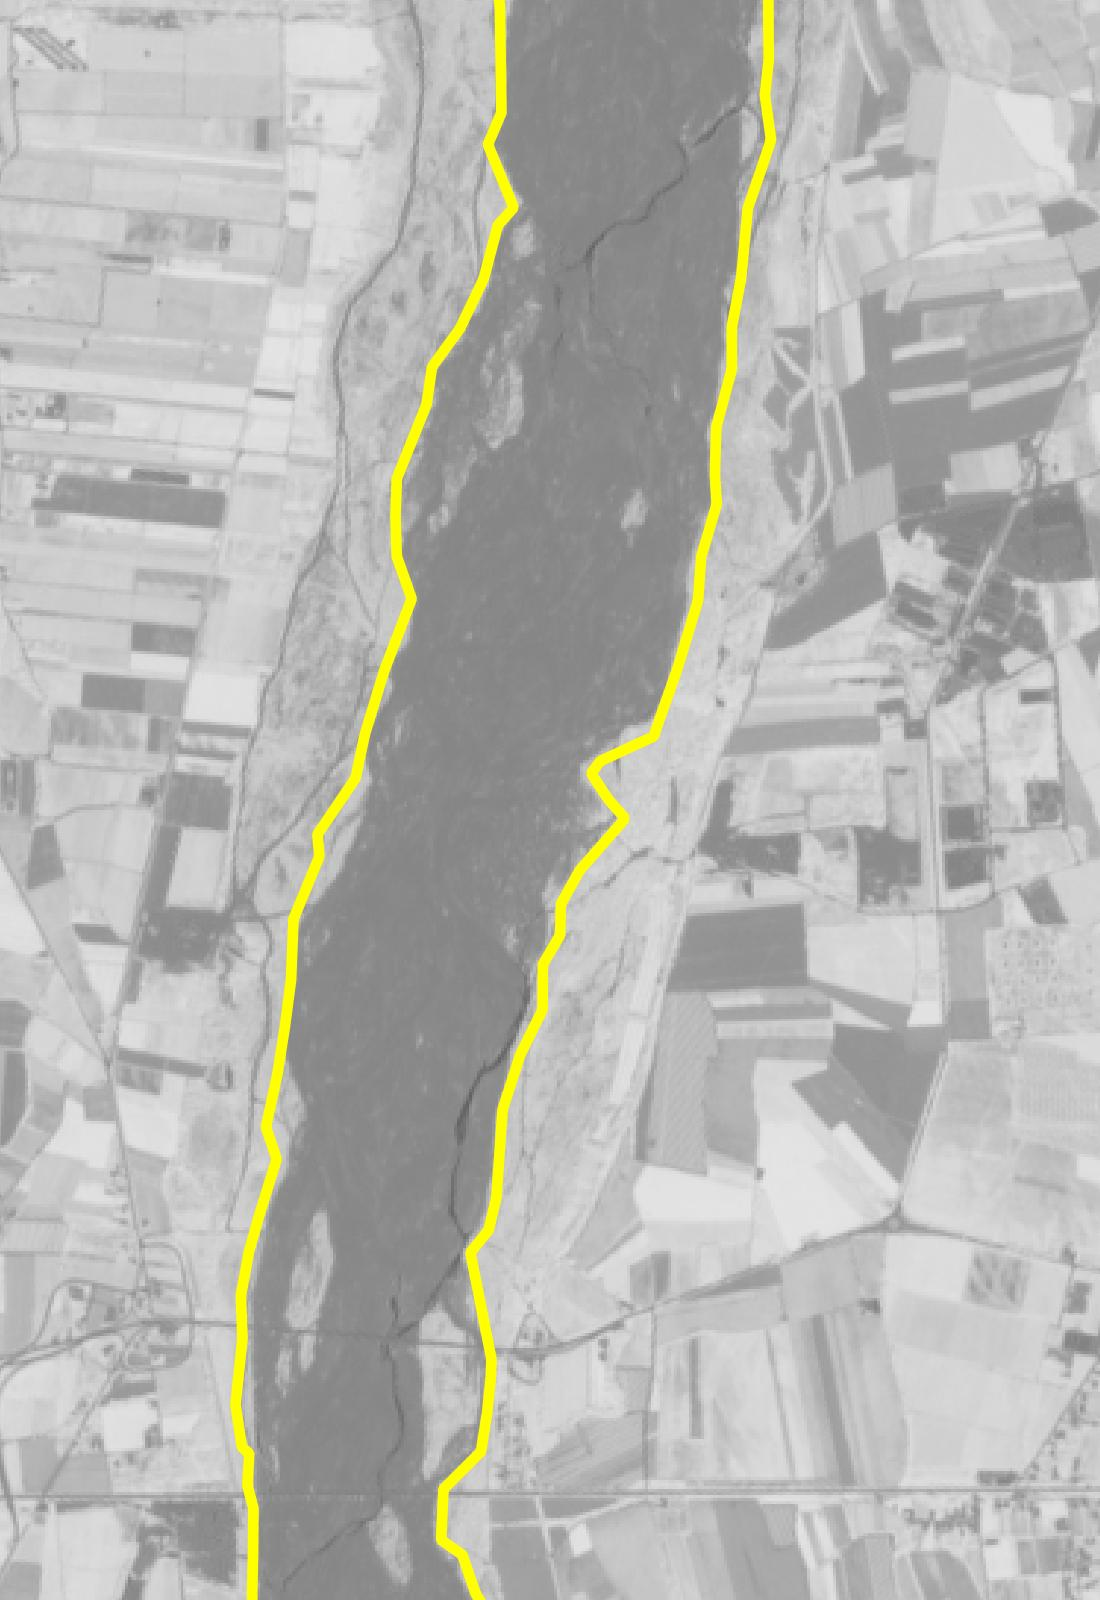
\includegraphics[width=\textwidth]{files/esempio_mask_2015_09_12.jpeg}
			\caption{\Se{} 2015-09-12.}
		\end{subfigure}
		\caption[definizione della maschera per limitare il dominio computazionale]
			{esempio in cui si vede come la maschera utilizzata per limitare il dominio computazionale (in giallo) sia il risultato dell'inviluppo degli alvei attivi che si sono modificati nel tempo; le immagini sono le mappe di NDVI.}
		\label{fig:esempio-maschera}
	\end{figure}
	%
	%
	\item[NDVI] 
	In questa area è stato calcolato il \emph{Normalized Difference Vegetation Index} (NDVI) grazie alle bande del \emph{Near Infrared} (NIR) e del \emph{Red} (R)
	%
	\begin{equation}
		%\notag
		NDVI = \frac{NIR - R}{NIR + R} \quad .
		\label{eq:ndvi}
	\end{equation}
	%
	%
	\item[Aree campione]
	\`{E} stata effettuata una digitalizzazione manuale di alcune aree campione per le immagini \AST{} del~2005-08-30 ($\sim 70$) e del~2012-08-01 ($\sim 100$), le immagini Plaiades del~2014-10-31 ($\sim 40$) e del~2015-06-13 ($\sim 40$), l'immagine \Se{} del~2017-04-21 ($\sim 45$) e l'immagine \WV{} del 2018-06-15 ($\sim 55$) (\cref{fig:esempio-aree-campione}).
	Sono state selezionate immagini per ogni satellite poiché ciascuno è sensibile a bande leggermente diverse. 
	\\
	Queste aree campione sono state suddivise in tre classi: vegetazione, alveo attivo e canale.
	%
	\begin{figure}[ht]
		\centering
		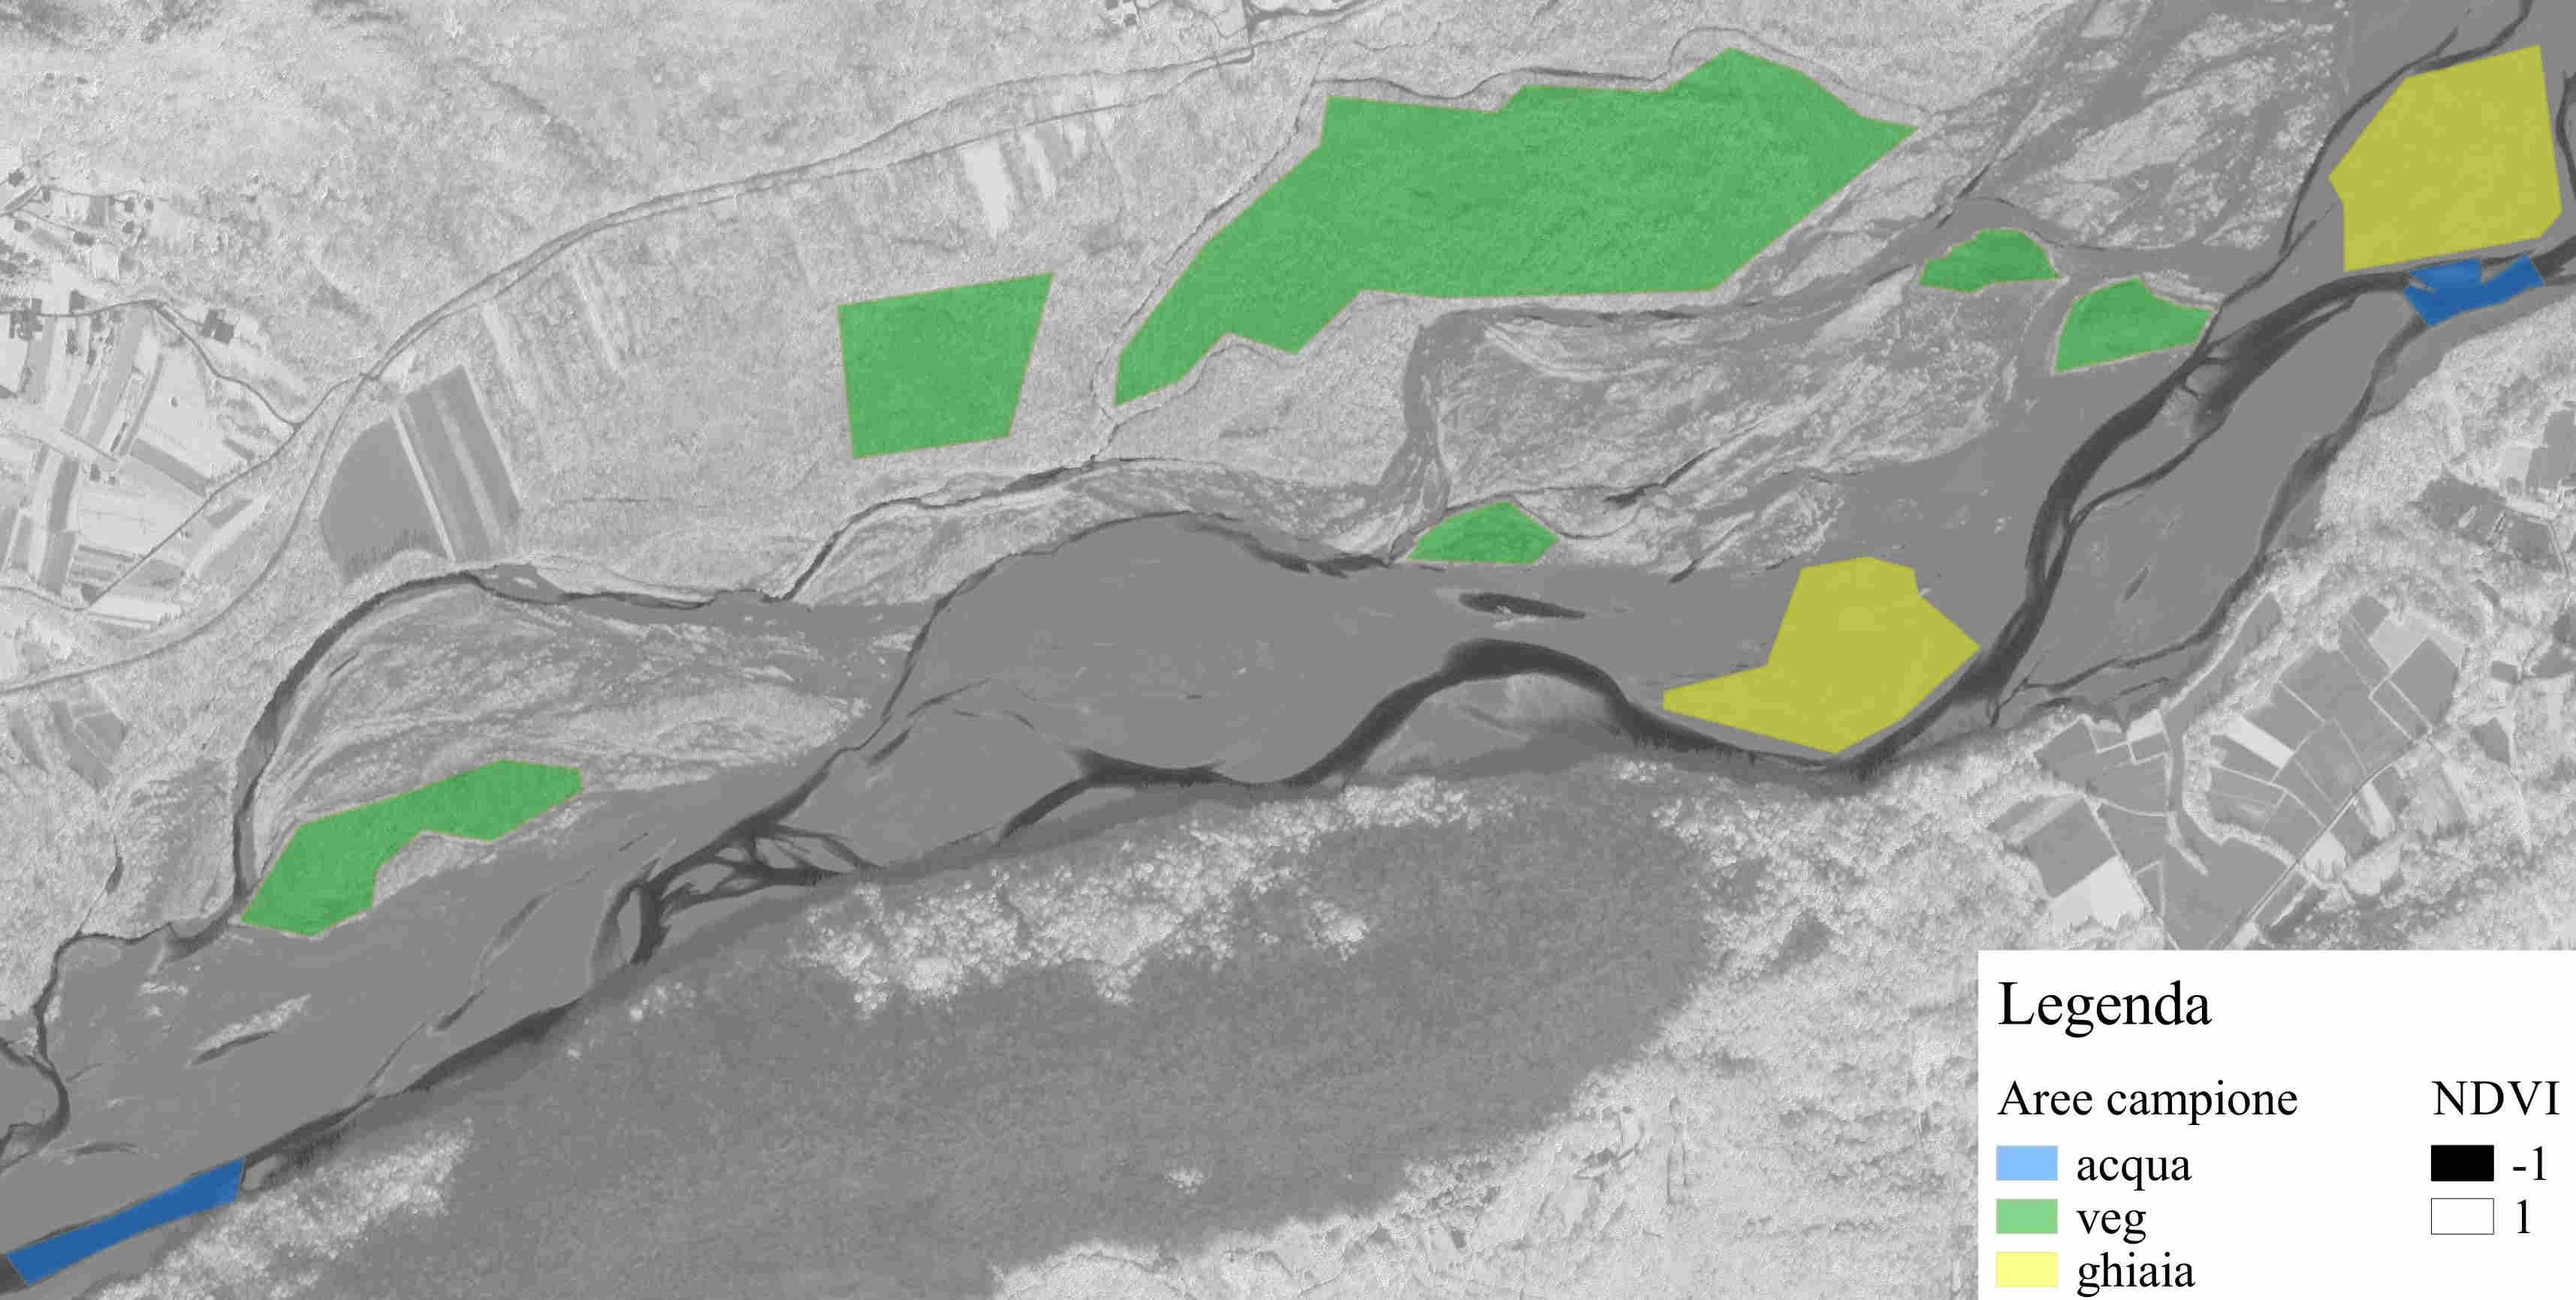
\includegraphics[width=\textwidth]{files/esempio_aree_campione_2014_10_31.jpeg}
		\caption[esempio di aree campione per calcolare la distribuzione dell'NDVI]{esempio di digitalizzazione di alcune aree campione per l'immagine \Pl{} del~2014-10-31; sullo sfondo la mappa dell'NDVI.}
		\label{fig:esempio-aree-campione}
	\end{figure}
	%
	%
	\item[Percentili aree campione]
	Per ogni immagine si è osservata la distribuzione dell'NDVI in ogni classe (\cref{graph:percentili}).
	% 
	\begin{figure}[ht]
		\centering
		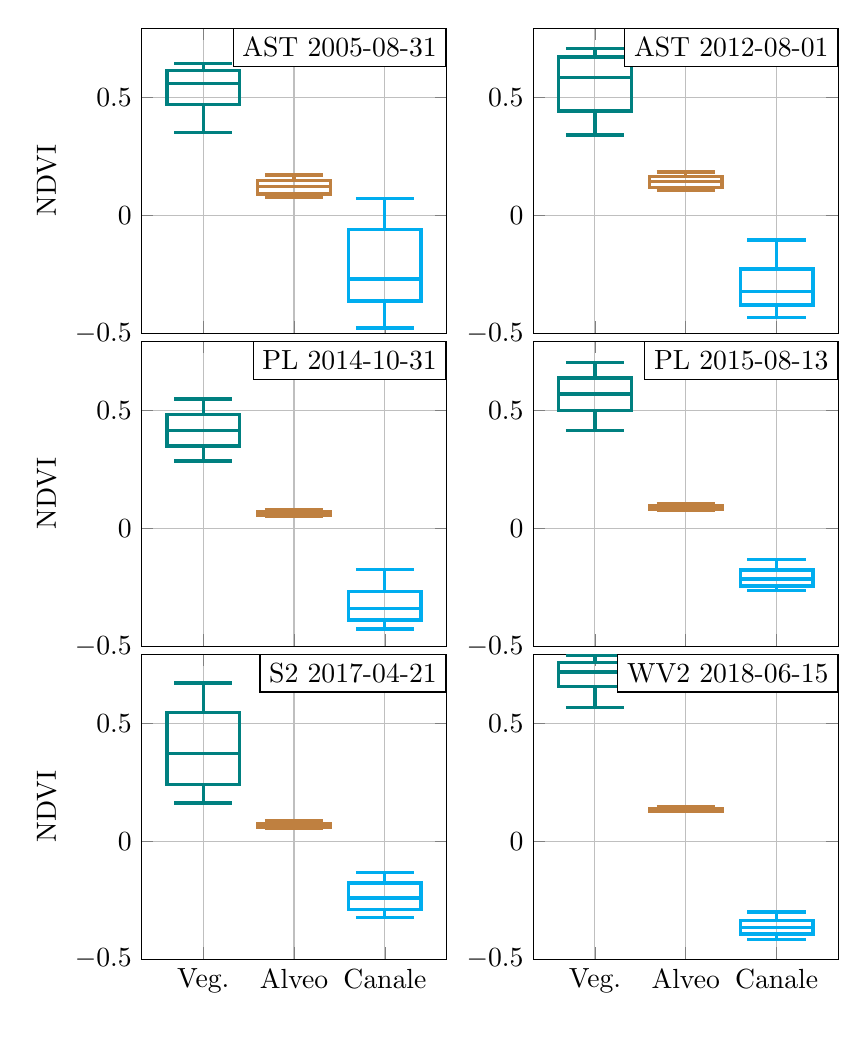
\begin{tikzpicture}
	\begin{groupplot}[
		group style = {
			group size = 2 by 3,
			ylabels at = edge left,
			x descriptions at = edge bottom,
			horizontal sep = 1.1cm,
			vertical sep = 0.1cm,
		},
		width = 0.45\textwidth,
		height = 0.45\textwidth,
		ylabel = NDVI,
		boxplot/draw direction = y,
		xtick = {1,2,3},
		xticklabels = {Veg., Alveo, Canale},
		ymax = 0.795,
		ymin = -0.50,
		grid = major,
	]
	\nextgroupplot % ASTER 2005-08-31
		\addplot+ [ % vegetazione
			teal, very thick,
			boxplot prepared = {
				lower whisker = 0.353656,
				lower quartile = 0.470411,
				median = 0.560063,
				upper quartile = 0.614701,
				upper whisker = 0.644957,
				},
        	]
        	coordinates {};
		\addplot+ [ % alveo attivo
			brown, very thick,
			boxplot prepared = {
				lower whisker = 0.077472,
				lower quartile = 0.091653,
				median = 0.122488,
				upper quartile = 0.149573,
				upper whisker = 0.171459,
				},
        	]
        	coordinates {};
		\addplot+ [ % canale
			cyan, very thick,
			boxplot prepared = {
				lower whisker = -0.477885,
				lower quartile = -0.362798,
				median = -0.269905,
				upper quartile = -0.058787,
				upper whisker = 0.072414,
				},
        	]
        	coordinates {};
        \node [fill = white, draw = black, anchor = north east] 
        	at (axis description cs: 1,1) {AST 2005-08-31};
	%------------------------------------------------------
	\nextgroupplot % ASTER 2012-08-01
		\addplot+ [ % vegetazione
			teal, very thick,
			boxplot prepared = {
				lower whisker = 0.341613,
				lower quartile = 0.444200,
				median = 0.586294,
				upper quartile = 0.672889,
				upper whisker = 0.709027,
				},
        	]
        	coordinates {};
		\addplot+ [ % alveo attivo
			brown, very thick,
			boxplot prepared = {
				lower whisker = 0.10506,
				lower quartile = 0.117969,
				median = 0.143631,
				upper quartile = 0.16549,
				upper whisker = 0.184871,
				},
        	]
        	coordinates {};
		\addplot+ [ % canale
			cyan, very thick,
			boxplot prepared = {
				lower whisker = -0.432201,
				lower quartile = -0.379825,
				median = -0.322239,
				upper quartile = -0.226459,
				upper whisker = -0.103914,
				},
        	]
        	coordinates {};
        \node [fill = white, draw = black, anchor = north east] 
        	at (axis description cs: 1,1) {AST 2012-08-01};
	%------------------------------------------------------
	\nextgroupplot % Pleiades 2014-10-31
		\addplot+ [ % vegetazione
			teal, very thick,
			boxplot prepared = {
				lower whisker = 0.286467,
				lower quartile = 0.350238,
				median = 0.415502,
				upper quartile = 0.483495,
				upper whisker = 0.549505,
				},
        	]
        	coordinates {};
		\addplot+ [ % alveo attivo
			brown, very thick,
			boxplot prepared = {
				lower whisker = 0.049796,
				lower quartile = 0.055794,
				median = 0.063049,
				upper quartile = 0.07173,
				upper whisker = 0.081427,
				},
        	]
        	coordinates {};
		\addplot+ [ % canale
			cyan, very thick,
			boxplot prepared = {
				lower whisker = -0.426415,
				lower quartile = -0.387978,
				median = -0.338308,
				upper quartile = -0.266515,
				upper whisker = -0.175373,
				},
        	]
        	coordinates {};
        \node [fill = white, draw = black, anchor = north east] 
        	at (axis description cs: 1,1) {PL 2014-10-31};
	%------------------------------------------------------
	\nextgroupplot % Pleiades 2015-08-13
		\addplot+ [ % vegetazione
			teal, very thick,
			boxplot prepared = {
				lower whisker = 0.415693,
				lower quartile = 0.5,
				median = 0.570359,
				upper quartile = 0.638507,
				upper whisker = 0.704044		
,
				},
        	]
        	coordinates {};
		\addplot+ [ % alveo attivo
			brown, very thick,
			boxplot prepared = {
				lower whisker = 0.075052,
				lower quartile = 0.080858,
				median = 0.087921,
				upper quartile = 0.096031,
				upper whisker = 0.106198,
				},
        	]
        	coordinates {};
		\addplot+ [ % canale
			cyan, very thick,
			boxplot prepared = {
				lower whisker = -0.262599,
				lower quartile = -0.244228,
				median = -0.214393,
				upper quartile = -0.176471,
				upper whisker = -0.132762,
				},
        	]
        	coordinates {};
        \node [fill = white, draw = black, anchor = north east] 
        	at (axis description cs: 1,1) {PL 2015-08-13};
	%------------------------------------------------------
	\nextgroupplot % Sentinel2 2017-04-21
		\addplot+ [ % vegetazione
			teal, very thick,
			boxplot prepared = {
				lower whisker = 0.163722,
				lower quartile = 0.241916,
				median = 0.374344,
				upper quartile = 0.548241,
				upper whisker = 0.672782,
				},
        	]
        	coordinates {};
		\addplot+ [ % alveo attivo
			brown, very thick,
			boxplot prepared = {
				lower whisker = 0.056176,
				lower quartile = 0.061278,
				median = 0.067681,
				upper quartile = 0.076396,
				upper whisker = 0.089304,
				},
        	]
        	coordinates {};
		\addplot+ [ % canale
			cyan, very thick,
			boxplot prepared = {
				lower whisker = -0.322237,
				lower quartile = -0.288822,
				median = -0.239533,
				upper quartile = -0.177094,
				upper whisker = -0.131119,
				},
        	]
        	coordinates {};
        \node [fill = white, draw = black, anchor = north east] 
        	at (axis description cs: 1,1) {S2 2017-04-21};
	%------------------------------------------------------
	\nextgroupplot % WorldView2 2018-06-15
		\addplot+ [ % vegetazione
			teal, very thick,
			boxplot prepared = {
				lower whisker = 0.569665,
				lower quartile = 0.657917,
				median = 0.719523,
				upper quartile = 0.759148,
				upper whisker = 0.791594,
				},
        	]
        	coordinates {};
		\addplot+ [ % alveo attivo
			brown, very thick,
			boxplot prepared = {
				lower whisker = 0.126214,
				lower quartile = 0.129661,
				median = 0.13373,
				upper quartile = 0.138542,
				upper whisker = 0.149326,
				},
        	]
        	coordinates {};
		\addplot+ [ % canale
			cyan, very thick,
			boxplot prepared = {
				lower whisker = -0.416974,
				lower quartile = -0.392405,
				median = -0.365385,
				upper quartile = -0.335135,
				upper whisker = -0.29979,
				},
        	]
        	coordinates {};
        \node [fill = white, draw = black, anchor = north east] 
        	at (axis description cs: 1,1) {WV2 2018-06-15};
	\end{groupplot}
\end{tikzpicture}

		\caption[\emph{boxplot} dell'NDVI nelle aree campione in quattro immagini satellitari]{\emph{boxplot} dell'NDVI nelle aree campione in quattro immagini satellitari; i baffi indicano il 10mo e il 90mo percentile, gli estremi della scatola rappresentano il 25mo e il 75mo percentile, la linea nella scatola è la mediana.}
		\label{graph:percentili}
	\end{figure}
	%
	%
	\item[Soglie NDVI] 
	Da tali grafici sono state ottenute delle soglie di NDVI per classificare le immagini satellitari (\cref{tab:ndvi-soglia}); per l'immagine \WV{} la soglia che distingue vegetazione da alveo attivo è maggiore. 
	Le soglie sono leggermente maggiori a quanto riportato in letteratura \squarecites{Bertoldi:2011-ASTER}{Henshaw:2013-LandSat} poiché in questo modo c'è una maggior corrispondenza con i dati utilizzati per validare il processo (riportati di seguito).
	%
	\begin{table}[ht]
		\centering
		\begin{tabular}{
			c 
			S[table-format=1.2]@{\,}
			c@{\,}
			c@{\,}
			c@{\,}
			S[table-format=1.2]
			S[table-format=1.1]@{\,}
			c@{\,}
			c@{\,}
			c@{\,}
			S[table-format=1.1]
			}
			\toprule
			&	\multicolumn{5}{c}{\textbf{Soglie AST PL S2}}	&	\multicolumn{5}{c}{\textbf{Soglie WV2}}	\\
			\midrule
			Vegetazione		&	0.25	&	$\leq$	&	NDVI	&			&		& 	0.3	&	$\leq$	&	NDVI	&			& 	\\
			Alveo attivo	&	0.0	&	$\leq$	&	NDVI	&	$<$		&	0.25	&	0.0	&	$\leq$	&	NDVI	&	$<$		&	0.3\\
			Canale			&		&			&	NDVI	&	$<$		&	0.0	&		&			&	NDVI	&	$<$		&	0.0\\
			\bottomrule
		\end{tabular}
		\caption[soglie NDVI]{soglie di NDVI per la classificazione delle immagini satellitari.}
		\label{tab:ndvi-soglia}
	\end{table}
	%
	%
	\item[Isole e \emph{Floodplain}]
	Tramite una procedura semi-automatica e con il supporto di Google Earth, la classe della vegetazione è stata suddivisa in \emph{floodplain} e isole. 
	Tale procedura si basa sul fatto che la maschera computazionale comprende parte della piana alluvionale e che le isole sono completamente circondate dalla ghiaia dell'alveo durante periodi di magra.
	\\
	Successivamente, un controllo visivo del risultato e una correzione manuale di alcune celle hanno permesso sia di distinguere correttamente le isole, sia di evitare che isole molto prossime alla \emph{floodplain} ne fossero considerate parte; la classe delle celle corrette è stata aggiunta alla classificazione.
	%
	%
	\item[Nuvole e nodata] Alcune immagini presentano una lieve copertura nuvolosa che si estende nella maschera; queste zone sono state manualmente delimitate poiché presentano valori NDVI alterati.
	\\
	Altre immagini hanno un'estensione limitata rispetto alla maschera; questo porta ad avere aree prive di dati (\texttt{nodata}).
	\\
	Alla classificazione sono state aggiunte la classe delle nuvole e dei \texttt{nodata}.
	%
	%
	\item[Classificazione finale dei tratti] La \cref{tab:class_tratti} mostra le classi in cui è stato classificato ognuno dei 23~tratti; la \cref{fig:class_is_fl} ne mostra un esempio.
	%
	\begin{table}[ht]
		\centering
		\begin{tabular}{
			c 
			c
			}
			\toprule
			\textbf{Macroclasse}	&	\textbf{Classe}	\\
			\midrule
			Vegetazione		&	Isola	\\
							&	Floodplain	\\
			Alveo attivo	&	Cella corretta	\\
							&	Ghiaia	\\
							&	Canale	\\
			Altro			&	Nuvola	\\
							&	Nodata	\\
			\bottomrule
		\end{tabular}
		\caption[classificazione dell'area dei tratti]{classificazione finale dell'area di ogni tratto all'interno della maschera computazionale.}
		\label{tab:class_tratti}
	\end{table}
	%
	\begin{figure}[ht]
		\centering
		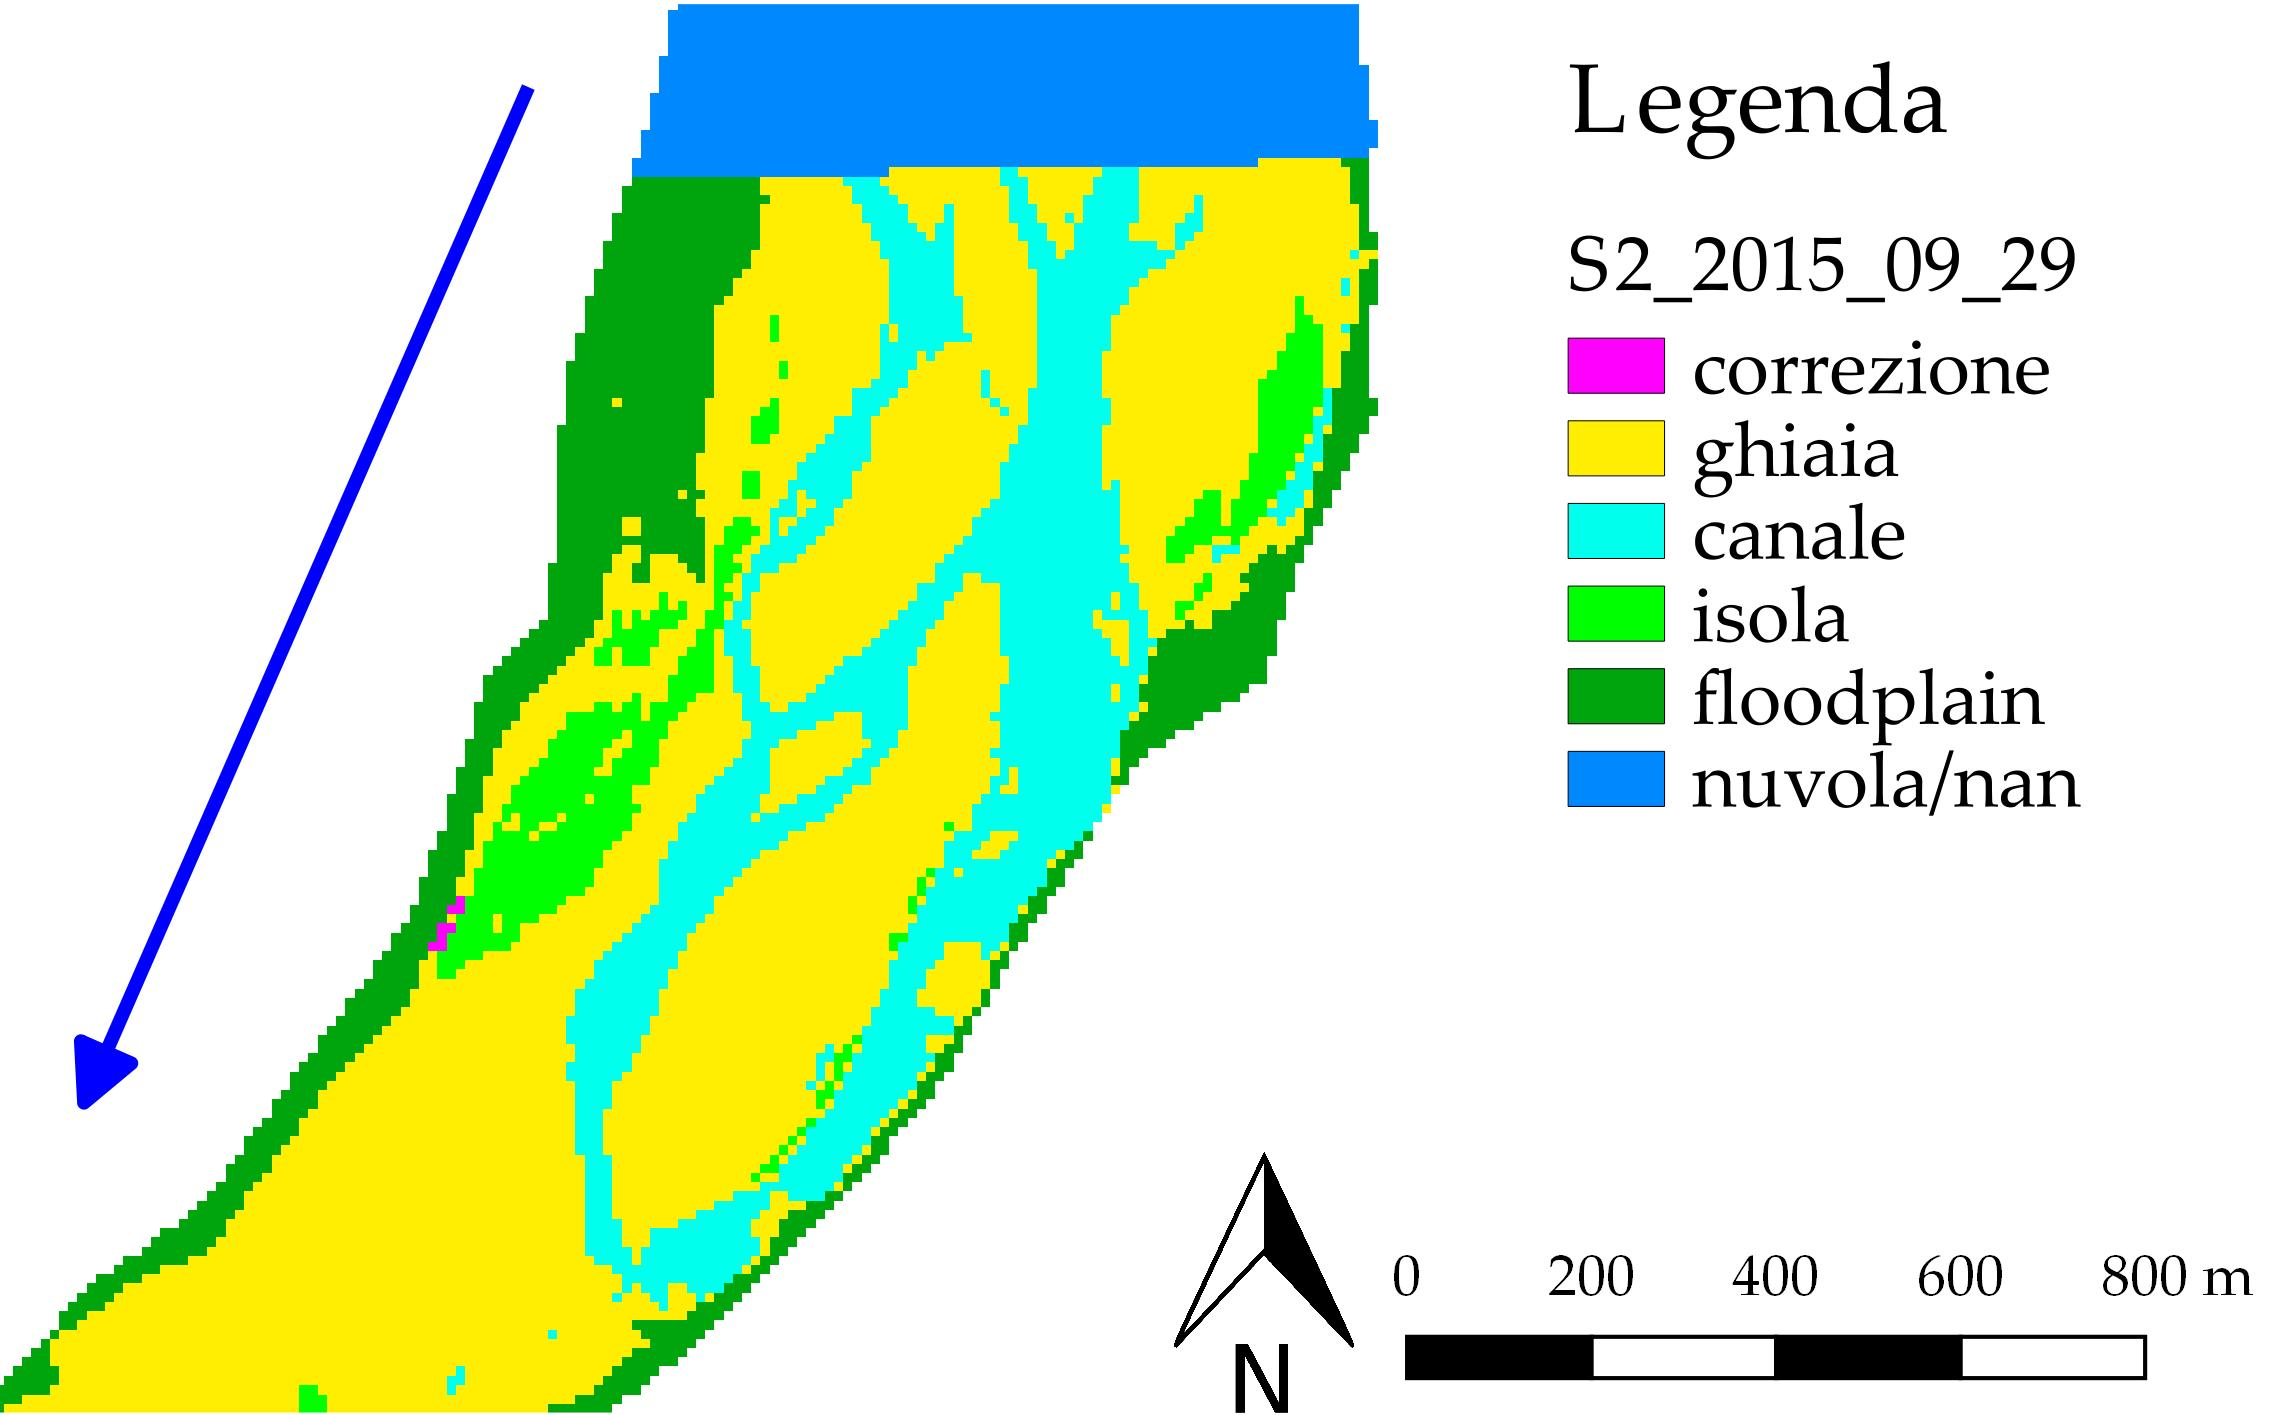
\includegraphics[width=\textwidth]{files/esempio_class_is_fl.jpeg}
		\caption[esempio della classificazione dell'area dei tratti]{esempio della classificazione dell'area dei tratti; le zone raffigurate sono rispettivamente a monte dell'isola di Cornino (in corrispondenza del monte Prat) e in corrispondenza della confluenza del Fella.}
		\label{fig:class_is_fl}
	\end{figure}
	%
Al fine di validare la precedente procedura di controllo e correzione della distinzione isole - \emph{floodplain}, si è osservato per ogni tratto l'andamento temporale della larghezza media~$B$, esprimibile semplicemente come il rapporto dell'area dell'alveo di ogni tratto (somma dell'alveo attivo e delle isole) per la sua lunghezza seguendo la corrente:
	%
	\begin{equation}
		\label{eq:larghezza-tratto}
		B = \frac{\text{Area alveo}}{Lunghezza} 
		\quad .
	\end{equation}
	% 
	Si è verificato che la larghezza~$B$ rimanesse costante nel tempo, indice di una corretta classificazione tra isole e \emph{floodplain}. 
	La~$B$ non rimane costante solo nel caso di distacco di isole o di fusione di isole nella piana. 
	\\
	La \cref{fig:b-media-7-e-15} mostra l'andamento temporale della~$B$ dei tratti~7 e~15: nel primo tratto, in cui non si osserva alcuna variazione sensibile dell'alveo, la~$B$ oscilla solo di qualche decina di metri; nel secondo si assiste alla progressiva fusione di una grande isola nella \emph{floodplain}, e questo lo si vede proprio nella diminuzione della~$B$. Ciò che conta non è quanto è largo l'alveo, ma quanto cambia la larghezza.
	%
	\begin{figure}
		\centering
		\begin{tikzpicture}
	\begin{axis}[
		width = 0.6\textwidth,
		height = 0.5\textwidth,
		date coordinates in = x,
		xticklabel = {\year},
		xticklabel style = {
			rotate = 80,
			anchor = near xticklabel
		},
		xtick distance = 730,
		enlarge x limits = 0.05,
		enlarge y limits = 0.01,
		%ymax = 3.7,
		%ymin = -0.1,
		%ytick distance = 0.5,
		ylabel = {Larghezza media dell'alveo \si{[\m]}},
		grid = major,
		]
		\addplot+
        	[blue]
        	table [x=data, y=tr_7] {graphics/data/Larghezze_medie_alveo.txt};
        \addlegendentry{Tratto 7}
        
		\addplot+
        	[orange]
        	table [x=data, y=tr_15] {graphics/data/Larghezze_medie_alveo.txt};
        \addlegendentry{Tratto 15}
	\end{axis}
\end{tikzpicture}

		\quad
		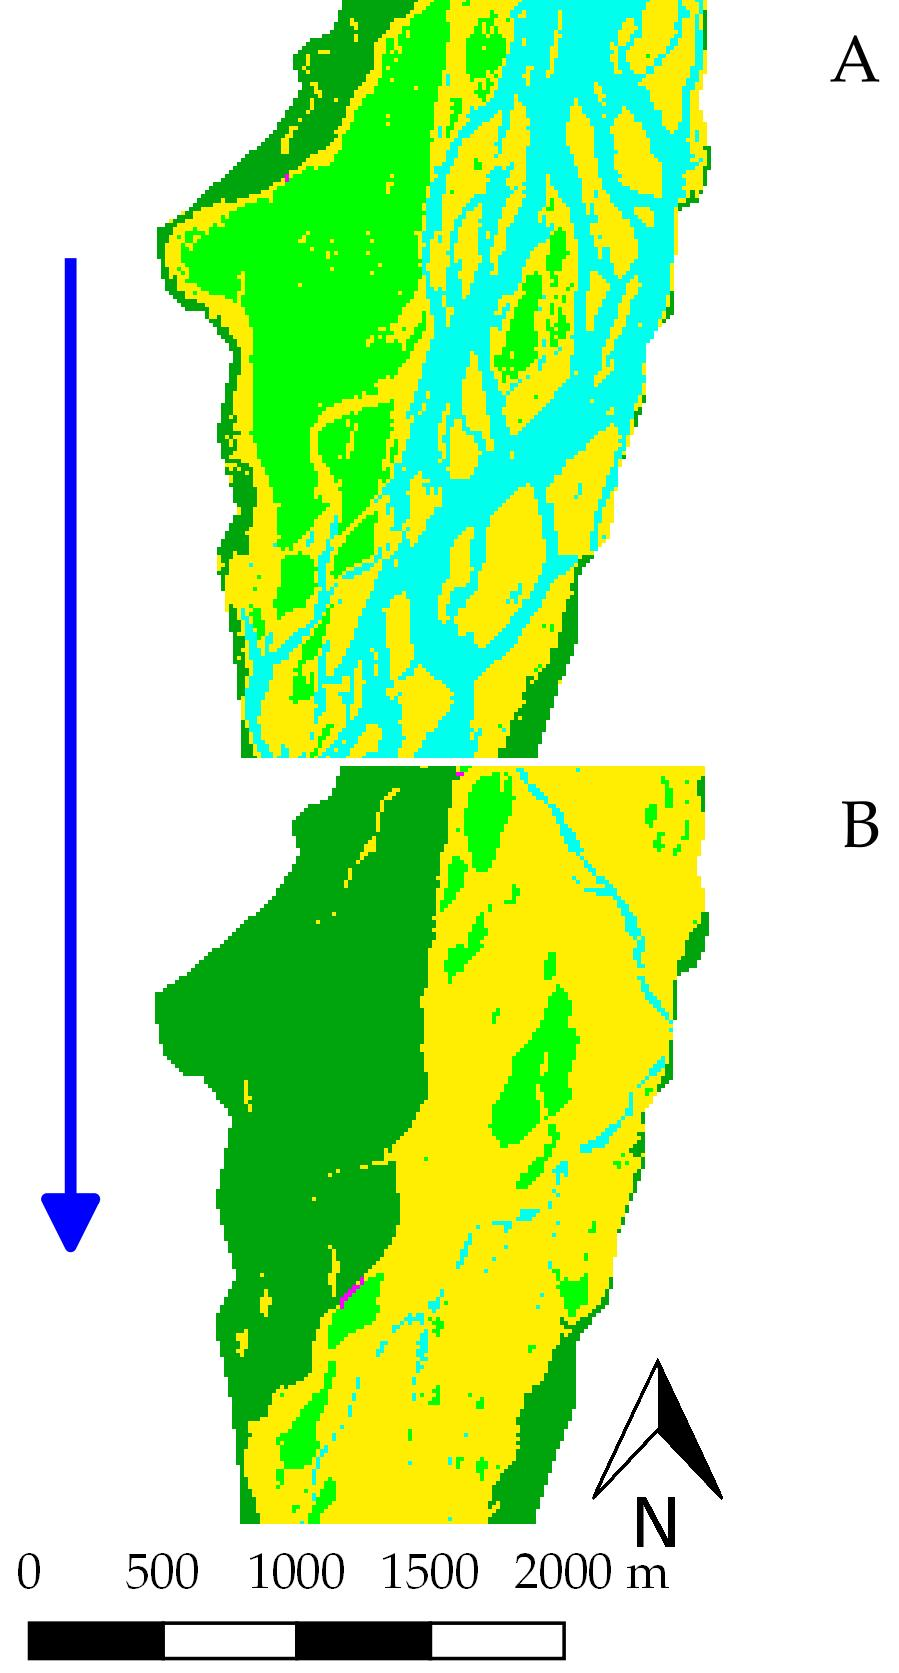
\includegraphics[width=0.3\textwidth]{files/fusione_isola_tr_15.jpeg}
		\caption[andamento temporale di $B$ per i tratti~7 e~15]{a sinistra si vede l'andamento nel tempo della larghezza media dei tratti~7 e~15; la $B$ del tratto~7 oscilla solamente di qualche decina di metri, mentre il tratto~15 riduce improvvisamente la sua $B$ a causa della fusione di una grande isola nella \emph{floodplain}, fenomeno mostrato a destra (A: 2002-06-12, B: 2005-08-30).}
		\label{fig:b-media-7-e-15}
	\end{figure}
	%
	%
	\item[Ulteriore validazione] Si è confrontata la classificazione del 2011-10-02 con la classificazione eseguita manualmente da \squarecite{Surian:2015} nei tratti \numrange[range-phrase={$\div$}]{6}{12} (dal ponte autostradale di Braulins alla stretta di Pinzano).
	Le mappe di classificazione del 2005-08-30, 2010-09-29, 2013-09-05 sono state confrontate con i CHM ricavati dai rilievi aerei LiDAR eseguiti nei corrispondenti anni sui tratti \numrange[range-phrase={$\div$}]{6}{12} (\cref{fig:validazione-class-is-fl}).
	Tra i rilievi LiDAR e le immagini \AST{} non hanno avuto luogo particolari eventi di piena.
	%	
	\begin{figure}
		\centering
		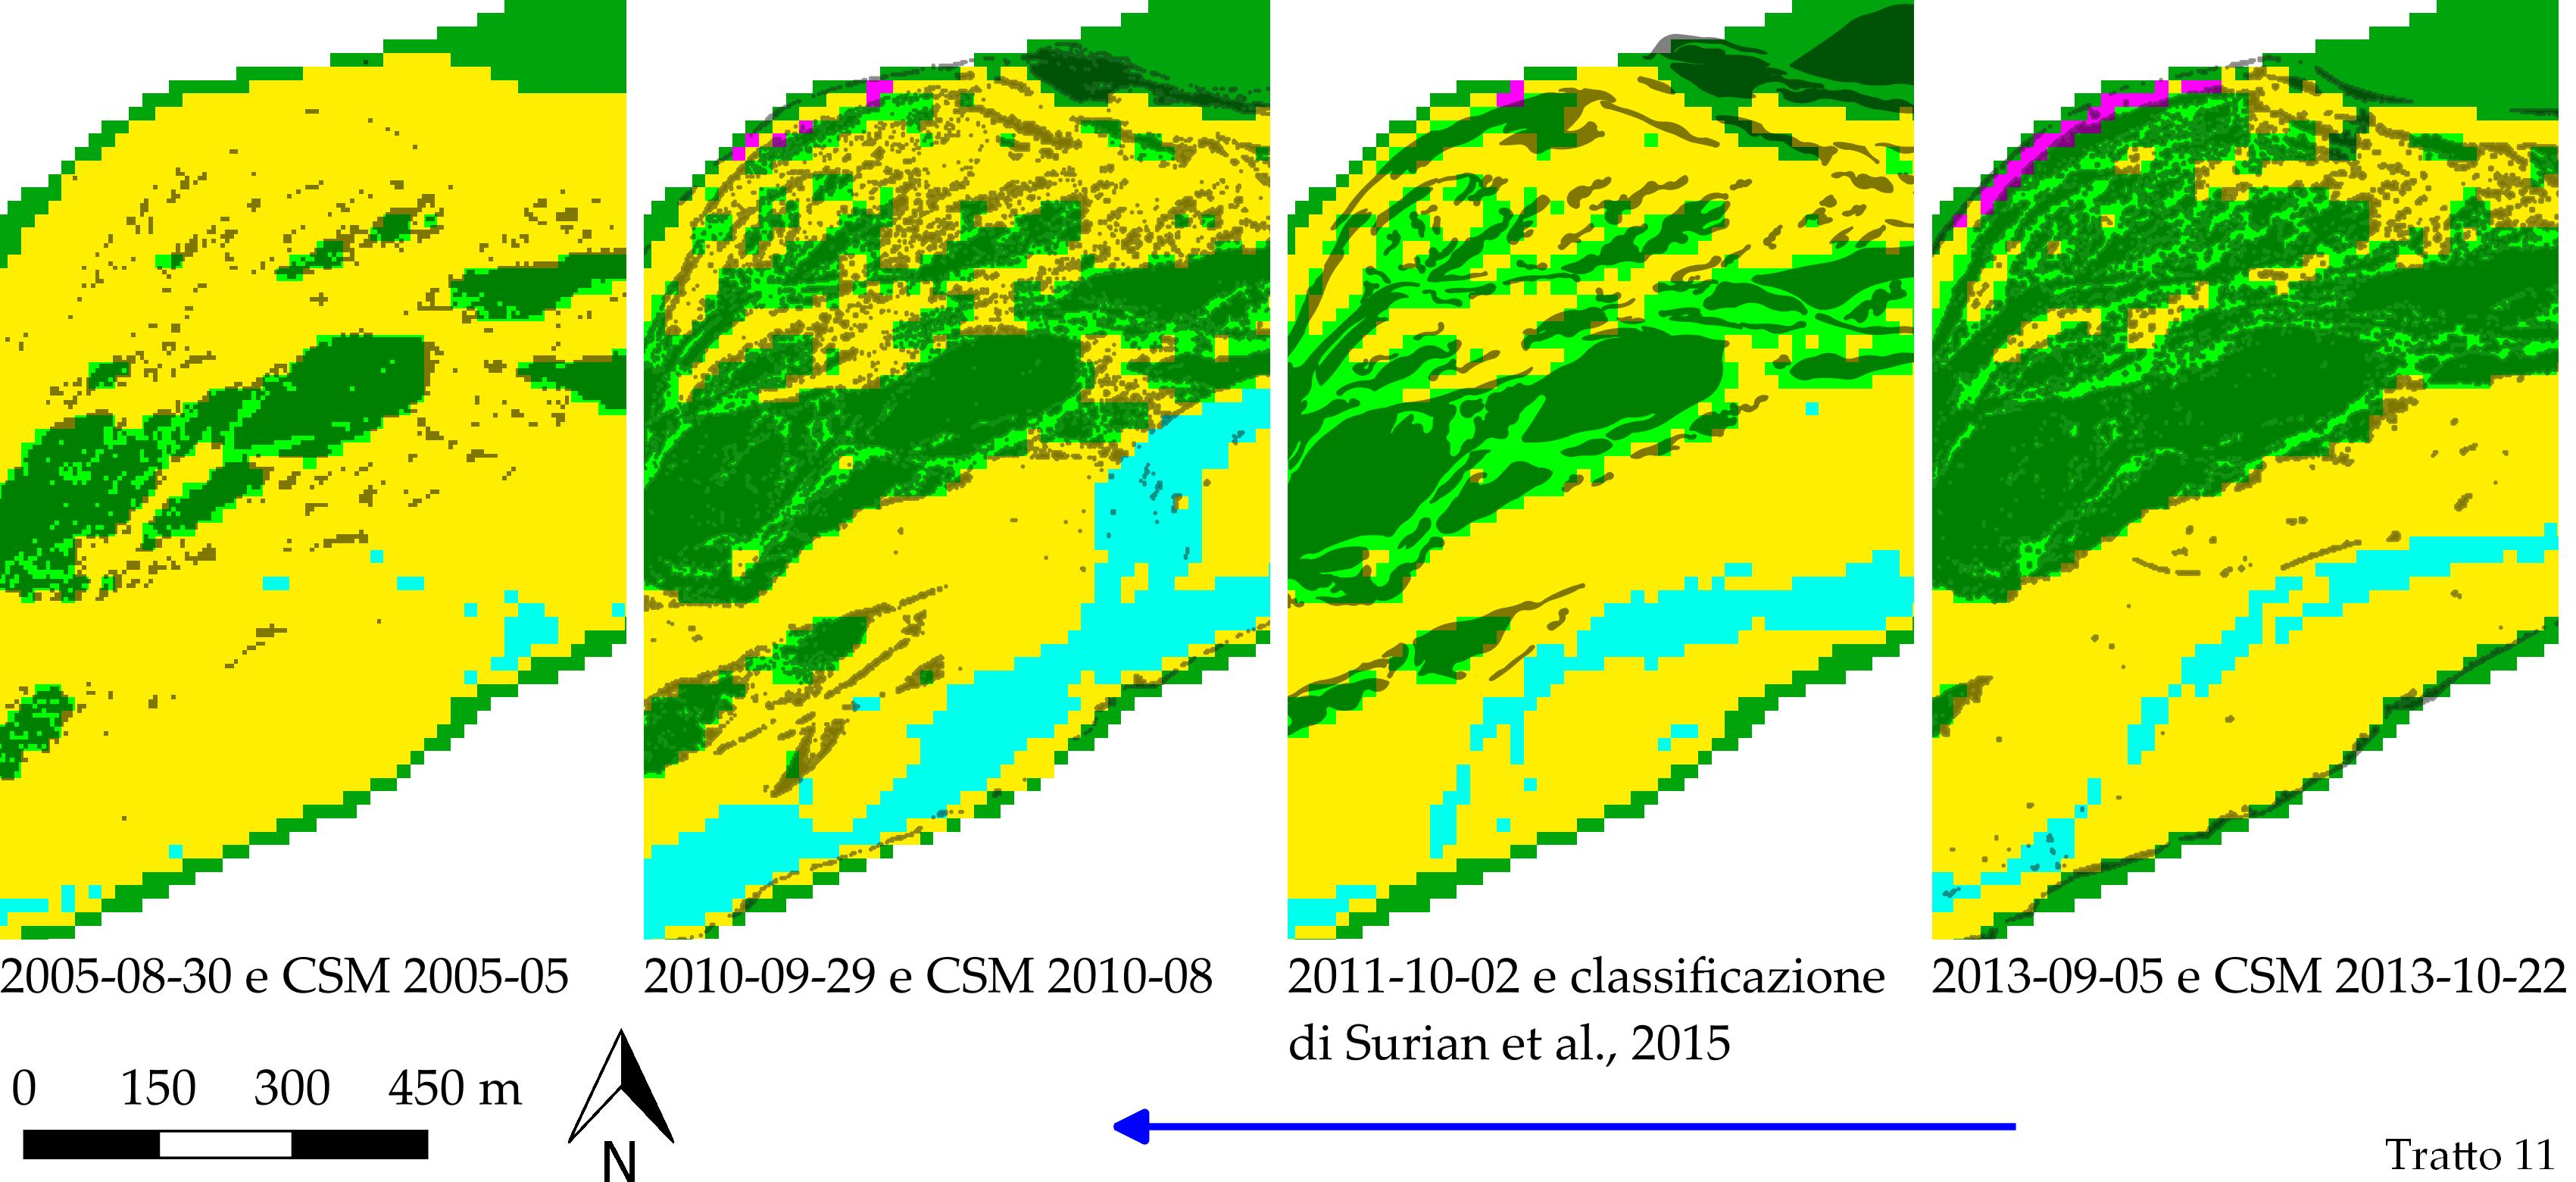
\includegraphics[width=\textwidth]{files/class_mia_vs_surian_chm.jpeg}
		\caption[validazione della classificazione dell'alveo]{confronto tra le mappe di classificazione dell'alveo e i CHM dai rilievi aerei LiDAR e la classificazione manuale eseguita in \squarecite{Surian:2015}; le aree scure corrispondono alla vegetazione individuata nei CHM e dalla classificazione manuale; per la legenda delle mappe di classificazione dell'alveo vedere la \cref{fig:class_is_fl}.}
		\label{fig:validazione-class-is-fl}
	\end{figure}
	%
	\\
	Visualmente si verifiche che c'è sostanziale corrispondenza tra le classificazioni ottenute dalle immagini satellitari e la vegetazione individuata dai CHM, così come tra la classificazione manuale di \squarecite{Surian:2015} e la mappa del 2011-10-22.
	\\
	Esiste una certa differenza tra la classificazione manuale e quella semi-automatica utilizzata nel presente lavoro: la metodologia con cui si procede influisce sul risultato finale.
	Avendo \squarecite{Surian:2015} utilizzato ortofoto ad alta risoluzione (\SI{0.1}{\m}), hanno potuto facilmente distinguere le chiome dei singoli alberi dalla ghiaia o vegetazione bassa circostante; le immagini satellitari utilizzate (principalmente a risoluzione di \SI{10}{\m} o \SI{15}{\m}) permettono invece di osservare macchie di vegetazione.
	In quanto si considera come isola non solo la vegetazione presente all'interno dell'alveo attivo, ma anche la zona meno vegetata posta circa alla medesima quota, l'approccio seguito sembra delineare più nettamente il contorno delle isole maggiori, sebbene le isole più piccole (con estensione minore di una cella) non siano individuate.
	\\
	Un rapido confronto delle mappe di classificazione \Pl{} e \WV{} ad alta risoluzione (\SI{0.5}{\m}) con le mappe di classificazione manuale e il CHM del 2013-10-22 mostra una sovrapposizione quasi completa della vegetazione individuata con i diversi metodi.
	\\
	A fronte di quanto esposto, si ritiene che la classificazione eseguita sia sufficientemente validata.
\end{description}


\begin{comment}
%TODO tenere questa parte? forse la si può togliere
% e mostrare direttamente i risultati sul cambiamento
Con la riclassificazione delle immagini dell'NDVI rispetto alle soglie proposte è stato possibile ottenere la percentuale di alveo coperta da vegetazione per ogni anno. 
Si ricorda, grazie alla maschera applicata, tale copertura include sia isole vegetate sia la parte di piana alluvionale che nel periodo di studio ha esperito fenomeni di erosione della vegetazione e quindi espansione dell'alveo attivo.
Infine, per le immagini l'alveo parzialmente coperto da nuvole, la maschera è stata estesa per escludere tali zone coperte poiché queste presentano valori di NDVI non corretti.
\\
I risultati sono mostrati nel grafico in \cref{graph:class-sat-veg}.


\begin{figure}[ht]
	\centering
	\begin{tikzpicture}
	\begin{axis}[
		width = \textwidth,
		height = 0.5\textwidth,
		date coordinates in = x,
		date ZERO = 2000-01-01,
		xticklabel = {\year},
		xticklabel style = {
			rotate = 80,
			anchor = near xticklabel
		},
		axis y line* = right,
		ymax = 70,
		%ymin = 0,
		ylabel = {Percentuale di vegetazione},
		grid = none,
		]
		\addplot+
        	[red, mark=+, ultra thick]
        	table [x=data, y=veg] {graphics/data/Class_sat_veg-H2O-ghiaia.txt};
	\end{axis}
	
	\begin{axis}[
		width = \textwidth,
		height = 0.5\textwidth,
		date coordinates in = x,
		date ZERO = 2000-01-01,
		xticklabel = {\year},
		xticklabel style = {
			rotate = 80,
			anchor = near xticklabel
		},
		axis y line* = left,
		axis x line = none,
		enlarge x limits = 0.05,
		enlarge y limits = 0.01,
		ymax = 3.7,
		ymin = 2,
		ylabel = {Livello idrometrico},
		grid = none,
		]
		\addplot+
        	[blue, no markers, ultra thin]
        	table [x=data, y=media-gg] {graphics/data/Dati_Villuzza.csv};
	\end{axis}
\end{tikzpicture}

	\caption[andamento dell'areale della vegetazione nelle isole  e nella floodplain]{andamento dell'areale della vegetazione nelle isole e nella floodplain (in rosso). I dati provengono dalla classificazione delle immagini satellitari (\AST{}, \Pl{}, \Se{} e \WV{}). In blu sono mostrati i livelli idrometrici medi giornalieri superiori a~\SI{2}{\m} registrati alla stazione di Villuzza.}
	\label{graph:class-sat-veg}
\end{figure}
% grafico piene 2m+ - %veg tratti (nuovo file comprensivo di tutti i tratti)
\end{comment}



\subsection{Risultati: evoluzione della larghezza}
Utilizzando le mappe di classificazione del terreno all'interno della maschera computazionale, si è ottenuta una larghezza media~$B$ secondo l'equazione~\eqref{eq:larghezza-tratto}.
%TODO \cref{eq:larghezza-tratto}. 
\\
Osservando la variazione temporale di~$B$ è possibile evincere delle traiettorie evolutive sia a livello di singolo tratto, sia a scala più ampia.
Inoltre, considerando la variazione spaziale (da monte verso valle) dell'areale delle isole, sono evidenti i pattern di \emph{upwelling} o \emph{downwelling} utilizzati durante la definizione dei 23~tratti.


\section{Cambiamento delle isole}
\label{sec:cambiamento}
A partire dalle mappe di classificazione dell'alveo, sono state ottenute mappe sul cambiamento che le isole hanno, o non hanno, esperito: erosione, crescita, fusione nella \emph{floodplain} o permanenza (nessun cambiamento).
Il risultato sono i dati di partenza per ricercare relazioni con gli eventi di piena.
\\
Per ottenere questi dati, ogni mappa è stata confrontata con quella temporalmente precedente.
\\
L'analisi si è focalizzata sulle isole, mentre si è esclusa la piana alluvionale.

\subsection{Metodi: ottenere il cambiamento}
\paragraph{Limitazioni} \label{par:camb-limiti}
Alcune mappe hanno una estensione limitata oppure presentano zone con copertura nuvolosa: ciò riduce il numero di confronti possibili per alcuni tratti. 
Dalle 23 immagini satellitari (si veda la \cref{tab:date-orto-sat}) si sono ottenute in media 20~immagini di confronto per tratto (\cref{tab:confronti}).

Inoltre, le immagini \AST{} non sono correttamente georeferenziate e non sono perfettamente sovrapponibili; l'entità di questo scostamento è dell'ordine di qualche cella.
Questo difetto è di grande importanza poiché per poter investigare l'evoluzione temporale delle isole occorre poter osservare nel tempo ogni cella; se questa si sposta da un'immagine alla successiva, il confronto non è più valido.
\\
La soluzione adottata è stata quella di traslare ogni mappa a nord, sud, est o ovest del numero di celle necessario per poterla sovrapporre alla mappa temporalmente precedente.
L'operazione è stata ripetuta per ogni confronto, per ogni tratto, ed è stata verificata visivamente.
Il massimo errore residuo è di 1~cella (\SI{15}{\m}) di scostamento in pochissime zone nei primi tratti (\numrange[range-phrase={ - }]{1}{4}); data la locale topografia montuosa si è preferito ridurre l'errore a tale entità e tenerlo sotto controllo piuttosto di distorcere la mappa con altre misure di georettifica.
L'entità di questo errore è accettabile poiché quasi tutte le isole hanno estensione maggiore di \SI{225}{\m\tothe{2}}.
\\
Le altre immagini sono invece correttamente georeferenziate.

Infine, per poter confrontare immagini a diversa dimensione di cella, come le \AST{} a~\SI{15}{\m} con le \Pl{} a~\SI{0.5}{\m}, è stato necessario ricampionare le immagini con la dimensione minore (ad esempio le \Pl{}) alla risoluzione di quelle a dimensione maggiore (le \AST{} o le \Se{}).
\\
Nel ricampionamento l'areale delle isole subisce un incremento o una riduzione, così come l'areale della ghiaia e delle altre classi in quanto nelle celle a dimensione maggiore sono presenti numerose celle a dimensione minore, ognuna con un valore diverso (\cref{fig:ricamp-explanation}).
%
\begin{figure}
	\centering
	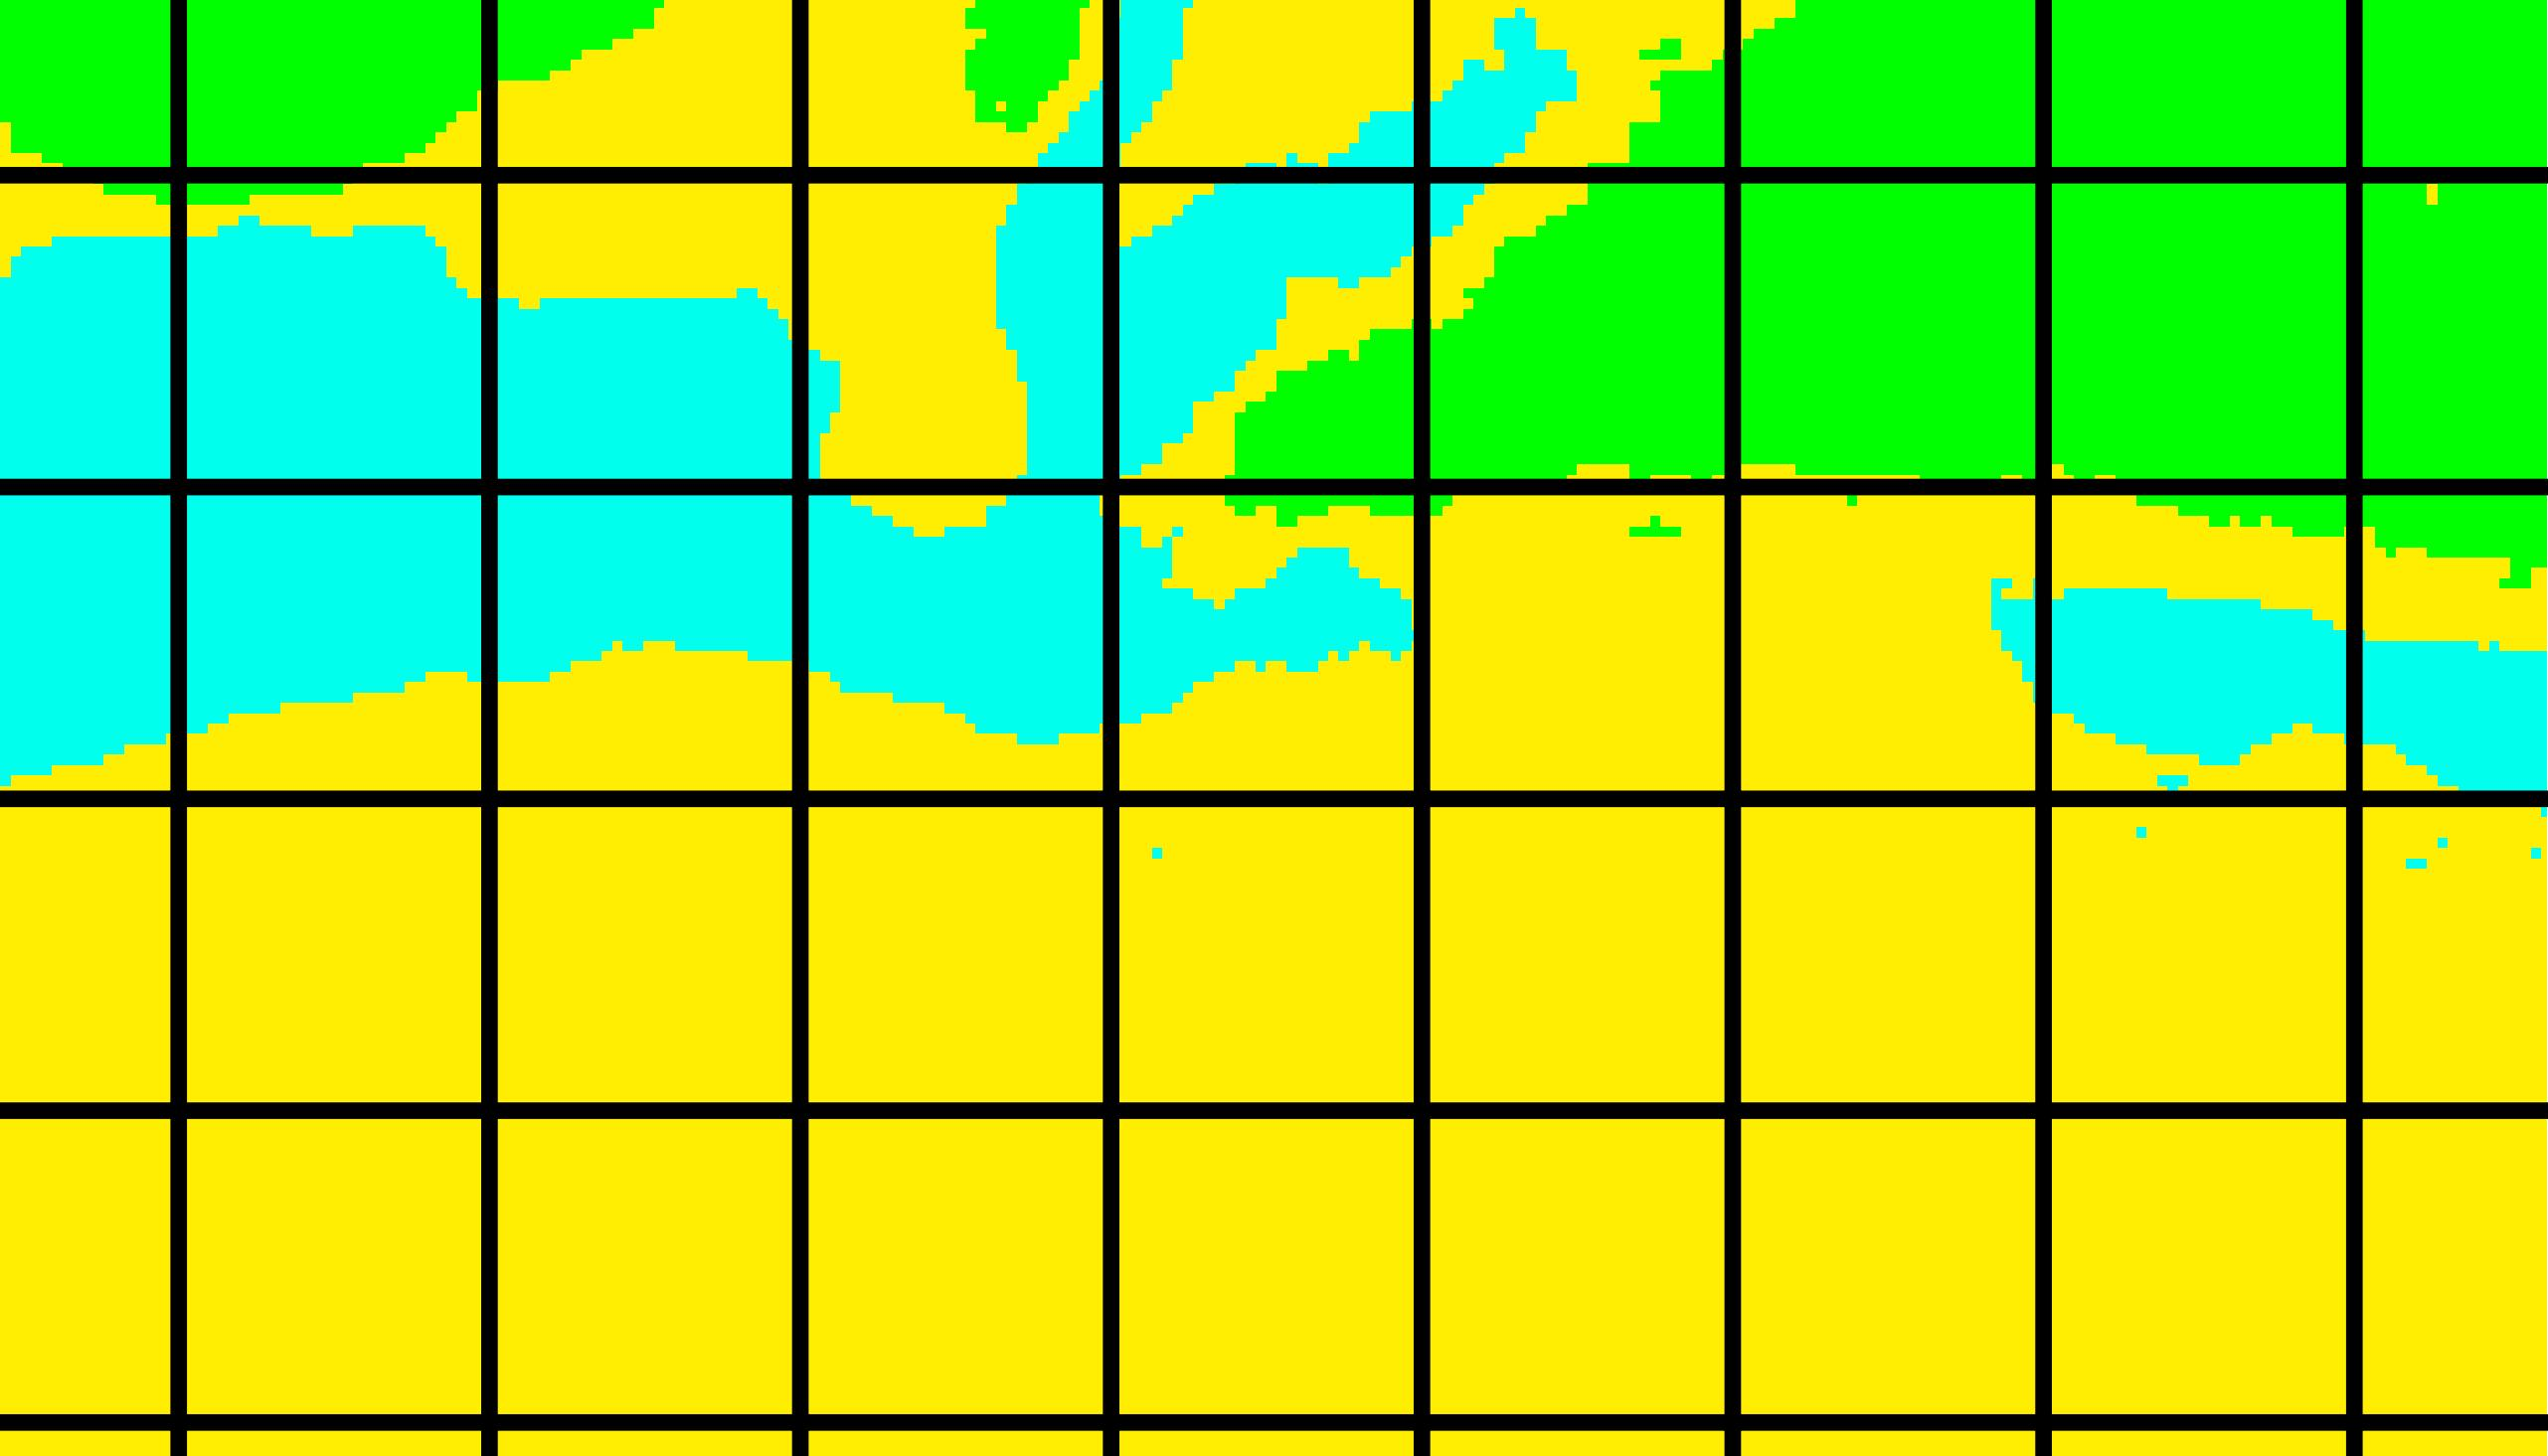
\includegraphics[width=.9\textwidth]{files/ricamp_griglia.jpeg}
	\caption[celle a risoluzione diversa]{immagine \Pl{} 2015-08-13 a~\SI{0.5}{\m} sullo sfondo con la griglia a~\SI{15}{\m} in primo piano; si vede come diverse celle più piccole siano contenute in una singola cella maggiore.}
	\label{fig:ricamp-explanation}
\end{figure}
%
Nel ricampionamento si sceglie quale valore assegnare alla nuova cella più grande in base ai valori delle celle minori; nel presente lavoro si è scelto di assegnare un percentile.
La scelta del percentile è stata effettuata confrontando la radice quadrata della somma dei quadrati residui (RSQR):
%
\begin{equation}
	\label{eq:rad-som-quad-res}
	RSQR = \left\lbrace \sum_{n=1}^{cl} \left[\left( \frac{area_{\mathrm{orig,n}}}{area_{\mathrm{orig,tot}}} - \frac{area_{\mathrm{perc,n}}}{area_{\mathrm{perc,tot}}} \right)^2 \right] \right\rbrace ^ \frac{1}{2}	
\end{equation}
%
dove 
\begin{itemize}
	\item $cl$ è il numero di classi (\cref{tab:class_tratti});
	\item $n$ indica la $n$-esima classe;
	\item $area_{\mathrm{orig,n}}$ e $area_{\mathrm{perc,n}}$ sono rispettivamente l'area della $n$-esima classe nella mappa originale e in quella ricampionata ad un percentile;
	\item $area_{\mathrm{orig,tot}}$ e $area_{\mathrm{perc,tot}}$ sono rispettivamente l'area totale della mappa originale e in quella ricampionata ad un percentile. 
\end{itemize} 
%
Si è scelto di normalizzare l'area di ogni classe per l'area totale per lavorare con percentuali.
\\
Nei ricampionamenti da \SI{0.5}{\m} il $50_\mathrm{mo}$ percentile (mediana) è quello che mostra il minor RSQR ($<\SI{3}{\percent}$). Un esempio del risultato ottenuto è mostrato in \cref{fig:ricampionamento}.
%
\begin{figure}
	\centering
	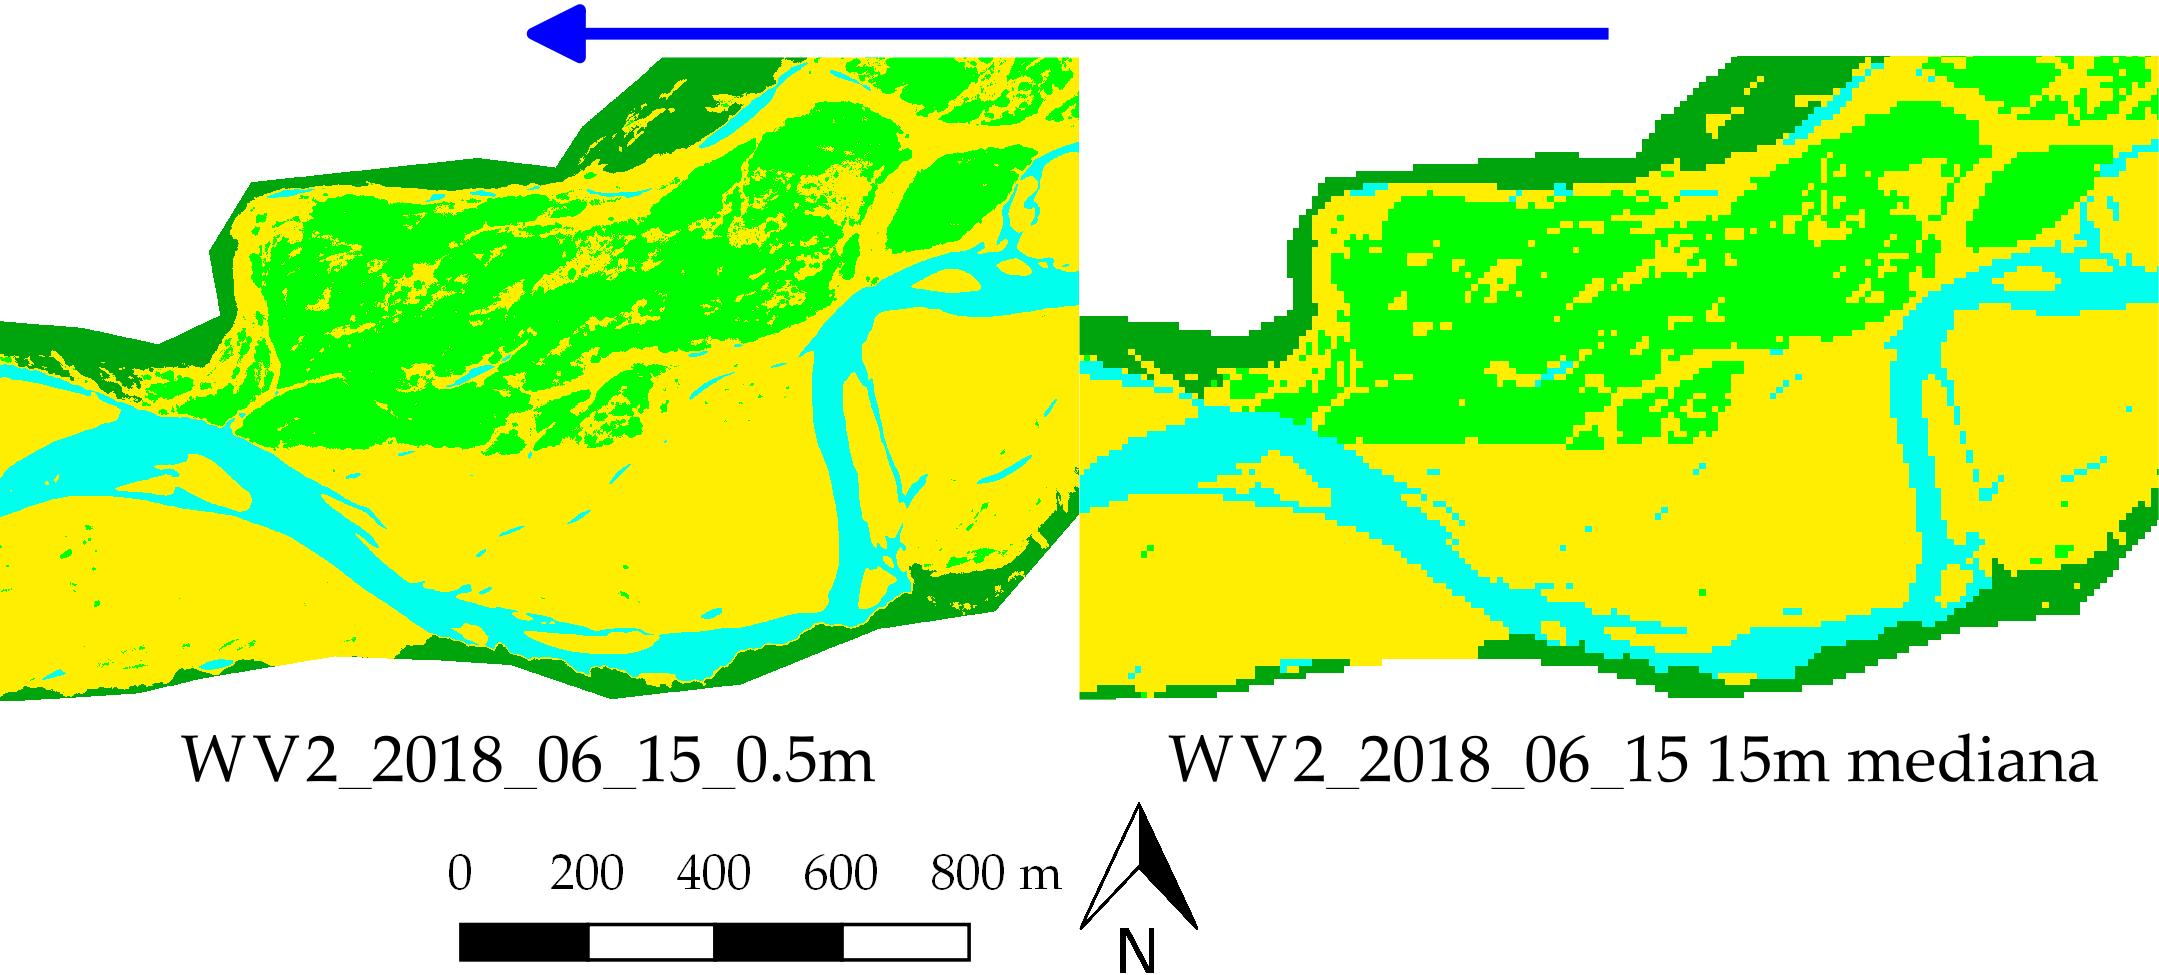
\includegraphics[width=\textwidth]{files/ricamp_class_is_fl.jpeg}
	\caption[confronto originale - ricampionamento]{a sinistra l'immagine \WV{} originale, poco a valle dell'isola di Cornino; a destra la stessa immagine ricampionata distribuendo i valori con la mediana.}
	\label{fig:ricampionamento}
\end{figure} 
%


\paragraph{Confronti validi}
Dalle 23 immagini satellitari è stato possibile ottenere il numero di confronti mostrati in \cref{tab:confronti}. 
I confronti effettuati hanno la massima risoluzione temporale possibile, cioè per ogni tratto si sono confrontate le immagini valide temporalmente più vicine in modo da poter osservare gli effetti cumulati del minor numero possibile di eventi di piena.
%
\begin{table}
	\centering
	\begin{tabular}{
		S[table-format=2.0] 
		S[table-format=2.0]
		c 
		c}
		\toprule
		\textbf{Tratto}	&	\textbf{Confronti}	&	\textbf{Primo}		&	\textbf{Ultimo}	\\
						&	\textbf{validi}		&	\textbf{confronto}	&	\textbf{confronto}	\\
		\midrule
		1	&	17	&	2000-09-17/2002-05-18	&	2017-09-13/2018-09-16	\\
		2	&	18	&	2000-09-17/2002-05-18	&	2017-09-13/2018-09-16	\\
		3	&	19	&	2000-09-17/2001-06-07	&	2017-09-13/2018-09-16	\\
		4	&	19	&	2000-09-17/2001-06-07	&	2017-09-13/2018-09-16	\\
		5	&	19	&	2000-09-17/2001-06-07	&	2017-09-13/2018-09-16	\\
		6	&	23	&	2000-09-17/2001-06-07	&	2018-06-15/2018-09-16	\\
		7	&	23	&	2000-09-17/2001-06-07	&	2018-06-15/2018-09-16	\\
		8	&	23	&	2000-09-17/2001-06-07	&	2018-06-15/2018-09-16	\\
		9	&	22	&	2000-09-17/2002-05-18	&	2018-06-15/2018-09-16	\\
		10	&	22	&	2000-09-17/2002-05-18	&	2018-06-15/2018-09-16	\\
		11	&	21	&	2000-09-17/2002-05-18	&	2018-06-15/2018-09-16	\\
		12	&	21	&	2000-09-17/2002-05-18	&	2018-06-15/2018-09-16	\\
		13	&	22	&	2000-09-17/2002-05-18	&	2018-06-15/2018-09-16	\\
		14	&	23	&	2000-09-17/2002-05-18	&	2018-06-15/2018-09-16	\\
		15	&	19	&	2000-09-17/2002-06-12	&	2017-09-13/2018-09-16	\\
		16	&	19	&	2000-09-17/2002-06-12	&	2017-09-13/2018-09-16	\\
		17	&	19	&	2000-09-17/2002-06-12	&	2017-09-13/2018-09-16	\\
		18	&	19	&	2000-09-17/2002-06-12	&	2017-09-13/2018-09-16	\\
		19	&	19	&	2000-09-17/2002-06-12	&	2017-09-13/2018-09-16	\\
		20	&	19	&	2000-09-17/2002-06-12	&	2017-09-13/2018-09-16	\\
		21	&	19	&	2000-09-17/2001-06-07	&	2017-09-13/2018-09-16	\\
		22	&	19	&	2001-06-07/2002-06-12	&	2017-09-13/2018-09-16	\\
		23	&	19	&	2001-06-07/2002-06-12	&	2017-09-13/2018-09-16	\\
		\bottomrule
	\end{tabular}
	\caption[confronti effettuati]{confronti effettuati con le 23 immagini satellitari a disposizione per ottenere dati sul cambiamento delle isole.}
	\label{tab:confronti}
\end{table}
%

\paragraph{Classi del cambiamento}
In ogni confronto ci si è concentrati sul ciò che è successo alle isole, definendo quindi le seguenti 4~classi (si veda anche la \cref{tab:class_tratti}):
%
\begin{itemize}
	\item erosione (da isola ad alveo attivo);
	\item crescita (da alveo attivo ad isola);
	\item fusione nella \emph{floodplain} (da isola a \emph{floodplain});
	\item distaccamento dalla \emph{floodplain} (da \emph{floodplain} a isola);
	\item nessun cambiamento (da isola a isola).
\end{itemize}
%
Un esempio di questa classificazione è riportato nella \cref{fig:confr-class-is-fl}.
%
\begin{figure}
	\centering
	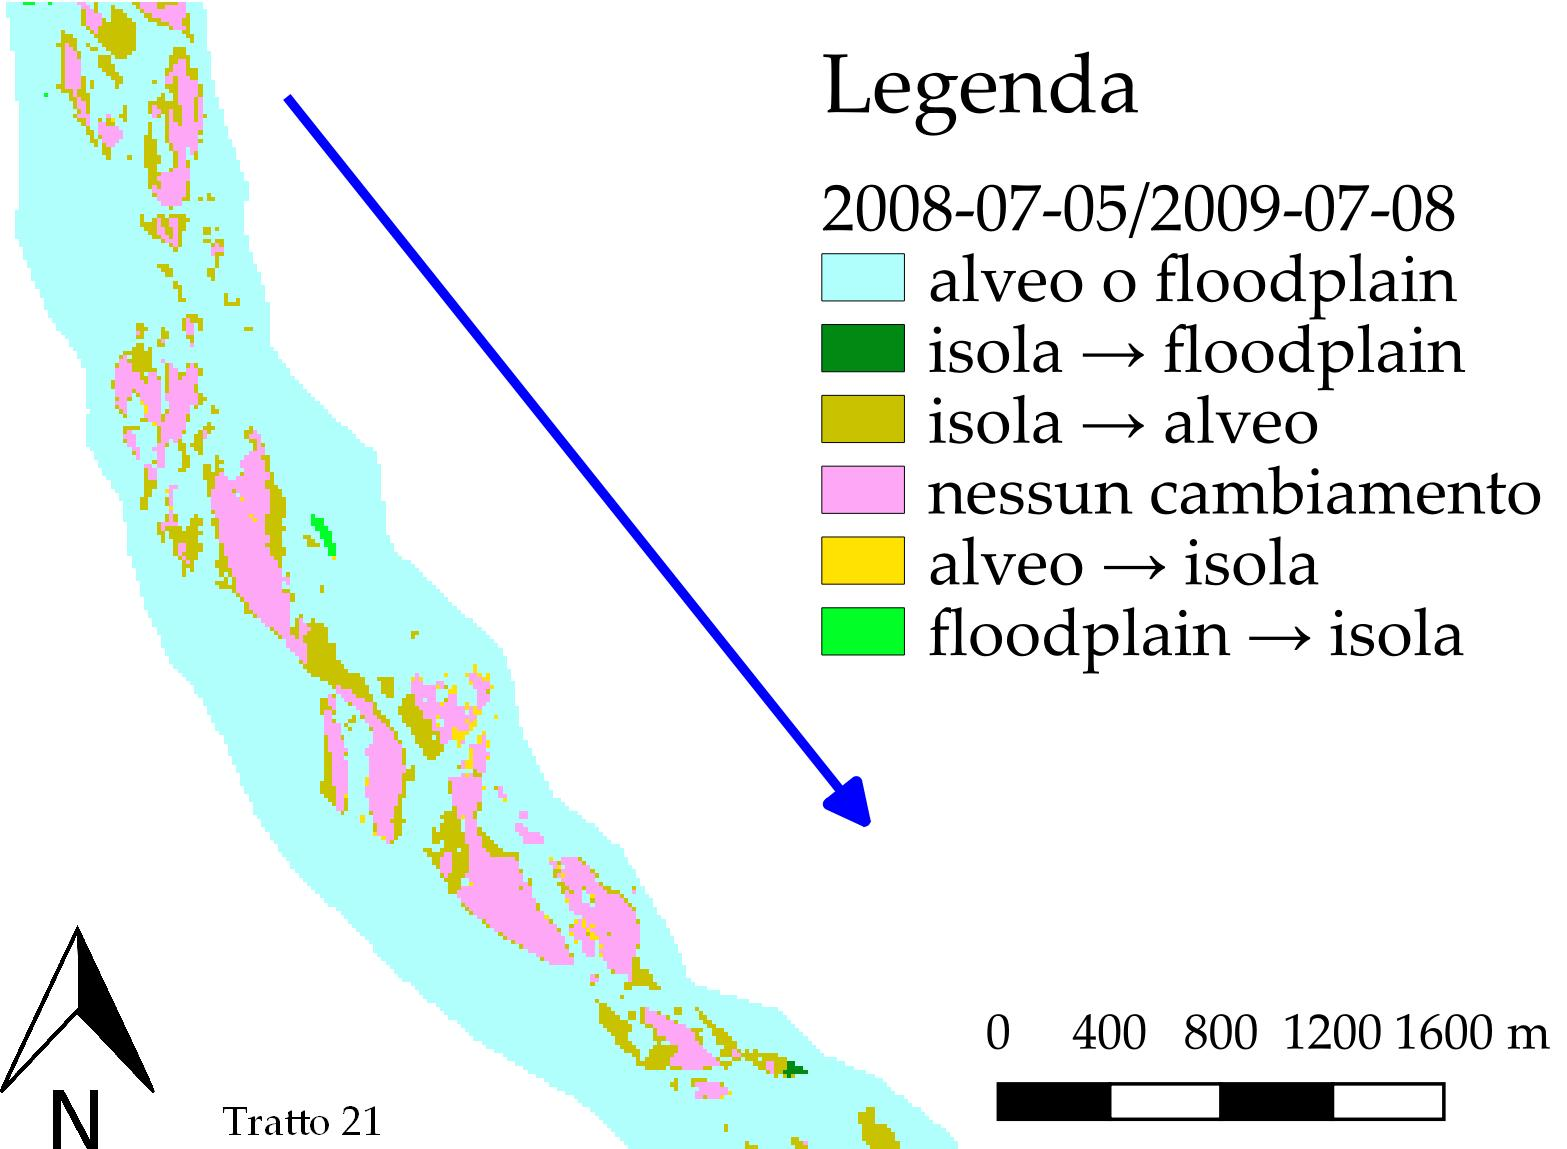
\includegraphics[width=.8\textwidth]{files/confr_class_is_fl.jpeg}
	\caption[esempio di mappa di cambiamento]{esempio di mappa di cambiamento ottenuta con il confronto tra le immagini \AST{} 2008-07-05 e 2009-07-08. Si possono osservare tutti i cambiamenti possibili; la prima classe serve solamente a visualizzare l'area della maschera computazionale. Il tratto mostrato è posto qualche \si{\kilo\m} a monte del ponte di Madrisio.}
	\label{fig:confr-class-is-fl}
\end{figure}
%


\subsection{Risultati: eventi eccezionali}
\label{sec:camb-ris}
Dall'osservazione dell'idrogramma in \cref{graph:livelli-matrix} e in \cref{graph:livelli-orto-sat} (riportato \cpageref{graph:tr-17-camb}) si può ipotizzare che le piene maggiori, come quelle avvenute verso la fine degli anni~2012 e~2014, siano quelle che abbiano asportato il maggior quantitativo di isole.
\\
I grafici in \cref{graph:tr-17-camb} mostrano alcuni risultati ottenuti dalle mappe di cambiamento per il tratto~17, posto nel tratto vallivo immediatamente a valle della confluenza con il torrente Cosa.
I dati sono rappresentati con due simboli: il pallino rappresenta la data finale di ogni confronto, mentre la croce indica la data iniziale; 
chiaramente il pallino di un confronto ha la stessa data della croce del confronto successivo. 
La croce serve solamente a sapere quanto dura ogni confronto; il pallino è il dato vero e proprio.
I dati sono normalizzati per l'areale delle isole nell'immagine \AST{} del 2000-09-17.
\\
Ciò che si vede è una spiccata crescita a cavallo degli anni~2006 e~2008, seguita da una erosione delle medesime proporzioni.
Dall'altra parte, nonostante la maggior intensità e durata le piene del 2012 e del~2014 hanno eroso meno di quanto ci si aspettava.
%
\begin{figure}
	\centering
	\begin{tikzpicture}
	%\begin{groupplot}
	\begin{axis}[
		%name = orto-sat,
		axis y line* = right,
		axis x line* = top,
		%height = .3\textwidth,
		width = \textwidth,
		date coordinates in = x,
		%symbolic y coords = {ASTER,PLEIADES,SENTINEL2,G-EARTH},
		xticklabel = {\year-\month-\day},
		xtick = data,
		ytick = data,
		xticklabel style = {
			rotate = 90,
			anchor = near xticklabel
		},
		enlarge x limits = 0.05,
		enlarge y limits = 0.01,
		ylabel = {Fonte},
		ymax = 3.6,
		ymin = -0.1,
		grid = none,
		only marks,
		]
		\addplot table [x=data, y=numero] {graphics/data/data-orto-sat.txt};
	\end{axis}
	%
	\begin{axis}[
		%name = stages,
		%at = {($(orto-sat.south)-(0,2cm)$)},
		%anchor = north,
		axis y line* = left,
		width = \textwidth,
		date coordinates in = x,
		xticklabel = {\year-\month-\day},
		xticklabel style = {
			rotate = 45,
			anchor = near xticklabel
		},
		enlarge x limits = 0.05,
		enlarge y limits = 0.01,
		ymax = 3.6,
		ymin = -0.1,
		ylabel = {Livello idrometrico},
		grid = major,
		no markers,
		]
		\addplot table [x=data, y=media-gg] {graphics/data/Dati_Villuzza.csv};
	\end{axis}
\end{tikzpicture}
	\\
	\begin{tikzpicture}
	\begin{groupplot}[
		group style = {
			group size = 2 by 1,
			ylabels at = edge left,
			x descriptions at = edge bottom,
			horizontal sep = 1.1cm,
			vertical sep = 0.1cm,
		},
		width = 0.5\textwidth,
		height = 0.5\textwidth,
		date coordinates in = x,
		xticklabel = {$\year$},
		xticklabel style = {
			rotate = 80,
			anchor = near xticklabel
		},
		xtick distance = 731,
		ymax = 0.75,
		ylabel = {Cambiamento/Isole iniziali \si{[\percent]}},%\si{[\m\tothe{2}]}},
		grid = major,
		]
	\nextgroupplot % tr_17_accrescimento
		\addplot+
        	[only marks, blue]
        	table [
        		x=data_fine, 
        		y expr=\thisrow{alv->is}/808650.0
        		] {graphics/data/tr_17_camb_eros_accr.txt};
		\addplot+
        	[only marks, mark=x, black]
        	table [
        		x=data_ini, 
        		y expr=\thisrow{alv->is}/808650.0
        		] {graphics/data/tr_17_camb_eros_accr.txt};
        \node [fill = white, draw = black, anchor = south west] 
        	at (axis description cs: 0.05,0.8) {Accr.};
	\nextgroupplot % tr_17_erosione
		\addplot+
        	[only marks, blue]
        	table [
        		x=data_fine, 
        		y expr=\thisrow{is->alv}/808650.0,
        		] {graphics/data/tr_17_camb_eros_accr.txt};
		\addplot+
        	[only marks, mark=x, black]
        	table [
        		x=data_ini, 
        		y expr=\thisrow{is->alv}/808650.0,
        		] {graphics/data/tr_17_camb_eros_accr.txt};
        \node [fill = white, draw = black, anchor = south west] 
        	at (axis description cs: 0.05,0.8) {Eros.};
	\end{groupplot}
\end{tikzpicture}

	\caption[cambiamenti esperiti dalle isole nel tratto~17]{cambiamenti esperiti dalle isole nel tratto~17 rappresentati come percentuale rispetto all'areale delle isole nel 2000-09-17. 
	Si nota il dato relativo al confronto 2008-07-05/2009-07-08, particolarmente elevato e di quasi pari entità tra crescita ed erosione.}
	\label{graph:tr-17-camb}
\end{figure}
%
Questa osservazione può trovare la seguente giustificazione: il periodo privo di piene con livello al disopra dei \SI{2}{\m} tra fine del 2004 e la fine del 2008 è stato favorevole per l'insediamento di nuova vegetazione;
le macchie vegetate sono diventate visibili da satellite solamente quando le piante hanno sviluppato una chioma sufficientemente ampia, cioè dopo qualche anno, nell'immagine del 2008-07-05;
questa più recente vegetazione si è espansa sulle barre e sulle forme morfologiche a quota minore rispetto alle isole più vecchie;
con questi fatti, la prima piena che è giunta ha facilmente portato via tutte queste isole giovani e basse.
\\
Occorre quindi ragionare non solo in termini di singoli eventi di piena, ma estendere le proprie considerazioni all'intero idrogramma, al periodo di tempo tra piene oltre un certo livello, alla loro frequenza, poiché sono questi i fattori che possono determinare le dinamiche delle isole.
Il periodo 2005-2008 privo di grandi piene può essere considerato un evento tanto importante quanto la piena lunga ed intensa del mese di Novembre, 2014.

%TODO c'è un trend: i tratti con upwelling sono quelli che si vegetano di più


Da queste osservazioni il passo successivo è naturale: trovare la composizione delle isole in termini di età e riflettere se è la vegetazione più giovane quella ad essere più facilmente erosa.



\section{Età della vegetazione nelle isole}
Utilizzando le mappe del cambiamento esperito dalle isole si possono ottenere mappe che indicano un'età approssimativa della vegetazione che compone queste isole. 
\\
L'ipotesi che si vuole verificare è che sia la vegetazione più giovane quella ad essere maggiormente erosa in quanto può essere divelta più facilmente.
Non si esclude tuttavia di osservare erosione anche di vegetazione matura poiché le isole poste in corrispondenza dell'estradosso di un canale in curva sono soggette a scavo laterale.

\subsection{Metodi: estendere i confronti e ottenere un'età}
\paragraph{Limiti}
Con le immagini satellitari utilizzate non è possibile distinguere i singoli alberi che compongono le isole; se con le immagini a miglior risoluzione si distinguono gli arbusti isolati, non si può certo ottenere una stima dell'età tanto precisa quanto quella fornita da un carotaggio del tronco.
In più, una cella è classificata come vegetazione solo quando le piante al suo interno presentano complessivamente una chioma sufficientemente grande da occupare gran parte della cella; pertanto le immagini con celle di \SI{10}{\m} o  \SI{15}{\m} non possono mostrare che grandi macchie di vegetazione.
Prima dei \SI{3}{\anni} una pianta di salice generalmente non ha fronde molto estese.
\\
Occorre poi tenere in conto che le piante crescono differentemente in base alle condizioni ambientali: periodi di stress idrico o termico rallentano la crescita, così come il parziale seppellimento con ghiaia dovuto ad eventi di piena; una falda non troppo profonda la cui altezza varia lentamente, terreno di granulometria sottile con sabbia e buone temperature sono invece fattori favorevoli alla crescita \squarecite{Gurnell:2001-island-formation}.

Si crede che ciò che possa generalmente accadere è che fino ad una certa età, circa \SI{3}{\anni}, la nuova vegetazione non sia visibile dal satellite; quindi si può definire come età della vegetazione presente in una cella la somma della persistenza (il periodo di tempo in cui si osserva che la cella rimane vegetata) con i \SI{3}{\anni} iniziali. 

Le mappe del cambiamento sono state ottenute dalle mappe di classificazione; non essendo le seconde correttamente georeferenziate, neanche le prime lo sono. L'errore residuo nel processo di correzione è di 1~cella.

Infine, per poter confrontare nel corso degli anni ogni cella, le mappe del cambiamento sono state ricampionate alla risoluzione più bassa, corrispondente a celle di~\SI{15}{\m} di lato. Si è proceduto come mostrato nel paragrafo \ref{par:camb-limiti} ottenendo sempre valori $RSQR < \SI{1.5}{\percent}$; i confronti a~\SI{10}{\m} sono stati ricampionati a~\SI{15}{\m} applicando il valore del $75_\mathrm{mo}$ percentile (terzo quartile).
 

%TODO le piante crescono diversamente in base alle condizioni ambientali (cita articolo Gurnell?) → definire un'età in base al tempo di osservazione è un approccio limitato (qualche altro lavoro simile)

\paragraph{Obiettivo ed approccio} 
Date le precedenti premesse, bisogna riflettere su ciò che si vuole ottenere: dividere la vegetazione in classi di età.
Si vuole sapere quanta vegetazione giovane è stata erosa; non conta se questa ha esattamente \SI{3}{\anni} o \SI{4}{\anni}, l'importante è che sia grossomodo classificata come giovane.

Ogni mappa del cambiamento è formata dalle informazioni contenute in due mappe: quella più vecchia e quella più recente. La distanza temporale tra queste due mappe definisce il periodo di osservazione.
\\
Per la mappa del cambiamento più vecchia (la prima mappa di confronto in \cref{tab:confronti}), l'età della vegetazione delle isole è stata scelta essere pari al periodo di osservazione, cui si sono aggiunti \SI{3}{\anni}, che è ritenuto il periodo minimo affinché un insieme di piante diventi visibile per il satellite.
\\
Per le mappe via via più recenti, l'età nelle celle delle isole che non sono cambiate è pari al periodo di osservazione sommato all'età precedente; per le celle si sono vegetate a partire dall'alveo l'età è pari al periodo di osservazione con l'aggiunta di \SI{3}{\anni}.

L'approccio di definire un'età in base al periodo di osservazione è limitato, in particolare per le mappe più vecchie, poiché non è possibile tener conto della vegetazione che era presente antecedentemente alla prima immagine valida;
si ritiene che a partire dalla $4^a$ o $5^a$ mappa di età il metodo inizi ad essere affidabile (generalmente quindi dalla mappa di età del 2007-09-21).
Per gli scopi della ricerca questo approccio risulta essere sufficiente.

\medskip
Si osservino i grafici in \cref{graph:distrib-rapp-eros-eta}, i quali rappresentano quante isole sono state erose rispetto alle isole presenti in ogni tratto in base all'età delle prime.
Si vede come le isole con età minore di \SI{5}{\anni} siano spesso erose; si evidenzia anche una dinamicità per le isole con età tra \SIrange[range-phrase={ e }]{5}{8}{\anni}. 
\\
Si definiscono quindi le seguenti classi di età:
%
\begin{itemize}
	\item giovane, con meno di \SI{5}{\anni};
	\item intermedia, con età compresa tra \SIrange[range-phrase={ e }]{5}{8}{\anni};
	\item matura, con più di \SI{8}{\anni}.
\end{itemize}
%
\begin{figure}
	\centering
	\tikzsetnextfilename{rapp_eros_eta}
\begin{tikzpicture}
	\begin{groupplot}[
		group style = {
			group size = 2 by 3,
			y descriptions at = edge left,
			x descriptions at = edge bottom,
			horizontal sep = 0.4cm,
			vertical sep = 0.4cm,
		},
		width = 0.54\textwidth,
		height = 0.54\textwidth,
		xlabel = {Età \si{[\anni]}},
		xmin = 3,
		xmax = 20,
		xtick distance = 3,
		enlarge x limits = 0.05,
		ylabel = {Isole erose / isole totali \si{[\percent]}},
		boxplot/draw direction = y,
		ymax = 70,
		ymin = 0,
		enlarge y limits = 0.05,
		grid = major,
	]
	\nextgroupplot % ASTER 2008_07_05
		\addplot [only marks]
			table [x=Eta, y=Perc_erosa_su_tot_isole] {graphics/data/rapp_eros_eta_2008_07_05.txt};
		\addplot [no markers, dashed, red]
			coordinates{(5,0) (5,70)};
		\addplot [no markers, dashed, red]
			coordinates{(8,0) (8,70)};
        \node [fill = white, draw = black, anchor = north east] 
        	at (axis description cs: 1,1) {AST 2008-07-05};
	%------------------------------------------------------
	\nextgroupplot % ASTER 2010_09_29
		\addplot [only marks]
			table [x=Eta, y=Perc_erosa_su_tot_isole] {graphics/data/rapp_eros_eta_2010_09_29.txt};
		\addplot [no markers, dashed, red]
			coordinates{(5,0) (5,70)};
		\addplot [no markers, dashed, red]
			coordinates{(8,0) (8,70)};
        \node [fill = white, draw = black, anchor = north east] 
        	at (axis description cs: 1,1) {AST 2010-09-29};
	%------------------------------------------------------
	\nextgroupplot % ASTER 2014_09_08
		\addplot [only marks]
			table [x=Eta, y=Perc_erosa_su_tot_isole] {graphics/data/rapp_eros_eta_2014_09_08.txt};
		\addplot [no markers, dashed, red]
			coordinates{(5,0) (5,70)};
		\addplot [no markers, dashed, red]
			coordinates{(8,0) (8,70)};
        \node [fill = white, draw = black, anchor = north east] 
        	at (axis description cs: 1,1) {AST 2014-09-08};
	%------------------------------------------------------
	\nextgroupplot % Sentinel2 2015_09_12
		\addplot [only marks]
			table [x=Eta, y=Perc_erosa_su_tot_isole] {graphics/data/rapp_eros_eta_2015_09_12.txt};
		\addplot [no markers, dashed, red]
			coordinates{(5,0) (5,70)};
		\addplot [no markers, dashed, red]
			coordinates{(8,0) (8,70)};
        \node [fill = white, draw = black, anchor = north east] 
        	at (axis description cs: 1,1) {S2 2015-09-12};
	%------------------------------------------------------
	\nextgroupplot % Sentinel2 2015_10_22
		\addplot [only marks]
			table [x=Eta, y=Perc_erosa_su_tot_isole] {graphics/data/rapp_eros_eta_2015_10_22.txt};
		\addplot [no markers, dashed, red]
			coordinates{(5,0) (5,70)};
		\addplot [no markers, dashed, red]
			coordinates{(8,0) (8,70)};
        \node [fill = white, draw = black, anchor = north east] 
        	at (axis description cs: 1,1) {S2 2015-10-22};
	%------------------------------------------------------
	\nextgroupplot % Sentinel2 2017_06_13
		\addplot [only marks]
			table [x=Eta, y=Perc_erosa_su_tot_isole] {graphics/data/rapp_eros_eta_2017_06_13.txt};
		\addplot [no markers, dashed, red]
			coordinates{(5,0) (5,70)};
		\addplot [no markers, dashed, red]
			coordinates{(8,0) (8,70)};
        \node [fill = white, draw = black, anchor = north east] 
        	at (axis description cs: 1,1) {S2 2017-06-13};
	\end{groupplot}
\end{tikzpicture}

	\caption[distribuzione del rapporto tra isole erose e la somma delle isole presenti]{distribuzione del rapporto tra le isole erose e la sommatoria di tutte le isole presenti per ogni tratto nei tratti da \numrange[range-phrase={ a }, mode=text]{1}{23} in base all'età; le linee verticali rosse tratteggiate indicano l'età di \SIrange[range-phrase={ e }]{5}{8}{\anni}.}
	\label{graph:distrib-rapp-eros-eta}
\end{figure}

\paragraph{Validazione}
Da un controllo visuale delle mappe di età si vede una corrispondenza tra struttura dell'età in diversi tipi di isole e quanto osservato da rilievi e osservazioni in campo \squarecite{Gurnell:2001-island-formation}: le isole complesse hanno una struttura d'età a macchie, quelle distaccate da floodplain uniforme (\cref{fig:struttura-eta}).
%
\begin{figure}
	\centering
	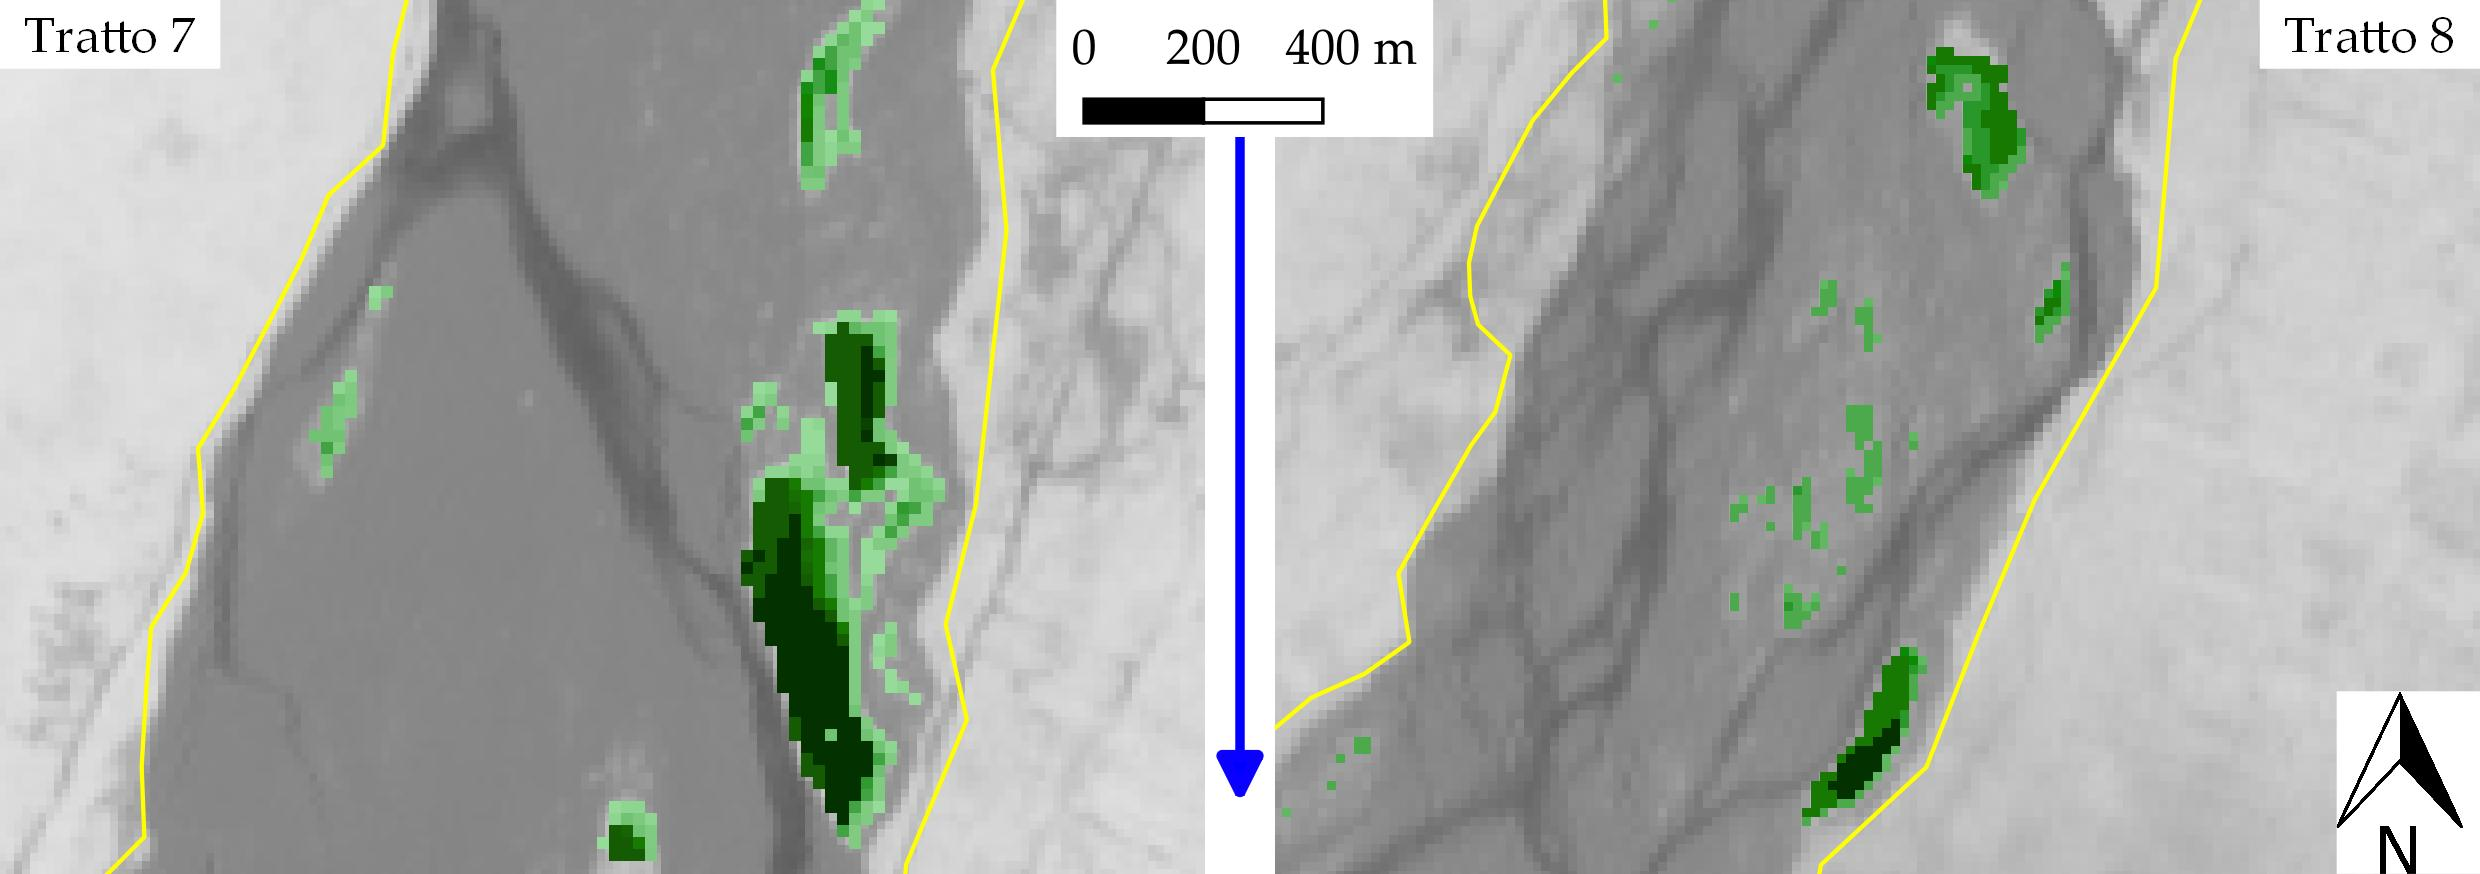
\includegraphics[width = \textwidth]{files/struttura_eta.jpeg}
	\caption[mappe della struttura di età in due tratti]{mappe della struttura di età in due tratti; i colori più scuri indicano una maggiore età.
		Nel tratto~7 (2017-06-13) si vede la struttura a macchie dell'età della vegetazione nelle isole complesse;
		nel tratto~8 (2009-07-08) si osserva la distribuzione più unifome dell'età nell'isola in basso, che si è formata dalla \emph{floodplain}.
		La maschera computazionale è mostrata in giallo; sullo sfondo sono mostrate le mappe NDVI.}
	\label{fig:struttura-eta}
\end{figure}
%

Il CHM (\emph{Canopy Height Model}) è il modello digitale della copertura arborea; similmente al DEM, mostra delle quote; queste sono tuttavia riferite all'altezza della vegetazione sopra il terreno.
\\
È generalmente sensato affermare che piante più mature abbiano un'altezza maggiore di piante giovani.
Quindi si sono utilizzati i dati di altezza della copertura arborea contenuti nei CHM di agosto~2010 e del~2013-10-22 per verificare che nelle celle della mappa di età della vegetazione rispettivamente del~2010-09-29 e del~2013-09-05 l'altezza fosse all'incirca proporzionale all'età.
Tra le date di ottenimento dei CHM e delle immagini \AST{} non vi sono stati eventi idrologici rilevanti.
I CHM sono stati ricampionati a \SI{15}{\m} (larghezza delle celle delle immagini \AST{}) applicando il valore del $75_{\mathrm{mo}}$ percentile in quanto rappresenta l'altezza delle chiome più elevate ed espanse, le quali dovrebbero definire i valori di età nelle mappe essendo maggiormente visibili da satellite.
\\
Si è scelto di validare la procedura solo sulle mappe di età del~2010 e del~2013 poiché sono più rappresentative della reale distribuzione d'età delle piante, mentre la mappa di età del 2005-08-30 potrebbe non essere affidabile per quanto precedentemente esposto.
\\
I \emph{boxplot} della distribuzione dell'altezza della vegetazione rispetto all'età sono presentati nel grafico in \cref{graph:altezza-chm-eta}.
Il loro andamento crescente riflette sufficientemente quello dei dati da rilievi dendrometrici effettuati da \squarecite{Gurnell:2018-canopy-height} su isole pioniere nel Tagliamento localizzate nei medesimi tratti del CHM; pertanto ci si ritiene soddisfatti della procedura sviluppata in quanto riesce ad ottenere una stima dell'età delle piante nelle isole adeguata agli scopi della tesi.
%
\begin{figure}
	\centering
	\tikzsetnextfilename{percentili_CHM_eta}
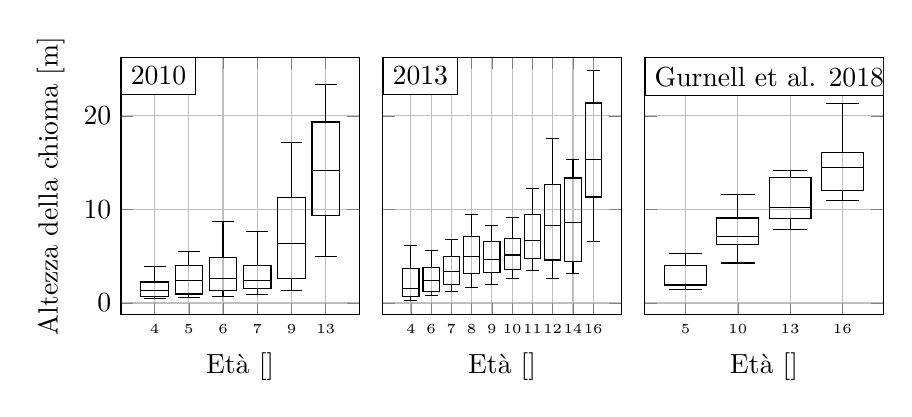
\begin{tikzpicture}
	\begin{groupplot}[
		group style = {
			group size = 3 by 1,
			y descriptions at = edge left,
			x descriptions at = edge bottom,
			horizontal sep = 0.3cm,
			vertical sep = 0.1cm,
		},
		width = 0.38\textwidth,
		height = 0.4\textwidth,
		xlabel = {Età \si{[\anni]}},
		xticklabel style = {font=\tiny},
		ylabel = {Altezza della chioma \si{[\m]}},
		boxplot/draw direction = y,
		ymax = 25,
		ymin = 0,
		enlarge y limits = 0.05,
		grid = major,
	]
	\nextgroupplot[
		xtick = {1, 2, 3, 4, 5, 6},
		xticklabels = {$4$, $5$, $6$, $7$, $9$, $13$},
		] % CSM età 2010
		\addplot [
			boxplot prepared = {
				lower whisker=0.44979499999999994,
				lower quartile=0.706821,
				median=1.349386,
				upper quartile=2.248977,
				upper whisker=3.919646,
				}
			]
			coordinates{};
		\addplot [
			boxplot prepared = {
				lower whisker=0.578308,
				lower quartile=0.963847,
				median=2.37749,
				upper quartile=4.048159,
				upper whisker=5.461802,
				}
			]
			coordinates{};
		\addplot [
			boxplot prepared = {
				lower whisker=0.706821,
				lower quartile=1.349386,
				median=2.634516,
				upper quartile=4.819237,
				upper whisker=8.700328600000006,
				}
			]
			coordinates{};
		\addplot [
			boxplot prepared = {
				lower whisker=0.9252931000000002,
				lower quartile=1.51002725,
				median=2.37749,
				upper quartile=4.0160307500000005,
				upper whisker=7.5951168,
				}
			]
			coordinates{};
		\addplot [
			boxplot prepared = {
				lower whisker=1.349386,
				lower quartile=2.634516,
				median=6.361392,
				upper quartile=11.244886,
				upper whisker=17.156482,
				}
			]
			coordinates{};
		\addplot [
			boxplot prepared = {
				lower whisker=4.94775,
				lower quartile=9.3814475,
				median=14.200684,
				upper quartile=19.341203,
				upper whisker=23.350807599999996,
				}
			]
			coordinates{};
		\node [fill = white, draw = black, anchor = north west] 
        	at (axis description cs: 0,1) {2010};
	%------------------------------------------------------
	\nextgroupplot[
		xtick = {1, 2, 3, 4, 5, 6, 7, 8, 9, 10},
		xticklabels = {$4$, $6$, $7$, $8$, $9$, $10$, $11$, $12$, $14$, $16$},
		] % CSM età 2013
		\addplot [
			boxplot prepared = {
				lower whisker=0.304544,
				lower quartile=0.657206,
				median=1.597636,
				upper quartile=3.713603,
				upper whisker=6.1352108000000065,
				}
			]
			coordinates {};
		\addplot [
			boxplot prepared = {
				lower whisker=0.774759,
				lower quartile=1.244974,
				median=2.420512,
				upper quartile=3.831157,
				upper whisker=5.594463,
				}
			]
			coordinates {};
		\addplot [
			boxplot prepared = {
				lower whisker=1.244974,
				lower quartile=1.950297,
				median=3.360942,
				upper quartile=5.006695,
				upper whisker=6.770001,
				}
			]
			coordinates {};
		\addplot [
			boxplot prepared = {
				lower whisker=1.6211462,
				lower quartile=3.125835,
				median=5.006695,
				upper quartile=7.122662,
				upper whisker=9.4972484,
				}
			]
			coordinates {};
		\addplot [
			boxplot prepared = {
				lower whisker=1.950297,
				lower quartile=3.243388,
				median=4.654033,
				upper quartile=6.534893,
				upper whisker=8.262933799999999,
				}
			]
			coordinates {};
		\addplot [
			boxplot prepared = {
				lower whisker=2.65562,
				lower quartile=3.59605,
				median=5.124248,
				upper quartile=6.9169435,
				upper whisker=9.097565300000001,
				}
			]
			coordinates {};
		\addplot [
			boxplot prepared = {
				lower whisker=3.478496,
				lower quartile=4.71281,
				median=6.652447,
				upper quartile=9.4149605,
				upper whisker=12.2009848,
				}
			]
			coordinates {};
		\addplot [
			boxplot prepared = {
				lower whisker=2.65562,
				lower quartile=4.5952565,
				median=8.2982,
				upper quartile=12.706465999999999,
				upper whisker=17.608457000000005,
				}
			]
			coordinates {};
		\addplot [
			boxplot prepared = {
				lower whisker=3.125835,
				lower quartile=4.418926,
				median=8.592084,
				upper quartile=13.35301175,
				upper whisker=15.351425,
				}
			]
			coordinates {};
		\addplot [
			boxplot prepared = {
				lower whisker=6.570159200000001,
				lower quartile=11.3252095,
				median=15.351425,
				upper quartile=21.3760555,
				upper whisker=24.8027469,
				}
			]
			coordinates {};
		\node [fill = white, draw = black, anchor = north west] 
        	at (axis description cs: 0,1) {2013};
	%------------------------------------------------------
	\nextgroupplot[
		xtick = {1, 2, 3, 4},
		xticklabels = {$5$, $10$, $13$, $16$},
		]
		\addplot [
			boxplot prepared = {
				lower whisker=1.46,
				lower quartile=1.9,
				median=1.96,
				upper quartile=3.99,
				upper whisker=5.25,
				}
			]
			coordinates {};
		\addplot [
			boxplot prepared = {
				lower whisker=4.27,
				lower quartile=6.23,
				median=7.06,
				upper quartile=9.08,
				upper whisker=11.61,
				}
			]
			coordinates {};
		\addplot [
			boxplot prepared = {
				lower whisker=7.85,
				lower quartile=8.99,
				median=10.25,
				upper quartile=13.42,
				upper whisker=14.12,
				}
			]
			coordinates {};
		\addplot [
			boxplot prepared = {
				lower whisker=10.92,
				lower quartile=12.06,
				median=14.46,
				upper quartile=16.11,
				upper whisker=21.30,
				}
			]
			coordinates {};
		\node [fill = white, draw = black, anchor = north west] 
        	at (axis description cs: 0,1) {Gurnell et al. 2018};
	\end{groupplot}
\end{tikzpicture}

	\caption[distribuzione dell'altezza delle piante secondo l'età]{distribuzione dell'altezza delle piante (dal CHM) secondo l'età (dalle mappe di età) per il 2010 e il 2013 confrontati con rilievi dendrometrici presentati da \squarecite{Gurnell:2018-canopy-height}.}
	\label{graph:altezza-chm-eta}
\end{figure}
%

\subsection{Risultati: un trend per la vegetazione erosa}
Osservando la distribuzione del rapporto tra isole erose e isole presenti rispetto all'età, sono state definite 3~classi di età della vegetazione:
%
\begin{itemize}
	\item giovane, con meno di \SI{5}{\anni};
	\item intermedia, con età compresa tra \SIrange[range-phrase={ e }]{5}{8}{\anni};
	\item matura, con più di \SI{8}{\anni}.
\end{itemize}
%
Si considerino le isole presenti in alcuni tratti e alcune immagini divise per classi di età; si considerino anche le isole erose in seguito alle immagini di cui sopra, divise per classi di età e nei medesimi tratti: ciò che si vede nel grafico in \cref{graph:distr-eta} è la quantità di isole erose per ogni classe rispetto alle isole presenti. 
%
\begin{figure}
	\centering
	\tikzsetnextfilename{eta_tratti_8_11_17}
\begin{tikzpicture}
	\begin{groupplot}[
		group style = {
			group size = 3 by 1,
			x descriptions at = edge bottom,
			y descriptions at = edge left,
			xticklabels at = all,
			horizontal sep = 0.2cm,
			vertical sep = 0.25cm,
		},
		width = 0.37\textwidth,
		height = 0.8\textwidth,
	    xbar stacked,
		enlarge x limits = 0.02,
		enlarge y limits = 0.10,
		symbolic y coords = {
			2008-07-05, 2009-07-08, 
			2012-08-01, 2013-09-05,  
			2016-09-13, 2017-06-13
		},
		ytick distance = 1,
		%scaled x ticks = false,
		xlabel = {Areale \si{[\m\tothe{2}]}},
		xmajorgrids = true,
		]
		\nextgroupplot % tratto_8
			\addplot[bar shift = .4cm, pattern = north east lines]
		       	table [y=data, x=giovane-e] {graphics/data/tr_8_eta.txt};
			\addplot[bar shift = .4cm, fill = green]
		       	table [
		       		y=data, 
		       		x expr=\thisrow{giovane} - \thisrow{giovane-e}
		       		] {graphics/data/tr_8_eta.txt};
		       		
			\resetstackedplots
			\addplot[bar shift = 0cm, pattern = north east lines, forget plot]
		       	table [y=data, x=interm-e] {graphics/data/tr_8_eta.txt};
			\addplot[bar shift = 0cm, fill = green!75!black]
		       	table [
		       		y=data, 
		       		x expr=\thisrow{interm} - \thisrow{interm-e}
		       		] {graphics/data/tr_8_eta.txt};
		       		
			\resetstackedplots
			\addplot[bar shift = -.4cm, pattern = north east lines, forget plot]
		       	table [y=data, x=matura-e] {graphics/data/tr_8_eta.txt};
			\addplot[bar shift = -.4cm, fill = green!40!black]
		       	table [
		       		y=data, 
		       		x expr=\thisrow{matura} - \thisrow{matura-e}
		       		] {graphics/data/tr_8_eta.txt};
		    
        	\node [fill = white, draw = black, anchor = north east] 
        		at (axis description cs: 1,1) {Tr. 8};
        %
		\nextgroupplot [% tratto_11
			legend style = {
				at = {(0.5,1.02)},
				legend columns = 4,
				anchor = south
			}, 
			]
			\addplot[bar shift = .4cm, pattern = north east lines]
		       	table [y=data, x=giovane-e] {graphics/data/tr_11_eta.txt};
		    \addlegendentry{Erosione}
			\addplot[bar shift = .4cm, fill = green]
		       	table [
		       		y=data, 
		       		x expr=\thisrow{giovane} - \thisrow{giovane-e}
		       		] {graphics/data/tr_11_eta.txt};
		    \addlegendentry{Giovane}
		       		
			\resetstackedplots
			\addplot[bar shift = 0cm, pattern = north east lines, forget plot]
		       	table [y=data, x=interm-e] {graphics/data/tr_11_eta.txt};
			\addplot[bar shift = 0cm, fill = green!75!black]
		       	table [
		       		y=data, 
		       		x expr=\thisrow{interm} - \thisrow{interm-e}
		       		] {graphics/data/tr_11_eta.txt};
		    \addlegendentry{Intermedia}
		       		
			\resetstackedplots
			\addplot[bar shift = -.4cm, pattern = north east lines, forget plot]
		       	table [y=data, x=matura-e] {graphics/data/tr_11_eta.txt};
			\addplot[bar shift = -.4cm, fill = green!40!black]
		       	table [
		       		y=data, 
		       		x expr=\thisrow{matura} - \thisrow{matura-e}
		       		] {graphics/data/tr_11_eta.txt};
		    \addlegendentry{Matura}
		    
        	\node [fill = white, draw = black, anchor = north east] 
        		at (axis description cs: 1,1) {Tr. 11};
        	%
        	
		\nextgroupplot % tratto_17
			\addplot[bar shift = .4cm, pattern = north east lines]
		       	table [y=data, x=giovane-e] {graphics/data/tr_17_eta.txt};
			\addplot[bar shift = .4cm, fill = green]
		       	table [
		       		y=data, 
		       		x expr=\thisrow{giovane} - \thisrow{giovane-e}
		       		] {graphics/data/tr_17_eta.txt};
		       		
			\resetstackedplots
			\addplot[bar shift = 0cm, pattern = north east lines, forget plot]
		       	table [y=data, x=interm-e] {graphics/data/tr_17_eta.txt};
			\addplot[bar shift = 0cm, fill = green!75!black]
		       	table [
		       		y=data, 
		       		x expr=\thisrow{interm} - \thisrow{interm-e}
		       		] {graphics/data/tr_17_eta.txt};
		       		
			\resetstackedplots
			\addplot[bar shift = -.4cm, pattern = north east lines, forget plot]
		       	table [y=data, x=matura-e] {graphics/data/tr_17_eta.txt};
			\addplot[bar shift = -.4cm, fill = green!40!black]
		       	table [
		       		y=data, 
		       		x expr=\thisrow{matura} - \thisrow{matura-e}
		       		] {graphics/data/tr_17_eta.txt};
		    
        	\node [fill = white, draw = black, anchor = north east] 
        		at (axis description cs: 1,1) {Tr. 17};
	\end{groupplot}
\end{tikzpicture}




	\caption[areale delle isole e dell'erosione subita divise in classi d'età per i tratti~8, 11 e~17]{areale delle isole e dell'erosione subita divise in classi d'età per alcune immagini per i tratti~8, 11 e~17.}
	\label{graph:distr-eta}
\end{figure}
%
Focalizzandosi sugli eventi di piena della fine del~2008 e del~2012, si vede chiaramente come l'areale della vegetazione giovane sia stato fortemente eroso (tratti \numrange[range-phrase={ e }]{11}{17});
sia in termini relativi che in termini assoluti, la vegetazione giovane è quella che è prevalentemente portata via dalle piene.
\\
Questo è molto probabilmente dovuto alla colonizzazione delle piante delle zone a quota medio-elevata, come le creste delle barre, durante il periodo tra due piene; 
se le condizioni ambientali sono adatte, se non hanno luogo piene particolarmente intense ma piene di piccola-media entità (\emph{flow pulses}) allora le piante possono crescere ottimamente e le isole si accrescono, come riportato nella sezione introduttiva~\ref{sec:descr-area-studio}.
\\
Il periodo compreso tra il~2005 e il~2008 molto probabilmente è stato caratterizzato da condizioni idrologiche ottimali per la crescita di nuova vegetazione, come già osservato nella sezione~\ref{sec:camb-ris}.
%TODO sistema il label
Ora è possibile affermare che la forte erosione osservata dall'immagine del cambiamento 2008-07-05/2009-07-08 si è concentrata sulla vegetazione giovane.
\\
Data la ricolonizzazione per via vegetativa di \emph{Populus nigra} e \emph{Salix spp.} che ha luogo dopo ogni piena da parte di tronchi depositati su barre e attorno a isole già esistenti, la presenza di piante giovani è quasi costante; a meno di eventi molto intensi o di isole poste all'estradosso di canali, è questa la componente delle isole che viene asportata per prima.

Momenti in cui non ci sono state piene con livello oltre i~\SI{2}{\m}, come nei periodi 2013-2014 e 2015-2017, mostrano che l'erosione delle isole è stata modesta, di entità ben minore rispetto a quanto appena esposto.
%Si tenga comunque in conto che parte della vegetazione non erosa invecchia e può passare da una classe a quella successiva; questo fenomeno non è tuttavia quello predominante durante le piene del~2008 e del~2012 per evidenza.


\section{Potenza della corrente}
La potenza della corrente per unità di larghezza $\Omega$ in \si{[\watt\per\meter\tothe{2}]} è definita come:
%
\begin{equation}
	\label{eq:omega}
	\Omega = \frac{\rho \, g \, Q \, i_f}{B}
	\quad
	\si{[\watt\per\meter\tothe{2}]}
\end{equation}
%
dove:
%
\begin{itemize}
	\item $\rho$ è la densità dell'acqua, pari a \SI{1000}{\kilo\g\per\meter\tothe{3}};
	\item $g$ è l'accelerazione gravitazionale, pari a \SI{9.81}{\m\per\s\tothe{2}};
	\item $Q$ è la portata fluente nel canale misurata in \si{[\m\tothe{3}\per\s]};
	\item $i_f$ è la pendenza in \si{[\m\per\m]};
	\item $B$ è la larghezza del canale in \si{[\m]}.
\end{itemize}
%
In letteratura sono stati proposti modelli concettuali che relazionano la potenza della corrente con la quantità di vegetazione e il tipo di forma vegetata presente:
a bassi livelli di $\Omega$, il disturbo indotto dalla corrente è modesto e si possono formare numerose isole sulle barre nude in alveo;
se la potenza della corrente, cioè il disturbo, è maggiore, si potranno formare meno isole e le forme fluviali rimarranno prevalentemente nude \squarecite{Gurnell:2014-plants-eng}.
\\
Difatti l'espansione maggiore della vegetazione e l'erosione minore hanno luogo dove il tasso di crescita della vegetazione è elevato e dove l'energia della corrente è ridotta \squarecite{Gurnell:2006-omega}.
\\
Inoltre le piante che crescono più rapidamente sembrano essere maggiormente flessibili \squarecite{Bertoldi:2011-ASTER}: la ricrescita vegetativa da tronchi vivi, la quale permette un rapido sviluppo, è proprio la caratteristica fondamentale delle piante che abitano questo ambiente, come già esposto nella sezione~\ref{sec:descr-area-studio}.
È dunque lecito supporre che proprio nei tratti dove si osserva una ridotta potenza della corrente si possa trovare un'elevata quantità di isole nella maggior parte del periodo di studio.


\subsection{Metodi: calcolare la potenza della corrente}
Per ottenere la \emph{stream power} si è prima ottenuta la pendenza media di ogni tratto grazie al DEM del 2009 nella seguente maniera:
%
\begin{aenumerate}
	\item si è definita una coordinata curvilinea che segue il corso principale del fiume;
	\item sono state considerate le quote in tutti i punti sopra i quali scorre la coordinata curvilinea;
	\item è stata effettuata una regressione lineare tra la coordinata curvilinea e le quote raggruppando i tratti quattro a quattro (tranne per l'ultimo gruppo, formato dai tratti 21, 22 e 23);
	\item il coefficiente angolare della retta rappresenta la pendenza del gruppo di 4 tratti.
\end{aenumerate}
%
Il risultato è riportato nella \cref{tab:pendenza}.
%
\begin{table}
	\centering
	\begin{tabular}{
		S[list-separator={, }, list-final-separator={ e }]
		S[table-format=1.2]
	}
		\toprule
		\multicolumn{1}{c}{Tratti}	&	\multicolumn{1}{c}{Pendenza \si{[\percent]}}	\\
		\midrule
		\numlist{1;2;3;4}	&	0.52	\\
		\numlist{5;6;7;8}	&	0.48	\\
		\numlist{9;10;11;12}	&	0.23	\\
		\numlist{13;14;15;16}	&	0.40	\\
		\numlist{17;18;19;20}	&	0.31	\\
		\numlist{21;22;23}	&	0.25	\\
		\bottomrule
	\end{tabular}
	\caption[pendenze dei tratti]{pendenze dei tratti.}
	\label{tab:pendenza}
\end{table}
%
\\
In quanto modificazioni della pendenza avvengono in periodi di tempo di anni soprattutto in seguito ad eventi naturali e non di apporto o asporto di sedimenti, che non sono avvenuti in maniera diffusa ed intensa durante gli ultimi due decenni, si considera la pendenza ottenuta come rappresentativa e costante nel periodo di studio.
In più, questi valori sono in accordo con quanto presente in letteratura \squarecites{Arscott:2002-habitat-dynamics}{Gurnell:2006-omega}{Bertoldi:2010-d50}{Sitzia:2016-d50}.

Mentre la larghezza $B$ è nota per quasi ogni tratto in ogni immagine, la portata $Q$ non è nota.
Secondo quanto descritto nella sezione \ref{sec:descr-area-studio},
%TODO verifica questo riferimento
la percentuale di area di bacino drenante in ogni tratto può fornire un'informazione sulla portata fluente.
\\
Poiché i dati di livello alla stazione idrometrica di Villuzza rappresentano in maniera affidabile l'entità delle piene, si è deciso di riferire l'area drenante in ogni tratto a quella del tratto~12, posto immediatamente a monte del sensore idrometrico (si veda la \cref{fig:overview-sat} e la \cref{fig:23-tratti}).
In questo modo si suppone che, durante le piene, in ogni tratto scorra una portata che è proporzionale alla percentuale di bacino drenante rispetto al bacino sotteso alla stazione idrometrica; tale percentuale è minore dell'unità a monte della stazione, mentre è maggiore all'unità a valle della stazione.
Per definire l'area drenante in ogni tratto sono stati utilizzati i dati riguardo gli affluenti mostrati nell'introduzione.
\\
L'equazione~\eqref{eq:omega-finta} definisce formalmente la potenza della corrente fittizia utilizzata nel presente lavoro.
Per comodità e semplicità, la definizione e nomenclatura della potenza della corrente originale viene sostituita dalla potenza della corrente fittizia.
La nuova $\Omega$ si misura in \si{[\newton\per\metre\tothe{4}]}.
%
\begin{equation}
	\label{eq:omega-finta}
	\Omega = \frac{A_\mathrm{tr}}{A_\mathrm{rif}} \frac{\rho \, g \, i_f}{B}
	\quad
	\si{[\newton\per\metre\tothe{4}]}
\end{equation}
%
dove:
%
\begin{itemize}
	\item $A_\mathrm{tr}$ è l'area drenante di ogni tratto in \si{[\m\tothe{2}]};
	\item $A_\mathrm{rif}$ è l'area drenante del tratto~12, esattamente a monte del sensore idrometrico di Villuzza, pari a \SI{2204}{\m\tothe{2}}.
\end{itemize}
%
Si noti che se durante una piena si avesse una misura affidabile di portata, moltiplicandola per questa $\Omega$ si otterrebbe la potenza della corrente precedentemente definita.

\subsection{Risultati: come la potenza della corrente limita la crescita delle isole}
Il grafico in \cref{graph:omega-perc-50} mostra la mediana temporale della potenza della corrente per ogni tratto; si rappresenta la mediana poiché la variazione di $\Omega$ nel tempo è trascurabile (pochi punti percentuali).
Questo grafico riflette sia le caratteristiche morfologiche (pendenza e larghezza) che idrologiche (percentuale di area drenante).
%
\begin{figure}
	\centering
	\tikzsetnextfilename{omega_perc_50}
\begin{tikzpicture}
	\begin{axis}[
		width = 0.95\textwidth,
		height = .5\textwidth,
		enlarge x limits = 0.01,
		%enlarge y limits = 0.01,
		xlabel = {Tratto},
		ylabel = {Potenza della corrente \si{[\newton\per\metre\tothe{4}]}},
		xtick = data,
		grid = major,
		yticklabel style = {
			/pgf/number format/fixed
		},
		]
		\addplot[only marks, mark = *]
        	table [x = tratto, y = omega,] {graphics/data/omega_perc_50.txt};
	\end{axis}
\end{tikzpicture}
	\caption[potenza della corrente in ogni tratto]{mediana temporale della potenza della corrente per ogni tratto pesata con la relativa area drenante.}
	\label{graph:omega-perc-50}
\end{figure}
%
\\
È possibile osservare come i tratti più a monte abbiano una \emph{stream power} elevata grazie alla forte pendenza e alla ridotta larghezza; a monte del tratto~3 confluisce il Fella, il maggiore affluente del Tagliamento, e il suo contributo in termini di area drenante è evidente.
Più a valle, dove l'alveo si allarga a la pendenza diminuisce, $\Omega$ cala; tuttavia a monte e a valle della stretta di Pinzano (tratti~12 e~13, rispettivamente) il brusco restringimento incrementa la potenza della corrente.
Nei tratti planiziali $\Omega$ non varia particolarmente, mentre nell'ultimo tratto, dove la morfologia diventa di tipo transizionale e l'alveo si restringe sensibilmente, il valore di $\Omega$ quasi triplica.

Rappresentando la potenza della corrente rispetto alla proporzione di isole sull'alveo attivo, si vede un andamento iperbolico: per elevate; utilizzando per entrambi gli assi una scala logaritmica (\cref{graph:omega-area-percentuale}), è possibile osservare l'effetto di controllo sulla quantità massima di vegetazione esercitato da $\Omega$.
\\
Da queste analisi è stato escluso il tratto~9, dove è presente l'isola di Cornino, poiché quest'isola è fondata su roccia e non è soggetta alle stesse dinamiche delle altre isole.
%
\begin{figure}
	\centering
	\tikzsetnextfilename{omega_area_percentuale_linear}
\begin{tikzpicture}
	\begin{axis}[
		width = \textwidth,
		height = .7\textwidth,
		enlarge x limits = 0.01,
		%enlarge y limits = 0.01,
		ylabel = {$\Omega$ \si{[\newton\per\metre\tothe{4}]}},
		xlabel = {Isole rispetto all'alveo attivo},
		xtick distance = 0.04,
		grid = major,
		legend columns = -1,
		legend style = {
			anchor = south,
			at = {(0.5, 1.01)},
		},
		ticklabel style = {
			/pgf/number format/.cd,fixed,
		},
		]
		\foreach \tratto in {1,2,...,23}
			{
			\addplot[
				only marks,
				forget plot,
			]
				table [y = om_tr_\tratto, x = area_tr_\tratto]
				{graphics/data/omega_area_percentuale.txt};
			}
		
%		\addplot [color = green, % T1
%			 line width = 2 pt,
%			 domain = 1e-3:4e-1,
%			 samples = 10,
%			 ] 
%			 {10^(-1.5184 - 0.1838 * log10(x))};
%		\addlegendentry{Fit 1}
%%		\node [fill = white, draw = green, anchor = east] % T1 
%%        	at (axis description cs: 1,0.6) {$y = 10^{-1.5184} \, x^{- 0.1838}$};
%        	
%		\addplot [color = orange, % T2
%			 line width = 2 pt,
%			 domain = 1e-3:4e-1,
%			 samples = 10,
%			 ]
%			 {10^(-1.5056 - 0.2516 * log10(x))};
%		\addlegendentry{Fit 2}
%%		\node [fill = white, draw = orange, anchor = east] % T2 
%%        	at (axis description cs: 1,0.75) {$y = 10^{-1.5056} \, x^{- 0.2516}$};
%        	
%		\addplot [color = cyan, % T3
%			 line width = 2 pt,
%			 domain = 1e-3:4e-1,
%			 samples = 10,
%			 ]
%			 {10^(-1.4085 - 0.2371 * log10(x))};
%		\addlegendentry{Fit 3}
%		\node [fill = white, draw = cyan, anchor = east] % T3 
%        	at (axis description cs: 1,0.9) {$y = 10^{-1.4085} \, x^{- 0.2371}$};
%        
%		\node [fill = white, draw = black, anchor = south west] % T3 
%        	at (axis description cs: 0,0) {$R^2 \in [0.3, 0.6]$ $P_\mathrm{val} < 0.0001$};
	\end{axis}
\end{tikzpicture}
	\caption[potenza della corrente rispetto alla proporzione di isole sull'alveo attivo, grafico lineare]{potenza della corrente rispetto alla proporzione di isole sull'alveo attivo.}
	\label{graph:omega-area-percentuale-linear}
\end{figure}
%
\begin{figure}
	\centering
	\tikzsetnextfilename{omega_area_percentuale}
\begin{tikzpicture}
	\begin{axis}[
		width = \textwidth,
		height = .5\textwidth,
		%enlarge x limits = 0.01,
		%enlarge y limits = 0.01,
		ylabel = {$\Omega$ \si{[\newton\per\metre\tothe{4}]}},
		xlabel = {Isole rispetto all'alveo attivo},
		grid = major,
		legend columns = -1,
		legend style = {
			anchor = south,
			at = {(0.5, 1.01)},
		},
		colormap = {fitting point colormap}{
				color = (black)
				color = (white!80!black)
%				color = (cyan!75!black)
%				color = (orange!75!black)
%				color = (green!75!black)
            },
        log ticks with fixed point,
        xmode = log,
        ymode = log,
        log basis x = 10,
        log basis y = 10,
		]
		\foreach \tratto in {1,2,...,23}
			{
			\addplot[
				scatter,
				only marks,
				point meta = {ifthenelse(y < -1.5184-0.1838*x, 1, ifthenelse(y < -1.5056 - 0.2516 * x, 0.7, 0))},
				point meta max = 1,
				point meta min = 0,
				forget plot,
			]
				table [y = om_tr_\tratto, x = area_tr_\tratto]
				{graphics/data/omega_area_percentuale.txt};
			}
		
		\addplot [color = green, % T1
			 line width = 2 pt,
			 domain = 1e-3:4e-1,
			 samples = 10,
			 ] 
			 {10^(-1.5184 - 0.1838 * log10(x))};
		\addlegendentry{Fit 1}
%		\node [fill = white, draw = green, anchor = east] % T1 
%        	at (axis description cs: 1,0.6) {$y = 10^{-1.5184} \, x^{- 0.1838}$};
        	
		\addplot [color = orange, % T2
			 line width = 2 pt,
			 domain = 1e-3:4e-1,
			 samples = 10,
			 ]
			 {10^(-1.5056 - 0.2516 * log10(x))};
		\addlegendentry{Fit 2}
%		\node [fill = white, draw = orange, anchor = east] % T2 
%        	at (axis description cs: 1,0.75) {$y = 10^{-1.5056} \, x^{- 0.2516}$};
        	
		\addplot [color = cyan, % T3
			 line width = 2 pt,
			 domain = 1e-3:4e-1,
			 samples = 10,
			 ]
			 {10^(-1.4085 - 0.2371 * log10(x))};
		\addlegendentry{Fit 3}
		\node [fill = white, draw = cyan, anchor = east] % T3 
        	at (axis description cs: 1,0.9) {$y = 10^{-1.4085} \, x^{- 0.2371}$};
        
		\node [fill = white, draw = black, anchor = south west] % T3 
        	at (axis description cs: 0,0) {$R^2 \in [0.3, 0.6]$ $P_\mathrm{val} < 0.0001$};
	\end{axis}
\end{tikzpicture}
	\caption[potenza della corrente rispetto alla proporzione di isole sull'alveo attivo, grafico bilogaritmico]{potenza della corrente rispetto alla proporzione di isole sull'alveo attivo con rette di regressione; ogni fit successivo considera solo i punti posti al disopra del fit precedente.}
	\label{graph:omega-area-percentuale}
\end{figure}
%
%\begin{figure}
%	\centering
%	\tikzsetnextfilename{omega_area_pura}
\begin{tikzpicture}
	\begin{axis}[
		width = \textwidth,
		height = .5\textwidth,
		%enlarge x limits = 0.01,
		%enlarge y limits = 0.01,
		ylabel = {$\Omega$ \si{[\newton\per\metre\tothe{4}]}},
		xlabel = {Isole rispetto all'alveo attivo \si{[\percent]}},
		xmode = log,
		ymode = log,
		grid = major,
		legend entries = {1,2,3,4,5,6,7,8,10,11,12,13,14,15,16,17,18,19,20,21,22,23},
		legend columns = 15,
		legend style = {
			anchor = south,
			at = {(0.5, 1.01)},
		},
		]
		\foreach \tratto in {1,2,...,23}
			{
			\addplot+[only marks]
				table [y = om_tr_\tratto, x = area_tr_\tratto]
				{graphics/data/omega_area_pura.txt};
			}
		
		\addplot [color = green, % T1
			 line width = 2 pt,
			 domain = 1e3:1e6,
			 samples = 10,
			 ] 
			 {10^(-0.3741 - 0.1820 * log10(x))};
		\node [fill = white, draw = cyan, anchor = east] % T1 
        	at (axis description cs: 1,0.9) {$10^{-0.3741} \, x^{- 0.1820}$};
        	
		\addplot [color = orange, % T2
			 line width = 2 pt,
			 domain = 1e3:1e6,
			 samples = 10,
			 ]
			 {10^(-0.0157 - 0.2366 * log10(x))};
		\node [fill = white, draw = orange, anchor = east] % T2 
        	at (axis description cs: 1,0.75) {$10^{-0.0157} \, x^{- 0.2366}$};
        	
		\addplot [color = cyan, % T3
			 line width = 2 pt,
			 domain = 1e3:1e6,
			 samples = 10,
			 ]
			 {10^(0.1130 - 0.2507 * log10(x))};
		\node [fill = white, draw = green, anchor = east] % T3 
        	at (axis description cs: 1,0.6) {$10^{0.1130} \, x^{- 0.2507}$};
        	
        \node [fill = white, draw = black, anchor = south west] % T3 
        	at (axis description cs: 0,0) {$R^2 \in [0.4, 0.8]$ $P_\mathrm{val} < 0.0001$};
	\end{axis}
\end{tikzpicture}
%	\caption[potenza della corrente rispetto all'areale delle isole]{potenza della corrente rispetto all'areale delle isole.}
%	\label{graph:omega-area-pura}
%\end{figure}
%
\\
Per ottenere una relazione che indichi quale sia il limite massimo di isole sono state fatte regressioni lineari in successione: da una prima regressione su tutti i punti si sono selezionati solo i punti al disopra della retta; si è eseguita una nuova regressione; con i punti posti superiormente alla seconda retta, si è ottenuta la retta finale di regressione.
Questa terza retta mostra un $R^2 \simeq 0.6$ ed un $P_\mathrm{value}$ ottenuto tramite il test statistico di Pearson minore di \num{0.0001} (valori di $R^2 = 1$ e $P_\mathrm{value} < 0.05$ sono indici di una perfetta ed affidabile regressione lineare, mentre $R^2 = 0$ e $P_\mathrm{value} > 0.05$ indicano che non esiste un'affidabile relazione lineare tra i punti graficati).
Data la discreta bontà di questa regressione, la si accetta come valida.


In un precedente lavoro è stato definito un unico valore limite di \emph{stream power} oltre il quale le isole non riescono più ad insediarsi a causa dell'intenso disturbo \squarecite{Gurnell:2006-omega}.
Tuttavia, questo valore è stato calcolato utilizzando l'equazione \eqref{eq:area-portata-mosetti}; per quanto già esposto si è preferito non utilizzare tale relazione.
\\
Nei grafici si vede che c'è un limite superiore di $\Omega$, circa \SIrange[range-phrase={-}]{0.12}{0.13}{\newton\per\metre\tothe{4}}, oltre il quale non è più presente vegetazione; al disotto di questo limite, la retta superiore di regressione mostra come la proporzione massima di isole che riesce a stabilirsi con una data potenza della corrente aumenti.
Si vede inoltre che l'alveo non ospita percentuali di vegetazione superiori al \SIrange[range-phrase={-}]{30}{35}{\percent}.

La relazione ottenuta presenta un limite implicito: $\Omega$ non tiene esattamente conto della connessione con la falda, dell'\emph{upwelling} e del \emph{downwelling}, che influenzano notevolmente la crescita delle piante.
Anzi, è stato mostrato che le isole complesse sono confinate nei tratti dove la crescita delle piante può essere sufficientemente rapida (\SIrange[range-phrase={-}]{1}{3}{\m} in \SI{10}{\anni}); questi tratti sono quelli relativamente più stretti, dove c'è disponibilità d'acqua durante i periodi di magra grazie alla falda non troppo profonda, come i tratti pochi chilometri a monte della stretta di Pinzano o quelli a monte della zona di cambiamento di morfologia fluviale \squarecite{Gurnell:2006-omega}.
Dall'altra parte, come gli autori osservano e come è verificato dai risultati appena mostrati, dove i tratti si restringono maggiormente la potenza della corrente è tanto grande che nemmeno l'incrementato tasso di crescita delle piante è sufficiente da permettere alle isole di insediarsi prima di essere portate via.
Gli autori suggeriscono quindi l'esistenza di un equilibrio tra processi idrologici, piante riparie e sviluppo delle isole, che si concretizza nei seguenti aspetti:
%
\begin{itemize}
	\item un valore massimo di $\Omega$, \SIrange[range-phrase={-}]{0.12}{0.13}{\newton\per\metre\tothe{4}}, oltre il quale non sono presenti isole;
	\item un range di $\Omega$ in cui è possibile lo stabilirsi di isole, ma nel quale c'è comunque un limite in cui il disturbo delle piene è predominante anche nelle zone relativamente più elevate dell'alveo;
	\item un limite massimo di isole, \numrange[range-phrase={-}]{0.30}{0.35}, che possono essere presenti anche con $\Omega$ molto bassi, in quanto l'insediamento di isole oltre queste limite avrebbe luogo su zone dell'alveo a quote relativamente minori, che sono le più disturbate dalle piene, mentre la zone e quote relativamente maggiori (creste delle barre, altre isole) sono tutte già vegetate.
\end{itemize}
%----------------------------------------------------------



\chapter{Relazioni tra piene e isole erose}
Con i dati a disposizione è possibile ricercare delle relazioni che leghino il regime delle piene con la dinamica delle isole.
In quanto l'erosione delle isole è solamente legata agli effetti delle piene, mentre l'accrescimento è influenzato da più fattori (come è stato spiegato nella sezione~\ref{sec:descr-area-studio}), l'analisi esclude quest'ultimo.

\section{Metodi: parametri considerati}

\paragraph{Isole erose}
Dallo studio dei cambiamenti esperiti dalle isole tra un'immagine e quella successiva si sono ottenuti i dati di areale di isole erose (sezione~\ref{sec:cambiamento});
questi dati sono stati suddivisi secondo tre classi di età della vegetazione: giovane, intermedia e matura (sezione~\ref{sec:eta}).
Quindi è nota la quantità di isole erose a cavallo di ogni immagine, in ogni tratto e per ogni classe di età.

\paragraph{Integrale dei livelli}
Dai dati di livello dell'acqua presso la stazione idrometrica di Villuzza, degli autori hanno ottenuto una statistica dei tempi di ritorno dei picchi delle piene superiori ad \SI{1}{\m} \squarecite{Bertoldi:2009-2m}; questa è stata estesa utilizzando i dati di livello idrometrico dal~2000-01-01 al~2018-12-21 ed è riportata nel grafico in \cref{graph:tr-picchi}; in totale sono stati individuati poco più di~200 picchi.
%
\begin{figure}
	\centering
	\tikzsetnextfilename{tr_picchi}
\begin{tikzpicture}
	\begin{semilogxaxis}[
		width = \textwidth,
		height = 0.5\textwidth,
%		enlarge x limits = 0.05,
%		enlarge y limits = 0.01,
%		ytick distance = 0.5,
		ylabel = {Livello idrometrico \si{[\m]}},
		xlabel = {Tempo di ritorno \si{[\anni]}},
		y tick label style = {
			/pgf/number format/.cd,
			fixed,
			fixed zerofill,
			precision = 1,
			/tikz/.cd,
		},
		grid = major,
        log ticks with fixed point,		
		]
		\addplot
        	[blue, no markers]
        	table [x=tr_anni, y=picchi] {graphics/data/tr_picchi.txt};
        
        \draw[<->] (0.1,3) -- (0.5,3);
        \node [at = {(0.23,3)}, anchor = north] {\emph{Flow pulses}};
        
        \draw[<->] (0.5,1) -- (3,1);
        \node [at = {(1.3,1)}, anchor = south] {\emph{Flood pulses}};
        
        \draw[<->] (3,1) -- (20,1);
        \node [at = {(7,1)}, anchor = south] {\emph{Bankfull}};
	\end{semilogxaxis}
\end{tikzpicture}
	\caption[tempi di ritorno dei picchi superiori ad \SI{1}{\m}]{tempi di ritorno dei picchi superiori ad \SI{1}{\m} ottenuti dall'individuazione di più di 200 picchi dai dati idrometrici.}
	\label{graph:tr-picchi}
\end{figure}
%
\\
Non sono stati utilizzati i massimi annuali poiché piene con tempo di ritorno inferiore ad \SI{1}{\anno} hanno anch'esse importi effetti sulla morfologia del fondo e sulle isole.
%Inoltre, la statistica effettuata da \squarecite{Bertoldi:2009-2m} utilizzava i dati dal 1981 al 2007.
% Non sono stati utilizzati dati idrometrici anteriori al 1981 poiché precedentemente i livelli erano manualmente letti su un'asta graduata in un singolo momento della giornata; si capisce che questi dati sono molto meno affidabili di quelli rilevati con intervallo orario o semi orario, che sono in grado di descrivere dettagliatamente il passaggio di ogni piena.

Con questa statistica è possibile tenere conto di diversi tipi di eventi (in accordo con quanto riportato in letteratura \squarecites{Bertoldi:2009-2m}{Bertoldi:2010-d50}{Surian:2015}):
%
\begin{itemize}
	\item \emph{flow pulses}, cioè piene di modesta entità, sono quelle con un livello inferiore ai \SI{2}{\m}, e quindi con un tempo di ritorno di circa \SI{6}{\mesi}; questi periodi di morbida possono rimodellare il fondo, anche se generalmente non riescono a sommergere le isole insediatesi in alveo da anni;
	\item \emph{flood pulses}, piene intense, superano il livello di \SI{2}{\m} e arrivano fino a \SI{3}{\m}, presentando quindi un tempo di ritorno dell'ordine di \SI{1}{\anno}; queste piene hanno effetti sulla vegetazione in quanto riescono ad erodere lateralmente le isole e a sommergere quelle a quote relative più basse;
	\item eventi \emph{bankfull}, cioè piene di grande magnitudine, oltrepassano i \SI{3}{\m} di livello idrometrico e hanno un tempo di ritorno superiore a \SIrange[range-phrase={-}]{3}{4}{\anni}; l'alveo viene completamente sommerso dall'acqua, così come la stragrande maggioranza delle isole.
\end{itemize}
%

Il \emph{natural flow regime} (regime naturale delle portate) è il pattern caratteristico che presentano le portate in fiume in quanto ad abbondanza, stagionalità e variabilità; di questo regime, sono state individuate cinque componenti principali: intensità, durata, stagionalità, frequenza e tasso di cambiamento delle portate \squarecite{Poff:1997}.
\\
Si ritiene che gli effetti di una piena sulle isole non dipendano soltanto dall'intensità (cioè dal livello raggiunti durante il picco) ma anche dalla durata: a parità di picco, un evento più lungo probabilmente eroderà un maggiore areale di isole di un evento molto breve.
La stagionalità e il tasso di cambiamento delle portate influenzano maggiormente lo stadio di crescita ed espansione della vegetazione, più che l'erosione. 
\\
Per tenere contemporaneamente conto dell'intensità, della durata e del tempo di ritorno delle piene, si è calcolato per ogni intervallo di tempo tra due immagini successive l'integrale temporale dei livelli sopra un livello soglia definito dal grafico in \cref{graph:tr-picchi} scegliendo un tempo di ritorno.
Scalando la coordinata temporale per mostrare i giorni, l'integrale si misura in \si{[\m\giorno]} ed è equivalente ad un evento di piena di durata pari ad~\SI{1}{\giorno} e livello sopra soglia pari all'integrale.
Poiché non è possibile ottenere un'affidabile scala di deflusso per ottenere i valori di portata dai livelli, l'integrale costituisce un sostituto alla somma delle portate sopra una soglia che fluiscono durante una piena.
\\
Un esempio di integrale per due livelli soglia è mostrato nei grafici in \cref{graph:esempio-integrale-livelli}.
\\
Se tra due immagini successive l'integrale è nullo, allora non ha avuto luogo alcun evento con picco superiore al livello soglia corrispondente al tempo di ritorno scelto;
se l'integrale non è nullo, allora ci sono state piene sopra il livello soglia;
se un'integrale è maggiore di altri, nell'intervallo tra le immagini sono avvenute piene particolarmente intense e/o durature, magari anche con un'alta frequenza.
%
\begin{figure}
	\centering
	\tikzsetnextfilename{esempio_integrale_livelli}
\begin{tikzpicture}
	\begin{groupplot}[
		group style = {
			group size = 2 by 2,
			y descriptions at = edge left,
			xlabels at = edge top,
			horizontal sep = 0.5cm,
			vertical sep = 0.5cm,
		},
		width = 0.5\textwidth,
		height = 0.5\textwidth,
%		ymin = 0.5,
%		ymax = 3.5,
		enlarge y limits = 0.05,
		enlarge x limits = 0.05,
		ylabel = {Livello idrometrico \si{[\m]}},
		xlabel = {Tempo di ritorno \si{[\anni]}},
		]
	
	\nextgroupplot[
			xmode = log,
        	log ticks with fixed point,
			grid = major,
        ]
		\addplot[
			blue,
			no markers,
			]
        	table [x = tr_anni, y = picchi] {graphics/data/tr_picchi.txt};
        	
        \draw[->, orange, very thick] (0.2,1) -- (0.2,1.5) -- (0.1,1.5);
		
		\node at (axis description cs: 1,0) [draw = black, fill = white, anchor = south east, align = left] {TR \SIrange[range-phrase={-}, range-units = single]{2}{3}{\mesi} \\ Livello \SI{1.5}{\m}};
	
	\nextgroupplot[
			xmode = log,
        	log ticks with fixed point,
			grid = major,
        ]
		\addplot[
			blue,
			no markers,
			]
        	table [x = tr_anni, y = picchi] {graphics/data/tr_picchi.txt};
        	
        \draw[->, green!70!black, very thick] (0.45,1) -- (0.45,2) -- (0.1,2);
		
		\node at (axis description cs: 1,0) [draw = black, fill = white, anchor = south east, align = left] {TR \SIrange[range-phrase={-}, range-units = single]{4}{5}{\mesi} \\ Livello \SI{2}{\m}};
    
	\nextgroupplot[
			date coordinates in = x,
			xticklabel = {$\year-\month-\day$},
			xticklabel style = {
				rotate = 80,
				anchor = near xticklabel,
				font = \footnotesize,
			},
			xmin = 2002-05-18 00:00,
			xmax = 2002-06-12 23:30,
		]
		\addplot[
			blue,
			no markers,
			name path = livelli,
			]
        	table [x = data, y = livello, col sep = comma] {graphics/data/Idro_primo_intervallo.txt};
        	
        \addplot[
        	dashed,
        	very thick,
        	orange,
        	name path = soglia,
        	]
        	coordinates {(2002-05-18 00:00, 1.5) (2002-06-12 23:30, 1.5)};
        	
		\addplot fill between [
			of = soglia and livelli,
			split,
			every segment no 0/.style = {white},
			every segment no 1/.style = {orange},
			every segment no 2/.style = {white},
			every segment no 3/.style = {orange},
			every segment no 4/.style = {white},
			every segment no 5/.style = {white},
		];
		
		\node at (axis description cs: 1,0) [draw = black, fill = white, anchor = south east,] {$Int = \SI{0.90}{\m\giorno}$};
    
	\nextgroupplot[
			date coordinates in = x,
			xticklabel = {$\year-\month-\day$},
			xticklabel style = {
				rotate = 80,
				anchor = near xticklabel,
				font = \footnotesize,
			},
			xmin = 2002-05-18 00:00,
			xmax = 2002-06-12 23:30,
		]
		\addplot[
			blue,
			no markers,
			name path = livelli,
			]
        	table [x = data, y = livello, col sep = comma] {graphics/data/Idro_primo_intervallo.txt};
        	
        \addplot[
        	dashed,
        	very thick,
        	green!70!black,
        	name path = soglia,
        	]
        	coordinates {(2002-05-18 00:00, 2) (2002-06-12 23:30, 2)};
        	
		\addplot fill between [
			of = soglia and livelli,
			split,
			every segment no 0/.style = {white},
			every segment no 1/.style = {green!70!black},
			every segment no 2/.style = {green!70!black},
			every segment no 3/.style = {white},
			every segment no 4/.style = {white},
		];
		
		\node at (axis description cs: 1,0) [draw = black, fill = white, anchor = south east,] {$Int = \SI{0.12}{\m\giorno}$};
	\end{groupplot}
\end{tikzpicture}	
	\caption[esempio di integrale dei livelli]{esempio di integrale dei livelli per due tempi di ritorno considerando l'intervallo tra le immagini \AST{} del 2002-05-18 e del 2002-06-12; l'integrale è pari all'area colorata ed è riportato nei grafici in basso.}
	\label{graph:esempio-integrale-livelli}
\end{figure}
%


\section{Risultati}

Per ricercare delle relazioni si è effettuata più volte una regressione lineare dei punti nei grafici utilizzando due numeri come indicatori della bontà della relazione: l'$R^2$ e il $P_\mathbb{value}$ ottenuto dal test di Pearson.
Questi valori indicano una buona e forte relazione lineare quando $R^2 = 1$ e $P_\mathbb{value} < 0.05$, mentre se $R^2 \ll 1$ e/o $P_\mathbb{value} > 0.05$ allora i punti graficati non hanno una tendenza lineare.
\\
Al fine di migliorare questi valori si è cercato il miglior modo di rappresentare i dati con i seguenti modi:
%
\begin{itemize}
	\item scalando un asse con il logaritmo in base 10;
	\item dividendo la quantità rappresentata su un asse per un'altra quantità (ad esempio dividendo le isole erose per le isole presenti prima dell'erosione);
	\item accorpando i dati di più tratti adiacenti.
\end{itemize}
%----------------------------------------------------------



\chapter{Conclusioni}
%----------------------------------------------------------




%----------------------------------------------------------
% aggiunge tutte le voci del glossario
\glsaddall
%----------------------------------------------------------
%**********************************************************
%**********************************************************
\backmatter

% glossario
\manualmark
\markboth{\spacedlowsmallcaps{\glossaryname}}%
{\spacedlowsmallcaps{\glossaryname}}
\phantomsection
\pagestyle{scrheadings}
\addcontentsline{toc}{chapter}{\tocEntry{\glossaryname}}
\printglossaries

% bibliografia
\printbibliography

\end{document}
